\pdfminorversion=7

\makeatletter

\gdef\@author{Mikhail Shavliuk}
\gdef\@keywords{Data normalization, Transformer models, Deep learning, Machine Learning, Electronic Health Records, Mortality prediction, Time-series forecasting, ECDF, Outliers, Noise robustness}
\gdef\@title{Transformer model for Biomarkers prediction}
\gdef\@subtitle{Evaluating the impact of ECDF normalization on model robustness in clinical data}
\edef\@abstract{This thesis addresses important challenges in predictive analytics in healthcare, specifically focusing on the robustness of machine learning models in the face of outliers and noise within clinical data. Using a transformer-based model and the MIMIC-III dataset, we explore empirical cumulative distribution function (ECDF) normalization as a robust alternative to conventional Z-score normalization. Our findings demonstrate that ECDF normalization significantly enhances model performance, retaining up to 196\% more ROC-AUC for mortality prediction under high uniform noise conditions and reducing mean squared error (MSE) by 31\% for percentile-based forecasting of time-series values, compared to Z-score normalization. These results suggest that ECDF normalization provides a robust approach for predictive analytics in healthcare, reducing the need for manual outlier removal and thus enhancing scalability for larger datasets. In addition to these methodological advances, significant computational optimizations led to a 30x improvement in training speed, which underscores the model's scalability for real-world applications.}
\gdef\@university{Tampere University}

\gdef\@thesistype{Master of Science Thesis}
\gdef\@facultyname{Faculty of Information Technology and Communication Sciences}
\gdef\@examiner{prof. Olli Yli-Harja, prof. Frank Emmert-Streib}
\gdef\@finishyear{2024}
\gdef\@finishmonth{11}
\gdef\@finishday{22}
\gdef\@programmename{Your Programme Name}



\newwrite\file
\immediate\openout\file=\jobname.xmpdata
    \immediate\write\file{\string\Title{\@title}}
    \immediate\write\file{\string\Author{\@author}}
    \immediate\write\file{\string\Keywords{\@keywords}}
    \immediate\write\file{\string\Language{en-US}}
    \immediate\write\file{\string\Subject{\@abstract}}
    \immediate\write\file{\string\PublicationType{thesis}}
    \immediate\write\file{\string\Publisher{\@university}}
    \immediate\write\file{\string\Date{\@finishyear-\@finishmonth-\@finishday}}
\immediate\closeout\file

\makeatother

\gdef\patientJourneyShortLength{193}
\gdef\patientJourneyLongerLength{1440}
\gdef\DeathPrevalence{0.11234234}
\gdef\NumberOfCategoricalFeatures{5}
\gdef\NumberOfSelectedCodes{565}
\gdef\NumberOfFeatures{129}
\gdef\NumberOfRawFeatures{13237}
\gdef\MeanNumOfEventsPerStay{1481.6299483648882}
\gdef\StdNumOfEventsPerStay{3253.3515541828297}
\gdef\MinNumOfEventsPerStay{1}
\gdef\MaxNumOfEventsPerStay{197369}
\gdef\MeanDurationMin{5969.550572536967}
\gdef\StdDurationMin{8866.809820147151}
\gdef\MinDurationMin{0}
\gdef\MaxDurationMin{249224}
\gdef\MeanNumOfStaysPerPatient{1.3846533111895372}
\gdef\StdNumOfStaysPerPatient{1.081033437773056}
\gdef\MinNumOfStaysPerPatient{1}
\gdef\MaxNumOfStaysPerPatient{41}
\gdef\MeanNumOfEventsPerPatient{2036.5863404742097}
\gdef\StdNumOfEventsPerPatient{4254.406320753265}
\gdef\MinNumOfEventsPerPatient{1}
\gdef\MaxNumOfEventsPerPatient{203671}
\gdef\SupervisedTrainDeathPrevalence{0.11410211879124696}
\gdef\SupervisedTrainLengthLabels{28790}
\gdef\SupervisedTrainLengthEvents{49478011}
\gdef\SupervisedTestDeathPrevalence{0.11556656904708268}
\gdef\SupervisedTestLengthLabels{8878}
\gdef\SupervisedTestLengthEvents{14886798}
\gdef\SupervisedValDeathPrevalence{0.11744120940649497}
\gdef\SupervisedValLengthLabels{7144}
\gdef\SupervisedValLengthEvents{11951075}
\gdef\UnsupervisedTrainLengthEvents{51497384}
\gdef\UnsupervisedTestLengthEvents{14886798}
\gdef\UnsupervisedValLengthEvents{11951075}
\gdef\TotalPatients{46520}
\gdef\TotalICUStays{53359}

\documentclass{tauthesis}

\graphicspath{figures/}

% Graphs
% \usepackage{pgfplots}
% \pgfplotsset{compat=1.15}

% Subfigures and wrapping text
% \usepackage{subcaption}

% Mathematics packages
\usepackage{amsmath}% For the equation* environment, see https://www.overleaf.com/learn/latex/Aligning_equations_with_amsmath
\usepackage{amssymb, amsthm}
%\usepackage{bm}

\usepackage{booktabs} % for better tables
\usepackage{longtable}
\usepackage{multirow}
\usepackage{geometry}
\usepackage[ruled]{algorithm2e}

\usepackage{float}

% for referencing figures, tables, chapters, pages etc.
% has to be loaded after other supported packages
\usepackage{cleveref}

\AtBeginEnvironment{appendices}{
    \crefalias{section}{appendix}
    \titlespacing*{\chapter}{0pt}{-70pt}{0pt}
}


\usepackage{siunitx}

\sisetup{
    group-separator={,},  % Use comma as the group separator
    round-mode=places,    % Use rounding
    print-unity-mantissa=false, % Don't print 1 in front of a decimal
    round-precision=3,    % to two decimal places
    round-pad=false, % Do not pad numbers with zeros
    exponent-product=\cdot, % Use \cdot as the exponent symbol
    separate-uncertainty=true, % separate uncertainty with a +/-
    per-mode=symbol,
}

\DeclareSIUnit{\mmHg}{mmHg}

\usepackage{dsfont}

%%%%% Glossary and Bibleography

\ifdraftmode\else
    \makeglossaries
    \loadglsentries[main]{./tex/glossary}

    \addbibresource{main.bib}
\fi

\begin{document}

%%%%% FRONT MATTER %%%%%
\clearpage
\pagenumbering{roman}
\setcounter{page}{0}


\maketitle

%%%%% Abstracts and preface.

\ifdraftmode\else
    \abstract

    \chapter*{Acknowledgements}

This thesis would not have been possible without the contributions, guidance and support of many individuals.

I am deeply grateful to Professor Frank Emmert-Streib for his supervision, insightful ideas, and valuable feedback. I also thank the Department of Information Technology and Communication Sciences for access to the HPC cluster, which was a valuable resource for the project.
Thank you Ville Koljonen for making the LaTeX thesis template available, which helped streamline the thesis writing and formatting process. I am especially grateful to my wife, Daria, for her continuous support \footnote{Especially financial!} and understanding throughout this project and throughout my academic journey.

I also wish to acknowledge \citeauthor{STraTS2022}, whose foundational work has inspired this research and provided a basis for the ideas explored throughout this thesis.

Finally, thank you to you, the reader, for your interest in this thesis. I hope you find it informative and inspiring. For further details on the implementation and code design, please refer to the project's GitHub repository \citeurl{thesiscode}, which I hope will serve as a helpful resource in your own work.


\clearpage


    \preface{tex/preface}

    \chapter*{AI usage disclaimer}

The AI tools used in this thesis and the purpose of their use has been described below:
\begin{itemize}
    \item \textbf{\href{https://platform.openai.com/docs/models}{ChatGPT}} (OpenAI, gpt-4o-2024-08-06) was used to proofread the text, improve readability and coherence.
    \item \textbf{\href{elicit.com}{Elicit}}\cite{elicit} (Plus subscription, 2024) was used to streamline literature review by automating information retrieval, summarizing research papers, and identifying relevant sources.
    \item \textbf{\href{https://docs.github.com/en/copilot}{GitHub Copilot}} (GitHub, 2024) was used to assist with generating LaTeX code snippets for tables, figures, and overall document formatting.
\end{itemize}

I am aware that I am totally responsible for the entire content of the thesis, including the parts generated by AI, and accept the responsibility for any violations of the ethical standards of publications.

\clearpage


    %%%%% Table of contents.
    \tableofcontents

    % Misc stuff related to how the glossary is displayed.
    \glsaddall
    \setglossarystyle{taulong}
    \setlength{\glsnamewidth}{0.25\textwidth}
    \setlength{\glsdescwidth}{0.75\textwidth}
    \renewcommand*{\glsgroupskip}{}

    \printglossary[title={Glossary},type=main]
\fi


%%%%% MAIN MATTER %%%%%

\clearpage
\pagenumbering{arabic}
\setcounter{page}{1}


\chapter{Introduction}
\label{ch:introduction}


Healthcare data has become one of the most expansive and complex sources of information in the modern world. This wealth of data offers unprecedented opportunities to understand patient trajectories and predict health outcomes. Machine learning, a key player in this revolution, holds the promise of transforming raw data into actionable knowledge that can improve patient care. However, the true power of these models depends on their ability to navigate the inherent challenges of clinical data, including outliers, noise, and class imbalances that could otherwise obscure crucial patterns.

\section{Background}

The past decade has witnessed a significant increase in data generation within the healthcare sector. Healthcare data now represents \qty{30}{\percent} of the global data ecosystem and is expected to continue to grow \cite{TransformersHealthcareSurvey2023}. This surge in data has encouraged the development of machine learning algorithms aimed at analyzing large healthcare datasets to improve diagnosis, prognosis, and decision making.

\Glspl{ehr} are a rich source of such data, storing comprehensive information about patient health journeys, including demographic details, diagnoses, medications, laboratory tests and results, medical images and clinical notes \cite{DeepLearningElectronic2020}. Although \glspl{ehr} have improved the efficiency and accessibility of health systems, they have also presented challenges for clinicians. The sheer volume and complexity of the data can make it difficult to identify key results or discern important patterns and trends without computational assistance \cite{UsingMachineLearning2016}.

Predictive modeling in healthcare, such as disease prediction and mortality risk assessment, has significant potential to improve patient outcomes and optimize resource allocation \cite{UseElectronicHealth2021}. Machine learning models can help identify patients at risk of adverse events, enabling early interventions and personalized care strategies \cite{emmert2018machine,emmert2016need}. In addition, predictive analytics has the potential to reduce healthcare costs by proactively managing patient needs.

Recent advances in machine learning, especially with transformer models \cite{bashath2022data}, have shown promise in handling diverse data modalities and improving predictive performance across a wide range of healthcare applications \cite{TransformersHealthcareSurvey2023}. These models, originally developed for natural language processing, have demonstrated adaptability for healthcare data, capturing complex relationships between time-series data in clinical contexts. However, their effectiveness can be constrained by the inherent challenges of clinical data, such as the presence of outliers, noise, and class imbalance.

Data normalization is a fundamental step in the preparation of data for machine learning models. Traditional normalization techniques, such as Z-score normalization, work most effectively when the data distribution is approximately normal. In datasets with highly skewed or bounded distributions, Z-score normalization may not standardize the data as effectively, especially in the presence of outliers. Addressing these challenges is critical, as the quality of model predictions is directly impacted by the data preprocessing methods used.

%\section{Problem Statement}

Despite the importance of data normalization in predictive modeling, there is a lack of research exploring alternative normalization methods that are robust to the characteristics of clinical data. In conducting a comprehensive literature review of machine learning applications in healthcare, we observed that the field heavily relies on traditional data normalization methods, particularly Z-score normalization, to preprocess clinical data. Hovewer, this approach, although simple, relies on certain assumptions about the underlying distributions, and does not provide a bounded range of output values, which is often undesirable for deep learning applications. This fact suggested a need to investigate alternative methods, which could offer potential to improve model stability and accuracy, essential for reliable healthcare predictive modeling.


\section{Research Goals and Significance}

This study began with the broad objective of exploring transformer models in healthcare and identifying a research gap within this domain. Through this exploration, \gls{ecdf} normalization emerged as a promising direction for research. The primary goal of this study is to assess the effectiveness of \gls{ecdf} normalization as an alternative to traditional methods, such as Z-score normalization. Given the identified limitations of widely used normalization techniques, this study seeks to evaluate whether \gls{ecdf} normalization can improve the robustness and accuracy of models when applied to complex clinical data.

The significance of this work lies in its potential to improve the reliability and predictive accuracy of models in clinical settings. By increasing model robustness to outliers and noise, this research supports better clinical decision-making, more accurate risk stratification, and ultimately improved patient outcomes. Furthermore, demonstrating the advantages of \gls{ecdf} normalization can encourage its application across a wider range of predictive modeling tasks in healthcare, contributing to the development of machine learning methods for clinical data.

To achieve our goal, the study defines the following research objectives:

\begin{itemize}
    \item \textbf{Identify} alternative normalization methods suitable for clinical data with outliers and non-normal distributions.
    \item \textbf{Select} an appropriate machine learning model and a clinical dataset to effectively measure the impact of different normalization techniques.
    \item \textbf{Implement} \gls{ecdf} normalization within the preprocessing pipeline of the selected predictive model and compare its performance against Z-score normalization as a baseline.
    \item \textbf{Simulate} real-world data conditions by introducing varying levels of noise and outliers into the dataset.
    \item \textbf{Analyze} and compare the predictive performance and robustness of the models using \gls{ecdf} and Z-score normalization, assessing their effectiveness in handling clinical data with outliers and noise.
\end{itemize}



\section{Thesis Structure}
The remainder of this thesis is structured as follows:

\begin{itemize}
    \item \textbf{Chapter 2: Literature Review} – Provides a review of relevant literature to establish the current landscape of predictive modeling in healthcare. This chapter explores existing approaches, challenges, and recent advancements in machine learning applications for clinical data.

    \item \textbf{Chapter 3: Data} – Describes the dataset used in the experiments, detailing its key properties and preprocessing steps

    \item \textbf{Chapter 4: Methodology} – Details the data preprocessing steps, model implementation, experimental setup, and evaluation metrics, providing a comprehensive overview of the methods used to conduct the research.

    \item \textbf{Chapter 5: Results} – Presents the experimental findings, comparing the performance of \gls{ecdf} and Z-score normalization across various noise levels and outlier conditions.

    \item \textbf{Chapter 6: Discussion} – Interprets the results, discussing their implications, limitations, and relevance in the broader context of machine learning applications in healthcare.

    \item \textbf{Chapter 7: Conclusion} – Summarizes key findings, addresses limitations, and offers recommendations for future research directions.
\end{itemize}


\chapter{Literature Review}
\label{ch:literature_review}
\glsresetall

This chapter provides a comprehensive review of current approaches in predictive health analytics, with a focus on transformer-based models applied to \glspl{ehr}. The literature review explores key challenges unique to healthcare data, such as handling temporal information, data sparsity, and class imbalance, and highlights recent innovations designed to address these complexities. By evaluating a range of models, from early statistical methods to advanced deep learning architectures, this chapter aims to contextualize the role of data preprocessing and normalization in predictive modeling. The review identifies existing gaps in the research field, setting the stage for the experimental focus of this thesis.


\section{Overview of Predictive Health Analytics}

Over the past decade, predictive health analytics has evolved significantly, particularly in the methods used to model and analyze \glspl{ehr} \cite{yang2020combining,yang2023threshold}. This section reviews key developments in the field, tracing the shift from classical machine learning models to deep learning techniques and, more recently, to transformer-based models.


\subsection*{Limitations of Early Statistical Approaches}

Before the rise of deep learning, traditional statistical techniques such as logistic regression, random forests, support vector machines, and the Cox proportional hazards model were the mainstay for predictive modeling in healthcare \cite{emmert2023elements,emmert2019introduction}. Although these methods offered simplicity and interpretability, they struggled with the high dimensionality and complexity of \glspl{ehr}, which often consist of mixed-type variables collected at irregular intervals. As noted by \citeauthor{DeepLearningElectronic2020}, these traditional models were limited in their ability to capture complex nonlinear interactions and fully account for the temporal dynamics critical in healthcare prediction tasks \cite{DeepLearningElectronic2020}. Moreover, they required hand-crafted features and relied on assumptions that were often unsuitable for the heterogeneous nature of clinical data. Consequently, there was a growing recognition of the need for more advanced models that could overcome these limitations.

To overcome the limitations of traditional statistical methods, researchers began exploring deep learning approaches \cite{emmert2020introductory,emmert2020artificial}. \citeauthor{UseElectronicHealth2021} compared artificial neural networks (ANN) with existing rule-based scoring methods commonly used in clinical practice, such as the Elixhauser Comorbidity Index and the Acute Physiology and Chronic Health Evaluation II (APACHE-II) scoring system \cite{UseElectronicHealth2021}. While these rule-based methods provide valuable clinical insight, they often fail to model the complex and nonlinear relationships inherent in high-dimensional healthcare data.

Their findings indicated that deep learning models, particularly ANNs, outperformed traditional statistical models in disease risk prediction tasks. They stated ``Among all methods, ANN had the best accuracy,'' and concluded that ``machine learning and data mining approaches for predicting disease risk are more accurate than purely statistical approaches'' \cite[][p.~751]{UseElectronicHealth2021}. The study also highlighted the limitations of traditional statistical methods, including a lower accuracy when faced with complex relationships among input variables and challenges with missing data.

In addition, the review observed an upward trend in the use of deep learning for predicting risks of cardiovascular diseases, diabetes, breast cancer, and other conditions. However, they acknowledged that the number of studies available at the time was relatively limited ($n=36$), signaling the need for more research to validate and expand on these findings.

\subsection*{Deep Learning in Predictive Health Analytics}

In \citeyear{DeepLearningElectronic2020}, \citeauthor{DeepLearningElectronic2020} conducted a comparative review of several deep neural network architectures applied to the \gls{ehr} data, including autoencoders, convolutional neural networks (CNN), recurrent neural networks (RNN) and long short-term memory networks (LSTM) \cite{DeepLearningElectronic2020}. At that time, transformer-based models had not yet been widely applied to healthcare analytics, and the review focused on these earlier deep learning methods. This study highlighted models such as eNRBM, Deep Patient, Deepr, and RETAIN, which were designed to process high-dimensional clinical data. Among them, RETAIN demonstrated superior performance in terms of interpretability and predictive accuracy \cite{RETAIN2017}. The success of RETAIN underscored the need for models that could effectively handle the complexities of healthcare data, particularly its temporal nature.

\subsection{Transformer Architecture}

Building on advances in deep learning, the introduction of the transformer architecture by \citeauthor{AttentionAllYouNeed2017} in their seminal work \citetitle{AttentionAllYouNeed2017} marked a pivotal moment in the field \cite{AttentionAllYouNeed2017}. This architecture transformed machine learning by introducing a self-attention mechanism, a novel approach that replaced the need for recurrent or convolutional structures in sequence modeling tasks.

The main innovation of the transformer is its ability to model relationships between all elements of a sequence simultaneously through the self-attention mechanism, which assigns varying levels of importance (or ``attention'') to different parts of the input sequence. This approach allows the transformer to capture long-range dependencies and contextual relationships in data more efficiently than previous architectures, especially in time-series or language processing tasks where global context is essential. A more in-depth analysis of the self-attention mechanism and its implementation will be provided in \cref{ch:methodology} in the context of the specific model selected for our experiments.

\subsection{The Rise of Transformer-based Models}

Transformers revolutionized the ability to model long-range dependencies and sequential data, making them highly effective in domains requiring the handling of complex temporal patterns. A recent survey from \citeyear{TransformersHealthcareSurvey2023} conducted by \citeauthor{TransformersHealthcareSurvey2023} identified transformer models as a promising approach for healthcare applications \cite{TransformersHealthcareSurvey2023}. Focusing exclusively on transformer models applied across a range of tasks and data modalities in healthcare, the survey emphasized their suitability in addressing key challenges such as complex temporal dynamics and irregularly sampled data. The authors concluded that ``Transformer models have demonstrated enormous potential in a wide variety of healthcare applications. They possess a unique ability to model various data modalities, including images, clinical text, biophysical signals, and genomic data. From disease diagnosis to drug discovery, transformer models exhibit the potential to improve patient outcomes and advance medical research'' \cite[][p.~40]{TransformersHealthcareSurvey2023}. In their section on ``Predicting Future Diagnoses using \gls{icd} Codes'', \citeauthor{TransformersHealthcareSurvey2023} highlighted transformer models that effectively incorporate temporal information, such as HiTANet and others. These models weigh visits according to their temporal relevance, significantly enhancing the accuracy of future diagnoses.

However, despite their advantages, transformer models present notable challenges \cite{TransformersHealthcareSurvey2023}. They are computationally intensive and require large datasets for effective training, which can be limiting in the healthcare domaidue to data sensitivity and access restrictions. Additionally, the complexity of transformer architectures can hinder interpretability, an important factor for clinical applicability where explainability is often required. Nonetheless, the development of transformer-based models represent a shift toward more sophisticated approaches capable of capturing the complex temporal dynamics inherent in patient histories, enhancing predictive accuracy in healthcare analytics. Overcoming these computational and interpretability challenges is necessary to enable successful integration into clinical practice.


\section{Evaluation metrics}
\label{sec:evaluation_metrics}

Selecting appropriate evaluation metrics is crucial for assessing and comparing the performance of different models. This section outlines the primary metrics used in the literature to evaluate binary classification models \cite{emmert2019comprehensive}, providing a foundation for the comparative analyses presented in subsequent sections.

%"AUC does not
%place more emphasis on one class over the other, so it is not bi-
%ased against the minority class. ROC curves, like precision-recall
%curves, can also be used to assess different tradeoffs—the number
%of positive examples correctly classified can be increased at the
%expense of introducing additional false positives. ROC analysis
%has been used by many systems designed to deal with rarity, such
%as the Shrink data mining system" \cite{Weiss2004Mining}

\subsection{Area Under the Receiver Operating Characteristic Curve}

The \gls{auroc} evaluates a model's ability to distinguish between the two classes across a range of classification thresholds. It is computed as the area under the Receiver Operating Characteristic (ROC) curve, which plots the True Positive Rate (TPR) against the False Positive Rate (FPR) at all possible threshold values.

The True Positive Rate and False Positive Rate are defined as:
\[
    \text{TPR} = \frac{\text{True Positives}}{\text{True Positives} + \text{False Negatives}},
\]
\[
    \text{FPR} = \frac{\text{False Positives}}{\text{False Positives} + \text{True Negatives}}.
\]

The \gls{auroc} can be formally expressed as:
\[
    \text{\gls{auroc}} = \int_{0}^{1} \text{TPR}(\text{FPR}^{-1}(t)) \, dt,
\]
where \(\text{FPR}^{-1}(t)\) represents the inverse of the False Positive Rate at a given threshold \(t\).

An \gls{auroc} score of 0.5 indicates no discriminative ability (random guessing), while a score of 1.0 suggests perfect classification. The \gls{auroc} provides a summary of the model's performance across all thresholds, offering a broad measure of its ability to separate the classes (mortality and survival).

However, in highly imbalanced datasets, the \gls{auroc} may present an overly optimistic evaluation. This occurs because the metric considers performance at all thresholds, including those that may never be relevant in practical applications. Specifically, in cases where the positive class is significantly underrepresented, the \gls{auroc} may still appear high even if the model fails to accurately classify the minority class \cite{IntroductionROCAnalysis2006}. Despite this limitation, \gls{auroc} is widely used because it remains insensitive to class distribution and offers a general assessment of a model's discriminative ability. It is particularly useful when comparing models across different datasets or tasks with varying class distributions.

\subsection{Area Under the Precision-Recall Curve}
\label{sec:aucpr}

The \gls{aucpr} evaluates the trade-off between precision and recall across different thresholds by calculating the area under the Precision-Recall (PR) curve. Precision and recall are defined as:
\[
    \text{Precision} = \frac{\text{True Positives}}{\text{True Positives} + \text{False Positives}},
\]
\[
    \text{Recall} = \frac{\text{True Positives}}{\text{True Positives} + \text{False Negatives}}.
\]

The \gls{aucpr} is defined as:
\[
    \text{\gls{aucpr}} = \int_{0}^{1} \text{Precision}(\text{Recall}^{-1}(t)) \, dt.
\]

In imbalanced datasets, the \gls{aucpr} is often more informative than the \gls{auroc} because it focuses on the performance of the model on the positive (minority) class \cite{PrecisionRecallPlot2015}. A higher \gls{aucpr} indicates that the model maintains high precision across various levels of recall, which is important when the cost of false positives (e.g., unnecessary interventions) and false negatives (e.g., missed critical cases) differs significantly, as in clinical mortality prediction.

\subsection{Minimum of Recall and Precision}

The \gls{minrp} allows estimate the balance between model's precision and recall \cite{STraTS2022}. It is defined as the maximum value of the minimum between precision and recall across all classification thresholds:
\[
    \text{min(Re, Pr)} = \max_{\tau \in [0,1]} \left( \min \left( \text{Recall}(\tau), \text{Precision}(\tau) \right) \right),
\]
where \(\tau\) represents the classification threshold.

This metric emphasizes the balance between precision and recall by identifying the threshold at which both metrics are optimized simultaneously. By focusing on this trade-off point, \gls{minrp} provides a single-value summary that is sensitive to class imbalance, highlighting the model's ability to perform well in scenarios where both precision and recall are highly relevant.


There are many other metrics available to assess model performance, including the F1 score, accuracy, and Matthews correlation coefficient. Each provides a distinct perspective on model performance, particularly regarding discriminative ability, sensitivity to the minority class, and the balance between precision and recall. We focus specifically on \gls{auroc}, \gls{aucpr}, and \gls{minrp} as these metrics will be central to the upcoming chapters, where they will play a pivotal role in assessing the impact of our proposed solutions during the experimental phase.

These evaluation metrics provide a basis for analyzing the performance of transformer-based models in predictive health analytics. The following section will review specific transformer architectures and their applications in healthcare, focusing on how these models address the complexities inherent in clinical data.

\section{Overview of Transformer-based Models for Healthcare Analytics}

Transformer-based models have become central to healthcare analytics, particularly in processing time-series data from \glspl{ehr}. A common theme across these models is their approach to capturing temporal dynamics, which is crucial for understanding patient state changes in the context of irregular and sparse data over time. This section provides an overview of several transformer models, focusing on their strategies for managing temporal information and their methods for encoding input data. In particular, the encoding of continuous values is relevant to this research, as it will become a crucial element for our research.

This review lays the groundwork for selecting the most suitable model for further analysis. The selection criteria include model performance, code availability, compatibility with publicly available datasets, and computational feasibility.


\subsection{HiTANet}

HiTANet is a \textbf{Hi}erarchical, \textbf{T}ime-aware \textbf{A}ttention \textbf{Net}work designed for risk prediction on \glspl{ehr} \cite{HiTANet2020}. The model processes longitudinal patient data represented as sequences of visits, where each visit consists of diagnosis codes encoded as binary one-hot vectors. HiTANet predicts the risk of future disease occurrence, focusing on chronic conditions such as Chronic Obstructive Pulmonary Disease, Heart Failure, and Kidney Disease, using binary classification. One of the main challenges the model addresses is the non-stationary nature of disease progression and the varying importance of historical data across patients. Unlike earlier models that assumed stationary progression and applied uniform time decay, HiTANet models time information more effectively by incorporating both local and global temporal stages, mimicking clinical decision-making processes. HiTANet outperformed twelve competing baselines in experiments across three real-world datasets, achieving superior \gls{auroc} and over \qty{7}{\percent} improvement in F1 score compared to other models, such as SAnD and RETAIN.

\paragraph{Time Awareness}
HiTANet incorporates time information at both local and global levels. At the local level, time intervals between visits are embedded into the visit representations using a time-aware transformer. The elapsed time between visits is transformed into a time embedding, which is then combined with the visit embedding to form the contextual visit representation. This allows the model to capture non-monotonic time decay patterns and avoid the limitations of fixed decay functions. At the global level, the attention mechanism identifies key timestamps in a patient's medical history by computing attention scores between the global patient representation.

\paragraph{Value Encoding}
Each visit is represented as a binary one-hot vector, indicating the presence or absence of diagnosis codes (\gls{icd}-9 codes). This vector is transformed into a dense embedding using a \gls{ffn}, capturing the clinical information in a continuous vector space.

\paragraph{Limitations}
Despite its novel approach to time modeling, HiTANet has limitations. The model only uses binary one-hot vectors for diagnosis codes, limiting its ability to learn robust vector embeddings or capture semantic relationships among medical concepts. Additionally, it does not incorporate other important clinical information such as lab results, medications, or vital signs, nor does it consider demographic data, which are often significant predictors in healthcare outcomes. Moreover, HiTANet relies on proprietary datasets focusing on specific chronic conditions, limiting its generalizability to other healthcare settings. Consequently, HiTANet was not selected for replication in this study due to these constraints and the need for models capable of handling more comprehensive and varied EHR data.

\subsection{T3Net}
T$^3$Net is a transformer-based model designed for predicting patient outcomes from \glspl{ehr}, emphasizing time-awareness and interpretability \cite{T3Net2021}. The model uses various  forms of patient data, including diagnoses, procedures, lab tests, and pharmaceutical codes, to predict outcomes such as 12-month mortality and 6-month hospitalization. T$^3$Net simplifies temporal information incorporation within the transformer by employing a trigonometric time encoding method. In comparative experiments, T$^3$Net  demonstrated superior performance to HiTANet, achieving an \gls{auroc} of \qty{91.96}{\percent} and an average precision of \qty{20.35}{\percent} in mortality prediction, with similarly strong results for hospitalization prediction.

\paragraph{Time Awareness}
T$^3$Net incorporates temporal data using a novel trigonometric time decomposition method. Before the self-attention layer, each medical entity embedding is multiplied by $\cos^2(\alpha t)$ and $\sin^2(\alpha t)$, where $\alpha$ is a predetermined frequency (\qty{365}{days}) and $t$ denotes the time elapsed since the entity was assigned. This method allows the model to capture periodic patterns in patient data without losing the original embedding information through additive encoding methods.

\paragraph{Value Encoding}
Medical entities are encoded using numeric vector embeddings, which are initialized with pretrained vectors derived from a Word2Vec model trained on the same dataset. This approach allows the model to leverage existing semantic relationships between medical codes. The embeddings are further fine-tuned during training, which enhances model convergence and overall performance. The authors conducted ablation studies demonstrating that models without pretrained embeddings tend to overfit more quickly and perform worse, underscoring the value of transfer learning. However, the paper lacks detailed explanations regarding the specific methods used to treat and convert \gls{ehr} data into Word2Vec embeddings, as well as how these embeddings are updated during the training phase. This lack of clarity leaves certain aspects of the encoding process open to interpretation.

\paragraph{Limitations}

Despite its promising results, T$^3$Net has several limitations that affect its applicability. The sources describe T3Net's use of patient medical entities, including diagnoses, procedures, lab tests, and pharmaceutical codes, and do not explicitly mention encoding strategies for numerical measurement values. The model was developed and tested using proprietary data from the Kaiser Permanente Mid-Atlantic States (KPMAS) medical system, which is not publicly available. This restricts the ability of other researchers to replicate the study or assess the model's generalizability to different populations and healthcare settings.

Another significant limitation is the unavailability of the source code. Upon requesting access, the authors replied that they were unable to provide the code or a pretrained model due to organizational constraints. This lack of accessibility hinders our ability to implement, evaluate, or adapt T$^3$Net for further research or clinical applications. Given these limitations, T$^3$Net was not selected for replication or further analysis in this study.


\subsection{Hi-BEHRT}

Hi-BEHRT is another hierarchical transformer-based model designed to enhance clinical event prediction using multimodal, longitudinal \glspl{ehr} \cite{HiBEHRT2023}. Building upon the BEHRT architecture \cite{BEHRT2020}, Hi-BEHRT addresses the challenge of long EHR sequences, improving predictions for diseases such as heart failure, diabetes, chronic kidney disease, and stroke. Hi-BEHRT achieved up to a \qty{6}{\percent} improvement in the \gls{auroc} and up to an \qty{11}{\percent} improvement in the \gls{aucpr} compared to BEHRT.

\paragraph{Time awareness}

Hi-BEHRT utilizes a hierarchical sliding window approach to segment long \gls{ehr} sequences, effectively capturing both short-term and long-term dependencies. The model divides the full medical history into smaller segments using a sliding window mechanism. Within each segment, a transformer acts as a local feature extractor to learn temporal interactions, leveraging the stronger correlations of medical records that are closer in time. Subsequently, another transformer serves as a global feature aggregator, summarizing the local features extracted from all segments for risk prediction. Unlike its predecessor, which relies on basic visit indices and patient age to capture temporal dynamics, Hi-BEHRT provides a more granular representation of time dependencies, making it better suited for handling the complexity of longitudinal \gls{ehr} data.


\paragraph{Value Encoding}

Hi-BEHRT encodes continuous variables by binning them into categorical ranges. For example, systolic blood pressure readings within ranges of \qtyrange{80}{200}{\mmHg}, are binned using a \qty{5}{\mmHg} step size. Similarly, BMI values ranging from \qtyrange{16}{50}{\kilogram\per\meter\squared} are binned with a \qty{1}{\kilogram\per\meter\squared} step size. This binning process converts continuous measurements into categorical data. While this approach simplifies the representation of continuous values, it may result in a loss of finer details that could be crucial for more precise clinical predictions.

\paragraph{Limitations}

While Hi-BEHRT offers a promising approach for predicting clinical events using long and complex \gls{ehr} sequences, it has several limitations.
The reliance on binning continuous variables into categorical ranges requires manual feature engineering and may lead to a loss of granularity and potentially diminish predictive accuracy compared to models that process continuous values directly.
Additionally, the computational requirements for training Hi-BEHRT are substantial.
The authors report that training the model required approximately \num{10} days across two GPUs, indicating high computational cost and time investment.
This may limit the model's practicality for wider adoption, especially in settings with limited computational resources.
Moreover, the source code for Hi-BEHRT has not been publicly released, which restricts the ability to reproduce the results or adapt the model for other research purposes.
For these reasons, Hi-BEHRT was not selected for replication in this study.

\subsection{TransformEHR}

TransformEHR is a transformer-based encoder-decoder model designed to enhance the prediction of disease outcomes using longitudinal \glspl{ehr} \cite{TransformEHR2023}. Unlike previous \gls{ehr}-based models that rely on bidirectional encoder representations (such as BERT), TransformEHR employs a generative sequence-to-sequence framework to predict future \gls{icd} codes based on a patient's historical data. The model aims to address the challenge of modeling complex disease trajectories, where patients often have multiple, correlated conditions that collectively influence their health outcomes.

In their experiments, \citeauthor{TransformEHR2023} demonstrated that TransformEHR outperformed state-of-the-art models in various prediction tasks. Specifically, TransformEHR improved the \gls{aucpr} by \qty{2}{\percent} for pancreatic cancer onset and by \qty{24}{\percent} for intentional self-harm prediction among patients with post-traumatic stress disorder, compared to baseline models. The high performance in predicting intentional self-harm highlights the potential of TransformEHR in building effective clinical intervention systems.

\paragraph{Time Awareness}

TransformEHR incorporates temporal information by using sinusoidal position embeddings for visit dates, similar to the approach used in the original transformer architecture. The model also explored relative time embeddings (capturing time intervals between visits), with results indicating that date-specific embeddings provided slightly better performance in disease prediction tasks. This encoding allows the model to better capture the temporal relationships inherent in longitudinal \gls{ehr} data without losing crucial details.

\paragraph{Value Encoding}

The model uses multi-level embeddings to represent patient data. Demographic information (age, gender, race, marital status) and \gls{icd}-10 codes are included as predictors. Each \gls{icd} code is embedded into a vector space. Within each visit, \gls{icd} codes are ordered by their priority as assigned by healthcare providers, reflecting the clinical significance of each diagnosis \cite[][3]{TransformEHR2023}. The embeddings for each visit are constructed by summing the code embeddings, visit embeddings, and time embeddings, effectively capturing both the content and context of the patient's medical history.

\paragraph{Limitations}

While TransformEHR demonstrates superior performance in predicting future \gls{icd} codes and outcomes, it has several limitations. The model relies on \gls{icd} codes and demographic information, potentially limiting its applicability in settings where such detailed coding is not available or consistent. The requirement for ordered \gls{icd} codes necessitates manual labeling by medical professionals, which may not be feasible in unsupervised settings or where manual effort is constrained. Incorporating additional data types, such as procedure codes, medications, lab results, and phenotypic data from clinical notes, could enhance the model's predictions but would significantly increase computational resources needed. Additionally, the computational requirements for training TransformEHR are substantial. The authors report using four NVIDIA Tesla P40 GPUs and training the model for six days. This high computational cost may limit the model's practicality for institutions with limited resources. Although the source code for TransformEHR is available on GitHub\footnote{\url{https://github.com/whaleloops/TransformEHR}}, the substantial computational resources required to train the model make it unsuitable for use in this study.

\subsection{\citefield{STraTS2022}{shorttitle}}

\textcite{STraTS2022} proposed a transformer-based architecture called \citefield{STraTS2022}{shorttitle} (\textbf{S}elf-supervised \textbf{Tra}nsformer for \textbf{T}ime-\textbf{S}eries) designed to address the challenges of missingness, sparsity, and irregular time intervals in clinical time-series data \cite{STraTS2022}. \citefield{STraTS2022}{shorttitle} uses a regression model to predict continuous values during pretraining with unlabeled data, followed by binary classification fine-tuning with labeled data. In mortality prediction tasks on the \gls{mimiciii} dataset, it outperformed models such as GRU and SAnD, achieving higher performance, especially when labeled data were limited. Specifically, \citefield{STraTS2022}{shorttitle} improved \gls{aucpr} by \qty{3.2}{\percent} over the second-best baseline model.

\paragraph{Time Awareness}

To address data sparsity, missingness, and irregular time intervals, \citefield{STraTS2022}{shorttitle} represents time series as sets of timestamps, a variable identifier, and the corresponding measurement value that are embedded by the transformer network into a vector space. A Fusion Self-Attention component combines these embeddings using a self-attention mechanism, capturing the temporal dynamics of the entire \gls{ehr} sequence.

\paragraph{Value encoding}

\textcite{STraTS2022} propose a novel \gls{cve} technique using a one-to-many \gls{ffn} to embed continuous values, specifically time and measurement values. This allows the model to handle continuous input data from lab tests and other measurements without the need for discretization.


\paragraph{Limitations}
Unlike manually curated data, such as the \gls{icd} diagnoses used by previous models, clinical measurements often contain outliers that must be addressed. The data preprocessing pipeline for \citefield{STraTS2022}{shorttitle} includes the identification and removal of outliers by defining valid value ranges based on medical expertise and standard practices.

\subsection{Summary and Model Selection}

In summary, the reviewed transformer-based models offer innovative approaches to handling temporal data in healthcare analytics. A key challenge these models address is the effective utilization of longitudinal \gls{ehr} data for accurate prediction of disease risk and mortality. They employ different training techniques and ultimately solve binary classification tasks for disease risks and mortality predictions.

The models incorporate various strategies for encoding time and value information, reflecting diverse approaches to handling complex clinical data. For example, HiTANet and T$^3$Net introduce time-aware mechanisms but are limited by data and code accessibility issues, as well as constraints in handling diverse clinical inputs. Hi-BEHRT enhances sequence modeling but at the cost of significant computational resources and potential loss of information due to variable binning. TransformEHR offers a novel generative framework, but requires extensive computational power and relies heavily on detailed \gls{icd} coding.

Different data encoding methods were observed, including one-hot encoding and dense vector embeddings for categorical data, binning continuous data into categories, treating \gls{ehr} data as text with Word2Vec and directly using \gls{cve} for continuous data. The models also varied in their handling of time information, with some using sinusoidal position embeddings, relative time embeddings, or date-specific time embeddings to capture temporal dynamics.

\paragraph{Selection for this study}

The availability of the source code \footnote{\url{https://github.com/sindhura97/STraTS}}, the publicly available and widely recognized \gls{mimiciii} dataset, and the model's performance in comparison to other state-of-the-art models, make \citefield{STraTS2022}{shorttitle} a strong candidate for further analysis in this study. Its ability to handle continuous values and temporal dynamics, as well as its performance in mortality prediction tasks, align with the objectives of this research. Therefore, \citefield{STraTS2022}{shorttitle} was selected for replication and evaluation in this study.


\section{Research Gaps}

Despite significant advancements in applying transformer-based models to healthcare analytics, several gaps remain in the existing literature.

One area yet to be explored is the impact of transfer learning on pretraining convergence in transformer models for healthcare applications. Although some studies, such as T$^3$Net, have touched upon the use of pre-trained embeddings such as Med2Vec and Word2Vec, there is a scarcity of in-depth analyses on how these embeddings affect convergence speed and model performance, especially in datasets with limited size. Investigating the effects of transfer learning on transformer models in healthcare analytics could provide valuable insights into the benefits of leveraging pretrained embeddings for improved predictive accuracy and training efficiency.

Additionally, addressing class imbalance in healthcare datasets is a persistent challenge. Techniques like curriculum learning and self-paced learning have the potential to mitigate this issue by structuring the training process, yet few works have attempted to apply these methods in the context of healthcare data \cite{CurriculumLearning,SelfPacedLearning}. As noted by \textcite{PretrainingMedicalSurvey2023}, although self-supervised learning can alleviate problems of class imbalance, it remains a standard issue in healthcare datasets.

\subsection{Lack of Research on Alternative Normalization Methods}

Another notable gap relates to the exploration of alternative normalization methods suitable for the unique characteristics of clinical time-series data. The normalization of continuous variables is essential to achieve high predictive performance and training stability. Among the reviewed papers, many focus on categorical data, using either one-hot encoding \cite{HiTANet2020,SANSformers2021} or learned embedding lookup tables \cite{T3Net2021,HiBEHRT2023,TransformEHR2023,SETOR2021}. For continuous data inputs, Z-score normalization \cite{MultidimensionalPatientAcuity2022,mvtsTransformer2020,STraTS2022} and occasionally Min-Max scaling \cite{DeepTransformerModels2020} are commonly used.

Although Z-score normalization can be applied universally, it is most effective with data that are approximately normally distributed. When applied to highly skewed or bounded distributions, such as log-normal or exponential distributions commonly found in clinical datasets, Z-score normalization may not sufficiently standardize the data. This can result in values at the tails of the distribution having a disproportionately large impact on the scaling, potentially introducing biases that negatively affect model performance.

Furthermore, extreme values remain as outliers even after normalization, which, when paired with squared loss functions, can lead to gradient fluctuations that hinder optimization and often require manual removal by experts, a process that is time-consuming and labor-intensive. Given these limitations, alternative normalization methods tailored to address skewness and unique characteristics of clinical time-series data may yield better results.

One promising approach is \gls{ecdf} normalization, which transforms continuous data into a uniform distribution between \num{0} and \num{1} based on the empirical distribution of the dataset \cite[][219]{ModernIntroductionProbability2005}. \Gls{ecdf} is non-parametric and does not rely on assumptions about the data's underlying distribution, making it suitable for healthcare data, which often deviates from normality. Unlike Z-score  normalization, which depend on statistical parameters such as mean and standard deviation, \gls{ecdf} normalization leverages the entire data distribution, mapping each value to its corresponding percentile. This may allow to reduce sensitivity to outliers and ensure that extreme values are not overly influential, mitigating the need for manual outlier removal.

% TODO: Compare it with uncensored Kaplan-Meier estimator?

An analogous method in computer vision is histogram equalization, which transforms pixel values based on the cumulative distribution function \cite{DigitalImageProcessing}. Just as \gls{ecdf} assigns values based on the rank of data points between \num{0} and \num{1}, histogram equalization redistributes pixel intensities between \num{0} and \num{255} based on their cumulative probability in the image's histogram. Both methods aim to achieve a more uniform distribution, making them effective in dealing with data that are not evenly distributed.


Despite these advantages, the application of \gls{ecdf} normalization in transformer-based models for healthcare remains largely unexplored. This method extends beyond traditional standardization techniques by taking advantage of the statistical properties of the dataset to achieve more robust normalization, potentially enhancing model training efficiency and prediction accuracy. Few studies specifically investigate \gls{ecdf} normalization in clinical time-series data. A doctoral dissertation by \citeauthor{WhatsMissingMachine2023} applied \gls{ecdf} normalization to time-series data in the MIMIC-IV dataset; however, their study did not compare \gls{ecdf} with standard normalization methods and was not published in a peer-reviewed journal \cite[][64]{WhatsMissingMachine2023}. Additionally, \citeauthor{RobustDataScaling2016} introduced a Generalized Logistic (GL) function to approximate \gls{ecdf}, proposing it as a solution for handling outliers in biomedical datasets \cite{RobustDataScaling2016}. Their results demonstrated that the GL algorithm consistently outperformed common scaling methods such as Min-Max and Z-score normalization, especially in datasets with small sample sizes. However, this study did not examine the use of this method in transformer-based models or its application to clinical data at larger scales, with the largest dataset including only 768 subjects. Many papers have explored the impact of different normalization methods on the performance of deep learning models in healthcare, but did not include \gls{ecdf} normalization in their research \cite{ExploringEffectNormalization2021,DataNormalizationTask2022,ChoiceScalingTechnique2023}.

There is a significant opportunity to explore \gls{ecdf} normalization within transformer-based models for healthcare analytics. Addressing this gap could lead to improved model robustness and accuracy by effectively handling skewed distributions and outliers common in clinical datasets. The following chapters will investigate the implementation of \gls{ecdf} normalization in transformer architectures and evaluate its impact on predictive performance in healthcare applications.

\section{Conclusion}

The literature review highlights a significant gap in the exploration of \gls{ecdf} normalization within transformer-based models for healthcare analytics. While traditional methods like Z-score normalization are widely used, they often struggle with the challenges posed by clinical data, such as skewed distributions and outliers. \gls{ecdf} normalization, by leveraging the full empirical distribution and reducing sensitivity to extreme values, presents a promising alternative that addresses these limitations. Limited research on its application in deep learning models, particularly transformers, underscores the need for further investigation.

In evaluating existing transformer-based models, key factors such as model performance, availability of source code, dataset accessibility, and computational feasibility were considered. Based on this assessment, \citefield{STraTS2022}{shorttitle} emerged as the most suitable candidate for further research. Its ability to handle continuous values and its time-aware architecture make it an ideal platform for testing the efficacy of \gls{ecdf} normalization.

The next chapter will present a detailed description of the dataset used for \citefield{STraTS2022}{shorttitle} and outline the preprocessing steps involved. This will be followed by an in-depth discussion of the model architecture and training process, along with the experimental design to evaluate the impact of \gls{ecdf} normalization. Through this exploration, the study aims to address the identified research gap and contribute novel insights into improving the performance of transformer-based models in clinical predictive tasks.



\chapter{Data}
\label{ch:dataset}

\glsreset{mimiciii}

In this chapter, we describe the dataset used in our study and outline the data preparation steps undertaken to support our analysis. We discuss the structure of the dataset, the types of data it contains, and the specific tables utilized for extracting relevant information. Understanding the dataset intricacies is crucial for replicating our work and ensuring the validity of our findings.

\section{Dataset Description}
\label{sec:dataset-description}


The \gls{mimiciii} version 1.4  is a large, publicly available database comprising deidentified health-related data associated with \num{\TotalPatients} patients who were admitted to critical care units at the Beth Israel Deaconess Medical Center in Boston, Massachusetts, between 2001 and 2012 \cite{MIMICIII}. The database includes comprehensive clinical data collected during routine hospital care, supporting reproducible research, and fostering advancements in critical care medicine.

Data access is provided through PhysioNet \cite{PhysioNet} following completion of the ``CITI Data or Specimens Only Research'' course and signing of the data use agreement. The dataset was downloaded from Google Cloud on 2024-07-20.

The \gls{mimiciii} database integrates data from:

\begin{itemize}
    \item Archives from critical care information systems
    \item Hospital electronic health records
    \item The Social Security Administration Death Master File
\end{itemize}

Two different critical care information systems were used during the data collection period: \emph{Philips CareVue Clinical Information System} and \emph{iMDsoft MetaVision ICU}.

Prior to inclusion in the \gls{mimiciii} database, data were deidentified in accordance with \gls{hipaa} standards using structured data cleansing and date shifting. The deidentification process involved the removal of all eighteen identifying data elements specified by \gls{hipaa}, including patient names, telephone numbers, addresses, and dates. The dates were shifted to preserve the intervals, resulting in hospital stays that appeared between the years 2100 and 2200. The time of day, day of the week, and approximate seasonality were maintained during date shifting. For patients older than 89 years, the dates of birth were shifted to obscure their true age, resulting in recorded ages of over 300 years in the database.

The project was approved by the Institutional Review Boards of Beth Israel Deaconess Medical Center and the Massachusetts Institute of Technology. The requirement for individual patient consent was waived because the project did not affect clinical care and all protected health information was deidentified.

\section{Data Structure and Usage}
\label{sec:data-structure}

The \gls{mimiciii} database consists of 26 relational tables. Charted events, such as physiological measurements, laboratory tests, and fluid balances, are stored in tables ending with \texttt{\_EVENTS}. For instance, the \texttt{CHARTEVENTS} table contains time-stamped observations recorded by nurses and clinical staff, while the \texttt{LABEVENTS} table contains laboratory test results.

Tables prefixed with \texttt{D\_} are dictionary tables that provide definitions for the identifiers used in the events tables. For example, \texttt{CHARTEVENTS} is associated with \texttt{D\_ITEMS}, which provides descriptions of the measured concepts. By joining \texttt{CHARTEVENTS} and \texttt{D\_ITEMS} on the \texttt{ITEMID} column, one can identify the meaning of a given \texttt{ITEMID}.

The tables used in this study include:

\begin{itemize}
    \item \texttt{CHARTEVENTS}: Charted events, such as physiological measurements and observations;
    \item \texttt{INPUTEVENTS\_CV} and \texttt{INPUTEVENTS\_MV}: Input events (e.g., medications and fluids administered) from the CareVue and MetaVision systems, respectively;
    \item \texttt{LABEVENTS}: Laboratory test results;
    \item \texttt{OUTPUTEVENTS}: Measurements related to patient outputs (e.g., urine output);
    \item \texttt{D\_ITEMS} and \texttt{D\_LABITEMS}: Dictionary tables providing item definitions;
    \item \texttt{ADMISSIONS} and \texttt{PATIENTS}: Demographic and admission information;
    \item \texttt{ICUSTAYS}: \gls{icu} stay information, including mortality outcomes.
\end{itemize}

The data from all these tables were merged and processed to construct a unified dataset suitable for analysis, involving joins on relevant keys, alignment of time-stamped events, and consolidation of measurements from different sources.

\section{Cohort and Feature Selection}

In this study, we selected only adult patients aged 18 years or older. For the unsupervised value forecasting task described in \cref{sec:pretraining}, we included data from all \gls{icu} stays that meet this criterion. For the supervised mortality prediction task described in \cref{sec:finetuning}, we further restricted the dataset to \gls{icu} stays where the patient survived for at least \num{24} hours. We aim to predict in-hospital mortality using data from the first \num{24} hours of the \gls{icu} stay. In the selected cohort, the prevalence of in-hospital mortality is \num{\DeathPrevalence}.

The raw number of unique measurement types (the number of rows in \texttt{D\_ITEMS} and \texttt{D\_LABITEMS}) in the \gls{mimiciii} database is \num{\NumberOfRawFeatures}, with many referring to similar clinical variables that reflect the same biological processes. For instance, there are six distinct items representing ``Glucose (Blood)'', each having a unique identifier in the observation tables. These variations can refer to different measurement methods, such as fingerstick or laboratory analysis, or originate from different systems (CareVue and MetaVision).

Following the data processing pipeline described by \textcite{STraTS2022}, we extracted \num{\NumberOfFeatures} features corresponding to different clinical variables. Each feature was manually selected and grouped by their corresponding identifiers to ensure consistency. This grouping ensured that all observations related to the same biological process were accurately combined, despite differences in measurement methods or originating systems. Measurements recorded in different units were converted to common units to maintain uniformity across the dataset. In addition, we include demographic information (age and gender) as features to provide context for clinical data.

In \cref{fig:hist_glucose_blood}, the stacked histograms of blood glucose measurements show similar distributions across pooled observations. This kind of visual validation was conducted for every selected feature to confirm that the grouped observations represent the same underlying biological phenomena.

\begin{figure}
    \centering
    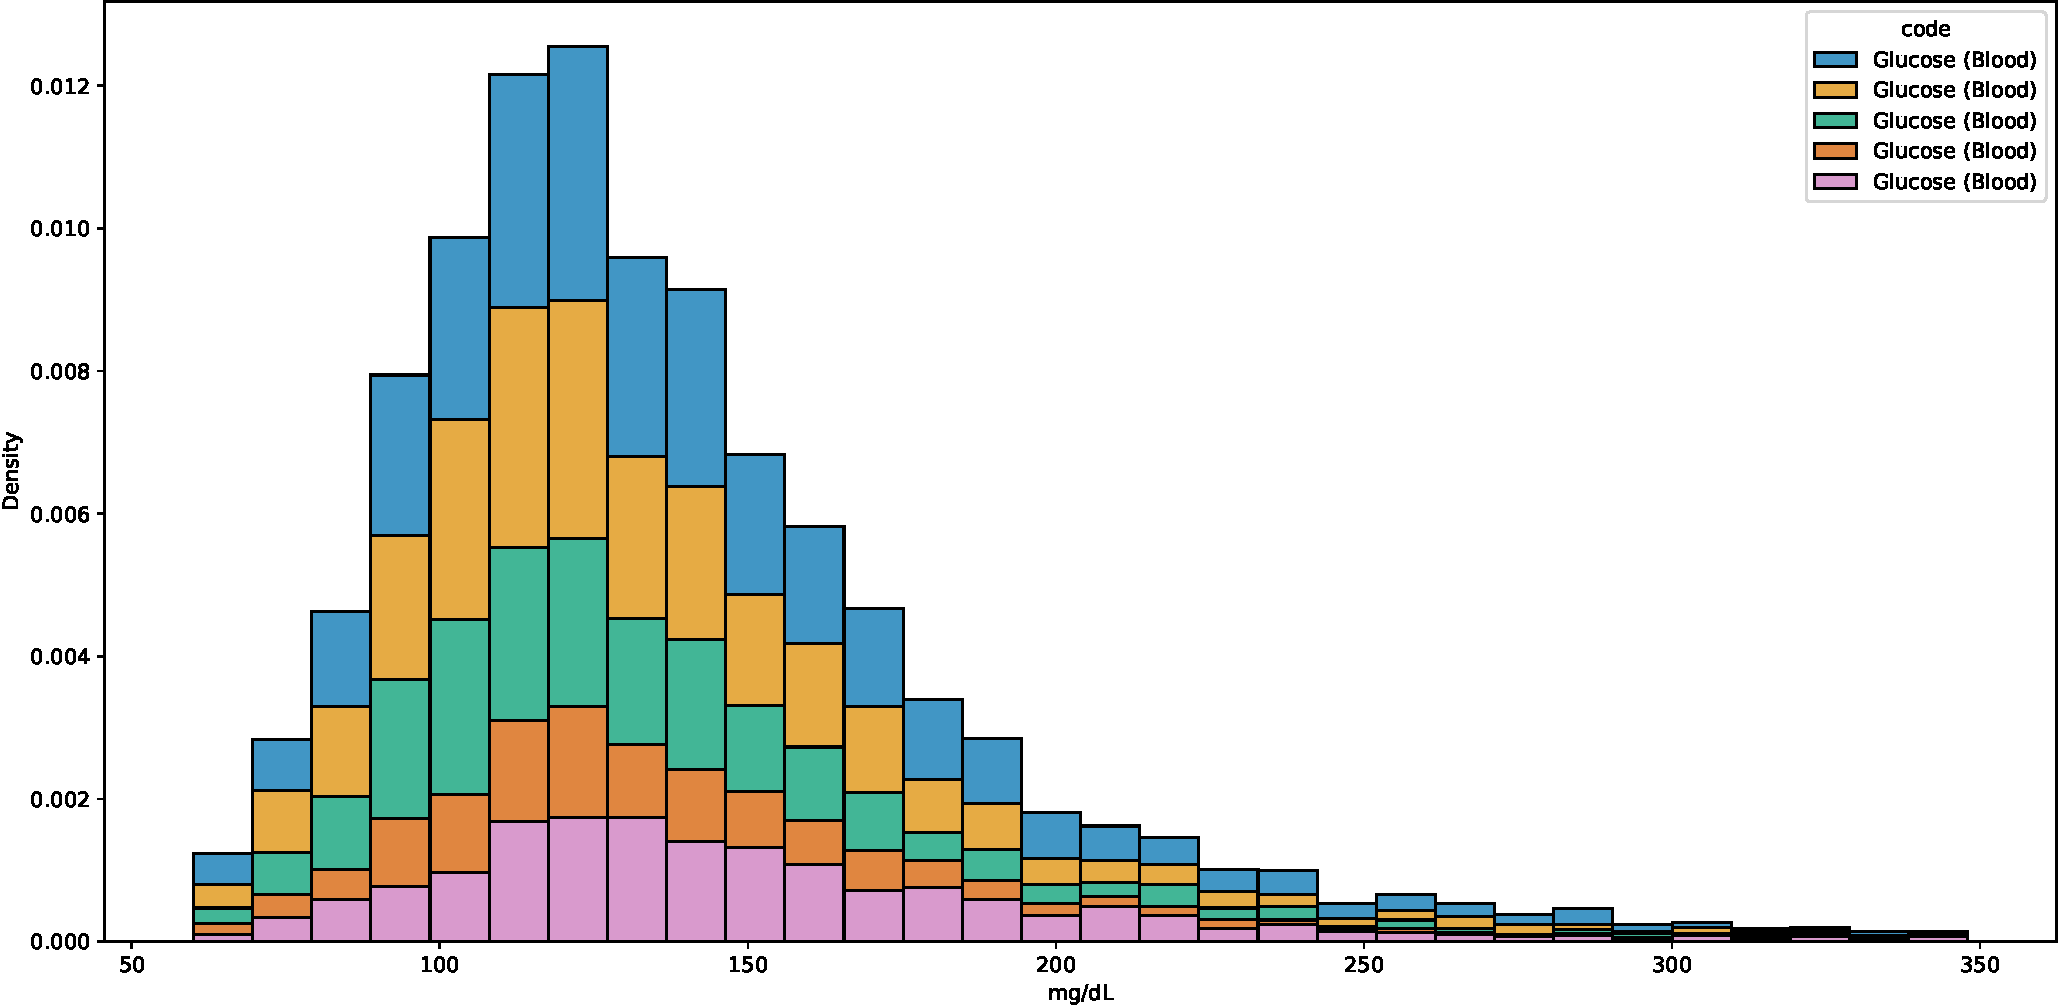
\includegraphics[width=\textwidth]{./figures/hist_Glucose}
    \caption{Distribution of blood glucose values}
    \label{fig:hist_glucose_blood}
\end{figure}

\section{Outlier Processing}
\label{sec:outlier-processing}
Following the methodology described in the original paper, outliers were handled using different strategies based on the type of the event. For each feature, boundaries of valid values were manually defined based on medical expertise and clinical guidelines. Values outside these ranges were identified as outliers and processed accordingly:

\begin{itemize}
    \item \emph{Input and Output Events:} Outliers were replaced with the median value of the respective feature. This approach mitigates the influence of extreme values while preserving the central tendency of the data.
    \item \emph{Chart and Lab Events:} Outliers in these events were removed from the dataset, ensuring analyses were not skewed by erroneous or implausible measurements.
\end{itemize}

Defining valid ranges based on medical knowledge ensured that the outlier detection process was grounded in clinical relevance. For example, physiological measurements that fall outside humanly possible ranges (e.g., a heart rate exceeding \qty{390}{\text{bpm}} or a negative blood pressure) were flagged as outliers.


\section{Value Distributions}

To determine appropriate normalization techniques and understand the characteristics of our data, we analyzed the distributions of the selected features.

Using common normality tests, such as Shapiro-Wilk and Kolmogorov-Smirnov, did not provide satisfactory results due to the large number of observations, which led to extremely small p-values, sometimes beyond \texttt{float32} precision. Therefore, we opted for visual inspection of the distributions and computed skewness ($\gamma$) and excess kurtosis ($\kappa$), as well as the Wasserstein distance ($d_w$) between the Z-transformed observed data and a standard normal distribution. This approach allowed us to identify notable deviations from normality and assess the need for alternative normalization techniques.

Specifically, only \num{25} out of \num{129} features (\qty{19.4}{\percent}) demonstrated relatively low Wasserstein distance from a normal distribution ($d_w < 0.2$), only \num{20} features (\qty{15.5}{\percent}) had low skewness ($|\gamma| < 1$) and only \num{8} (\qty{6.2}{\percent}) had low excess kurtosis (\(|\kappa| < 1 \)). High absolute skewness and high kurtosis indicate asymmetric distributions and heavy tails, which can adversely affect algorithms sensitive to extreme values or non-normality. This motivated us to explore alternative normalization techniques that do not rely on the normality assumption. A detailed statistics for all selected features can be found in \cref{ch:features_statistics}.


\section{Feature Correlations}

Analyzing feature correlations aids in identifying relationships within the dataset, informing feature selection, and guiding model development. Correlation analysis can reveal multicollinearity, where two or more features are highly correlated, which may affect the performance of certain models. It also provides insights into potential dimensionality reduction and reflects underlying biological processes.

Spearman's \( \rho \), a rank correlation coefficient, was used due to the skewed nature of many feature distributions. Spearman's correlation provides a more suitable analysis as it measures the strength and direction of monotonic (but not necessarily linear) relationships between features, making it robust to non-normal distributions and less sensitive to extreme values.

The correlation matrix in \cref{fig:correlation_matrix}, providing an overview of the \num{50} features with highest absolute Spearman's correlations, reveals clusters of highly correlated features. For example, levels of direct, indirect, and total bilirubin are strongly correlated, suggesting they reflect related physiological processes. However, most features exhibit low absolute correlation coefficients, indicating that the selected features provide largely unique information, thus avoiding redundancy. The low absolute rank correlations suggest that capturing relationships between features may require modeling nonlinear and complex interactions, highlighting the potential benefit of advanced modeling techniques.

\begin{figure}
    \centering
    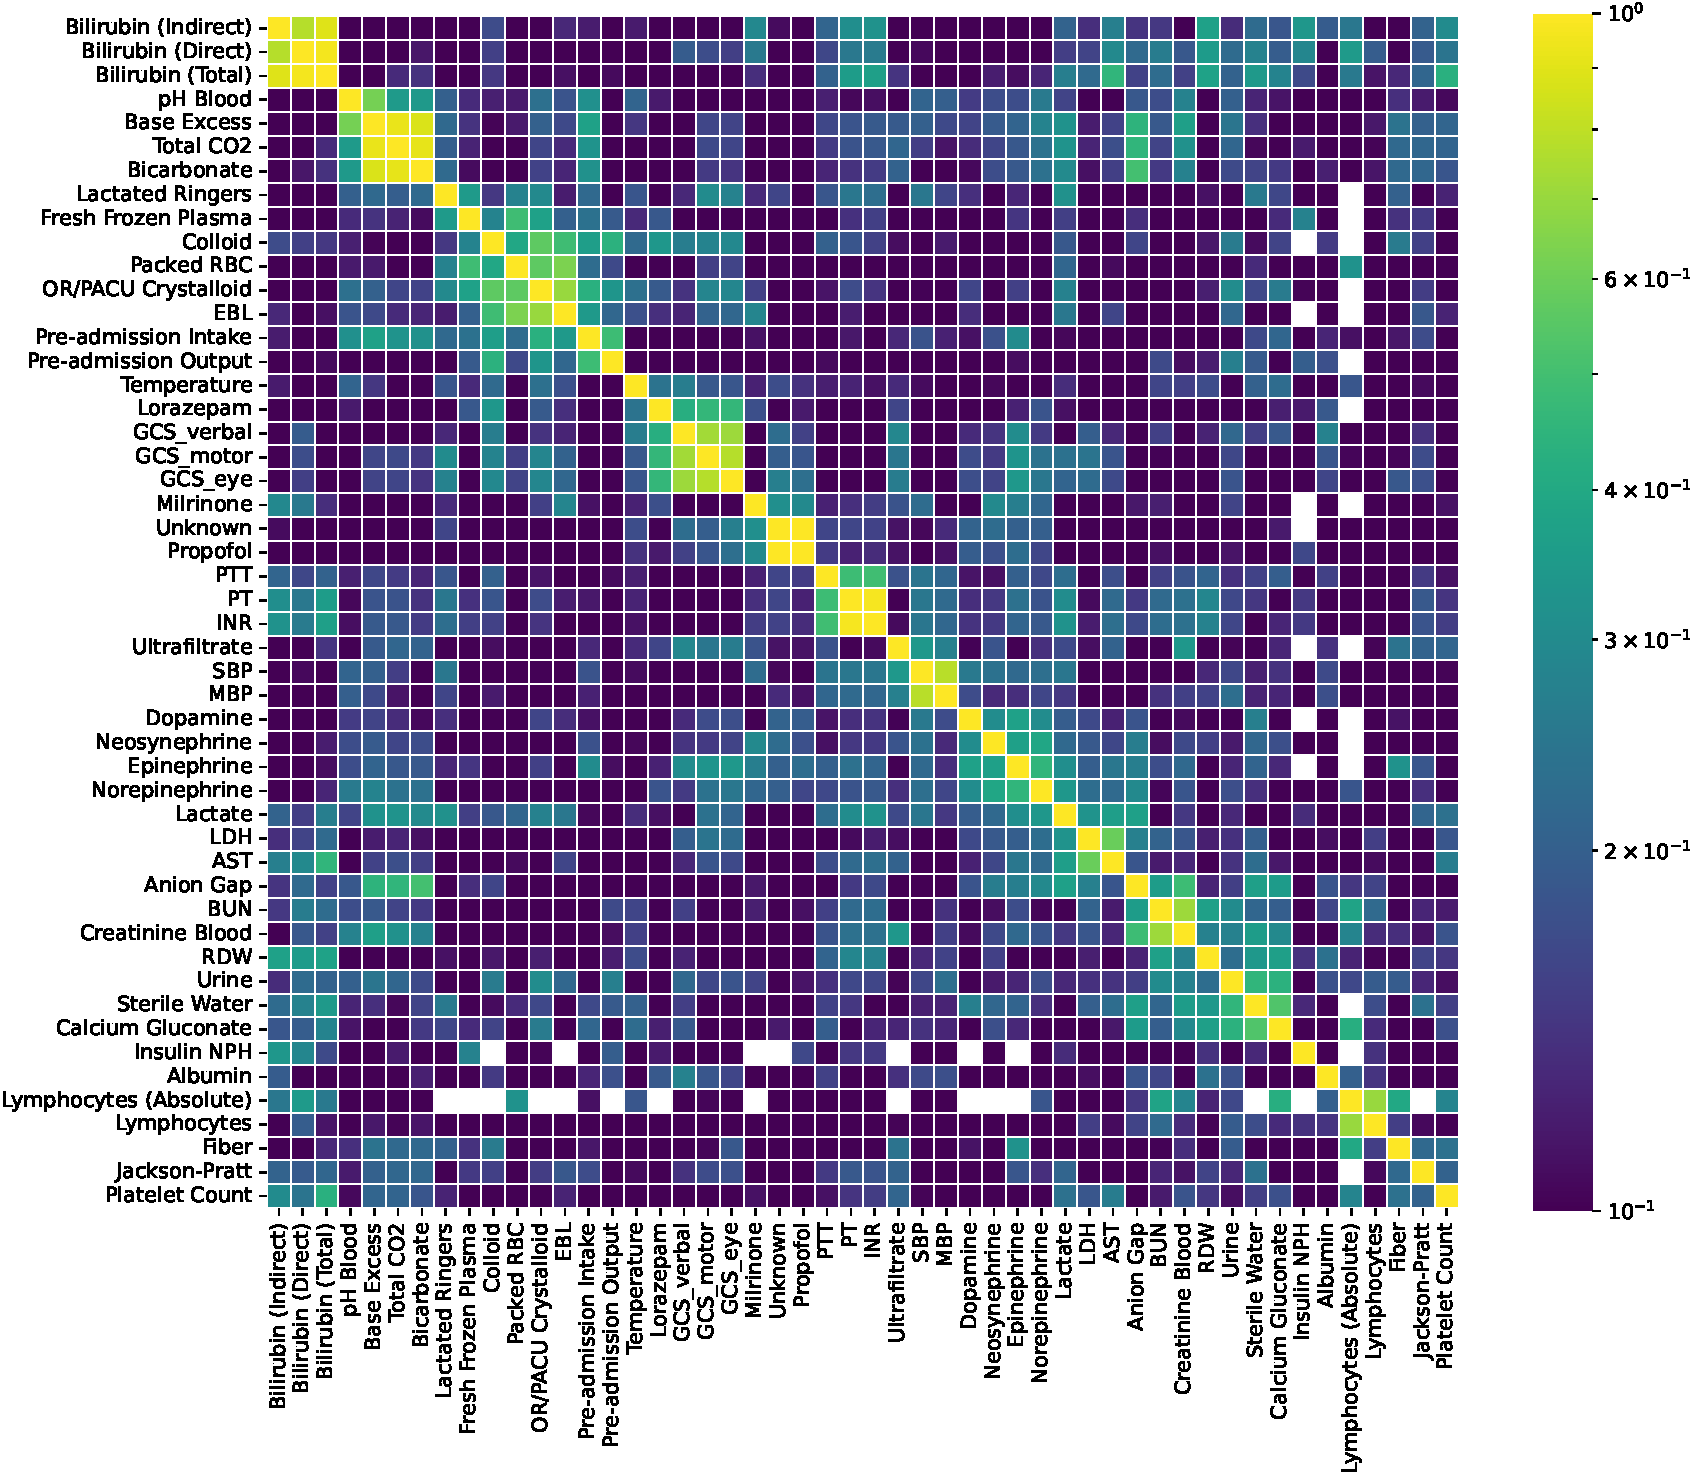
\includegraphics[width=\textwidth]{./figures/correlation_matrix}
    \caption[Spearman $\rho$]{Within-day absolute Spearman correlation of the 50 most correlated features}
    \label{fig:correlation_matrix}
\end{figure}


\section{Patient's Journey Visualizations}

\Cref{fig:journey_292741} illustrates a multivariate clinical time series consisting of \num{\patientJourneyShortLength} observations with irregular time points for a single patient. The Viridis color map indicates the relative value of each measurement compared to other measurements of the same type across the entire dataset, with dark blue representing the lowest values and yellow representing the highest values. To enhance visualization and prevent overlapping, measurements that occur within short time intervals are depicted with smaller circles.

The patient's journey shown in \cref{fig:journey_292741} has fewer observations than the average \gls{icu} stay. On average, an \gls{icu} stay contains \num{1822(4275)} events. For comparison, \cref{ch:patient_journey} presents a visualization of a patient journey with a higher number of measurements.

\begin{figure}
    \centering
    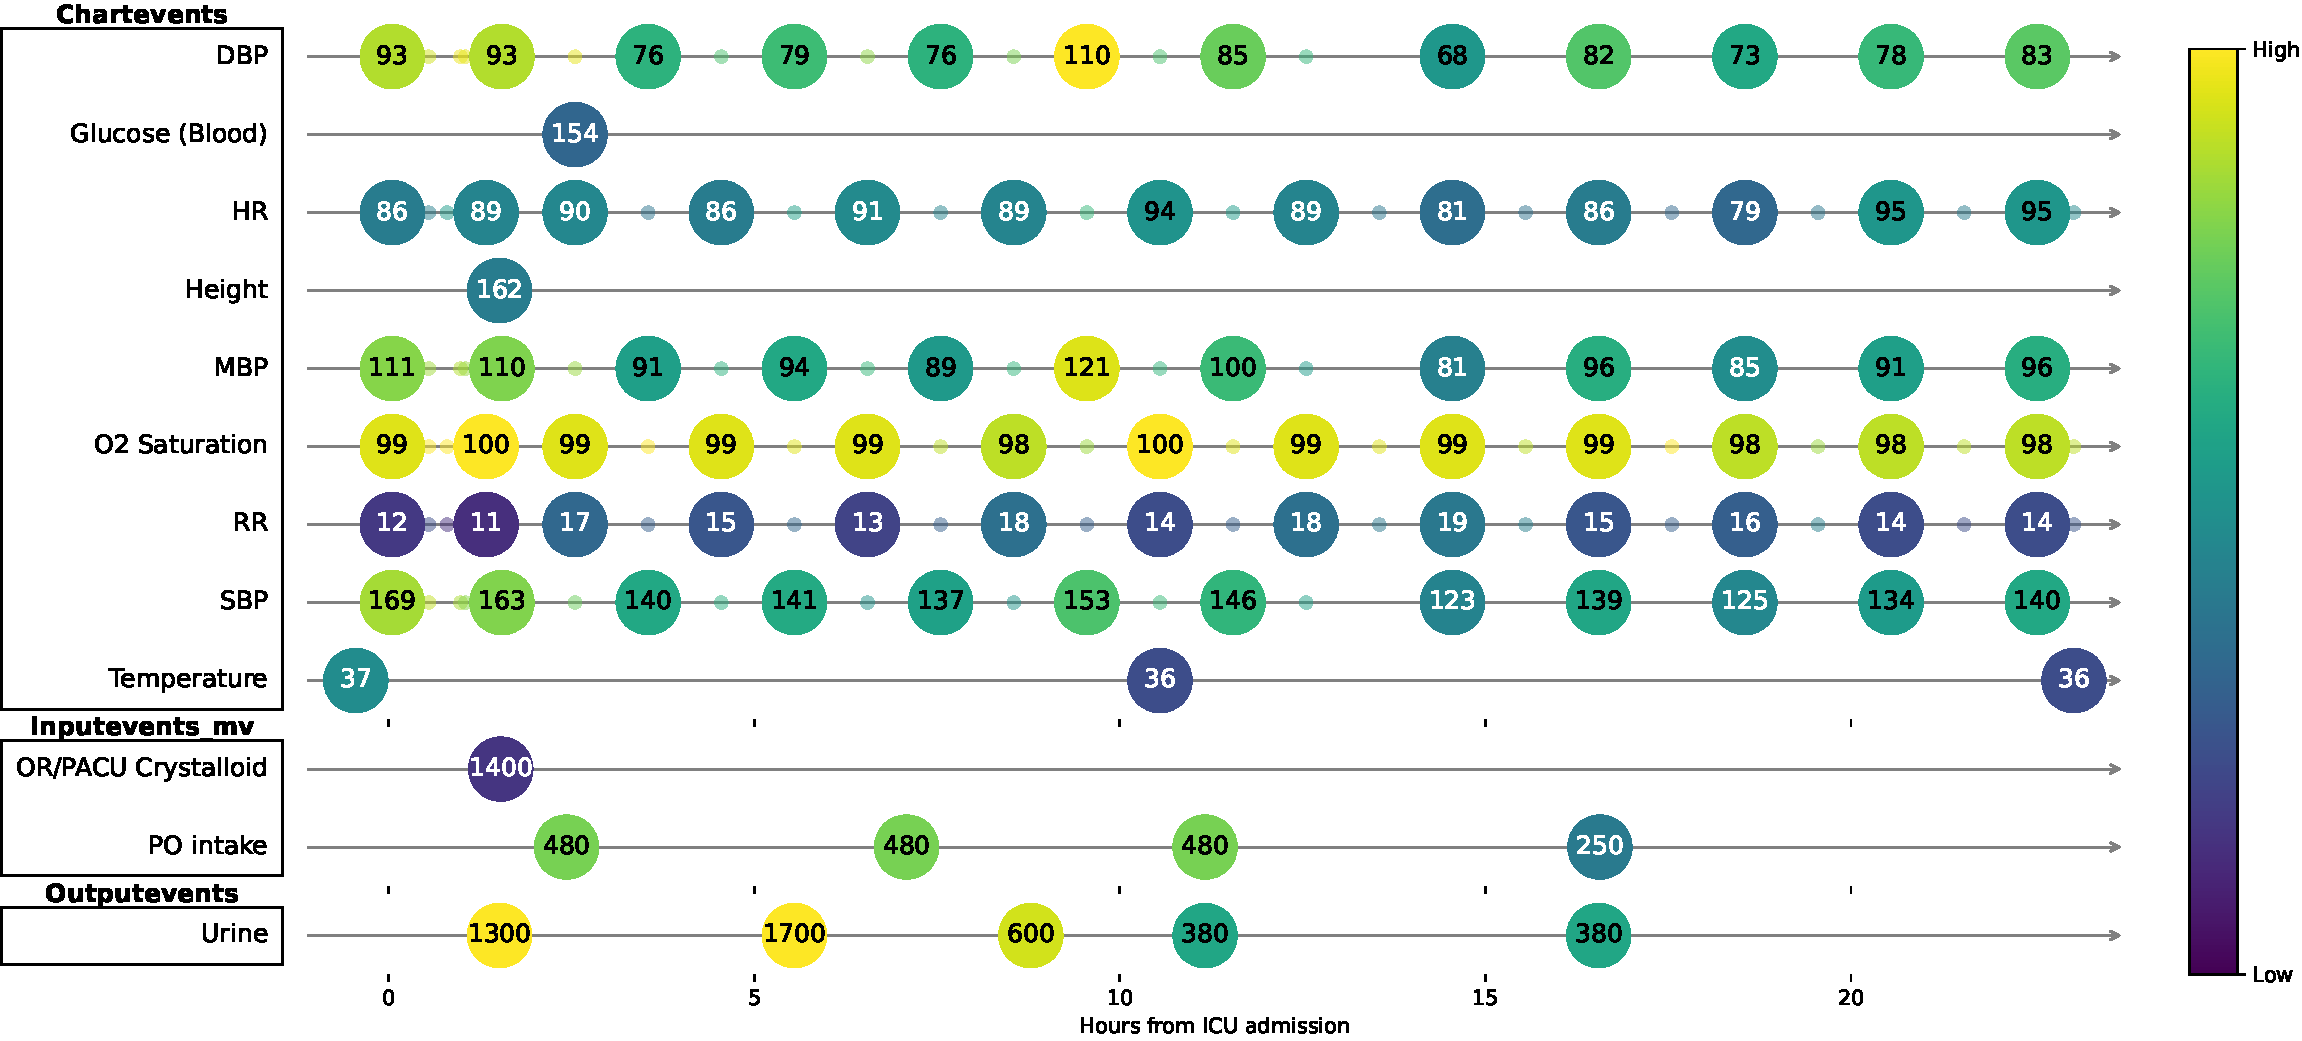
\includegraphics[height=\textheight, width=\textwidth, keepaspectratio]{./figures/journey_292741}
    \caption{Visualization of a multivariate clinical time series with irregular time points and missing values for a single patient}
    \label{fig:journey_292741}
\end{figure}

These visualizations highlight common challenges in clinical health data:

\begin{itemize}
    \item \textbf{Missingness and Sparsity}: Not all features are observed for all patients due to varying clinical needs. As a result, the time-series data are sparse, with some features measured more frequently than others.
    \item \textbf{Irregular Time Intervals}: Clinical measurements are not always taken at regular intervals. The timing of measurements depends on the patient's condition and clinical decisions, leading to sporadic data collection.
\end{itemize}

These challenges complicate data analysis and model development. The handling of missing data and irregular sampling requires advanced methods capable of capturing the temporal dynamics and relationships within the data despite its sparsity and irregularity.


\section{Technical Details of Data Processing}

\subsection{Data Splitting}

To evaluate the generalization capability of the model and prevent data leakage between sets, the dataset was divided into training, validation, and test splits at the patient level \cite{emmert2019evaluation}. The data for each patient are contained entirely within one subset, maintaining the integrity of the evaluation. This patient-level splitting strategy ensures unbiased and reliable performance metrics, providing a solid foundation for model evaluation and comparison.

Following the approach described by \textcite{STraTS2022}, the labeled data were split into a 64:16:20 ratio:

\begin{itemize}
    \item \textbf{Training set} (\qty{64}{\percent}): Used to fit the model's parameters.
    \item \textbf{Validation set} (\qty{16}{\percent}): Used to evaluate model performance during training.
    \item \textbf{Test set} (\qty{20}{\percent}): Reserved for the final evaluation of the model's performance on unseen data.
\end{itemize}

\Cref{tab:split_statistics} presents the distribution of the number of patients in each set.

\begin{table}[h!]
    \centering
    \caption{Statistics of the dataset splits}
    \label{tab:split_statistics}
    \begin{tabular}{lrrr}
\toprule
Split & Number of events & Number of patients & Number of ICU stays \\
\midrule
Unsupervised train & 51,497,384 & 27,289 & 36,849 \\
Supervised train & 49,478,011 & 21,372 & 28,790 \\
Test & 14,886,798 & 6,679 & 8,878 \\
Validation & 11,951,075 & 5,344 & 7,144 \\
\bottomrule
\end{tabular}

\end{table}

\subsection{Data Processing Tools and Technologies}

The data processing pipeline was implemented using Apache Spark \cite{ApacheSpark} and orchestrated with Snakemake \cite{SnakeMake}. This combination allowed for efficient handling of large datasets and reproducible workflow management.

\subsubsection{Apache Spark for Data Processing}

The original data processing pipeline provided by the original paper relied on the Pandas Python library, which required loading the entire dataset into RAM. Due to the large size of the dataset, this approach resulted in excessive memory consumption, causing the Python process to terminate after exhausting \qty{50}{\giga\byte} of RAM (including \qty{20}{\giga\byte} of swap memory).

To address this limitation, the data processing code was rewritten using Apache Spark \cite{ApacheSpark}. Spark's distributed computing capabilities allowed for efficient data processing without the need to load the entire dataset into memory.

Each table of the dataset is provided as a separate CSV file, and collectively they occupy  \qty{39}{\giga\byte} of disk space. The files were converted into a set of Parquet files to enable faster processing and simplify the analysis. The Spark-based pipeline processed the Parquet dataset, utilizing all available \num{16} CPU threads and \qty{16}{\giga\byte} of RAM at peak load, and completed the processing in \qty{5(1)}{\minute}. This represents an order of magnitude speed improvement compared to the original Pandas-based pipeline, which took \qty{53}{\minute} (as was consequently measured after increasing the available RAM to accommodate the process).

Although rewriting the data processing code in Spark provided practical experience and significant performance gains, it required substantial effort and increased the complexity of the codebase. In situations where development time is limited, an alternative approach could be to utilize a cloud virtual machine with more RAM and employ a simpler Pandas-based pipeline if the budget allows.

\subsubsection{Workflow Management with Snakemake}

We used Snakemake to orchestrate all data processing steps. Snakemake is a workflow management system that enables reproducible and scalable execution of complex data workflows. It ensures that each step of the data processing pipeline is executed in the correct order and that dependencies are properly managed, facilitating the reproducibility of the experiments.

\section{Summary}

This chapter has detailed the dataset used in the study, including its structure, the cohort and feature selection process, and the challenges associated with clinical time-series data. The data processing techniques employed, including the use of Apache Spark and Snakemake, were instrumental in efficiently handling the large and complex dataset. Understanding these technical details is crucial for replicating the study and provides a foundation for the modeling approaches discussed in the following chapters.



\chapter{Methodology}
\label{ch:methodology}

This chapter outlines the methodology used in this study, which draws inspiration from the \citetitle{STraTS2022} by \citeauthor{STraTS2022} \cite{STraTS2022}. We aim to extend their approach to address the challenges of mortality prediction using clinical time-series data. The model leverages a transformer-based architecture to generate robust representations of patient data, following a pretraining and fine-tuning strategy.

We begin by presenting the backbone network architecture in \cref{sec:backbone}, which forms the core of our model. The pretraining phase, described in \cref{sec:pretraining}, introduces a self-supervised task where the model learns temporal dynamics through forecasting. The fine-tuning phase in \cref{sec:finetuning} then adapts the pretrained model for mortality prediction.

In subsequent sections, we discuss the training procedure (\cref{sec:training_procedure}), and the implementation details (\cref{sec:implementation_details}). Finally, we compare our approach with several baseline methods in \cref{sec:baselines} and describe the experimental setup in \cref{sec:experiments}.

\paragraph{Notations}

Throughout this chapter, we refer to the ``event'' entities of a \gls{mimiciii} dataset as ``observations'' to maintain consistency with the terminology of the original paper. Furthermore, in this and subsequent chapters we may refer to \textit{fine-tuning stage}, \textit{mortality prediction}, and \textit{time series classification} interchangeably, depending on the context. Similarly, the terms \textit{pretraining stage} and \textit{time series forecasting} can be used interchangeably. Lastly, \cref{tab:model_notations} summarizes the mathematical notations used in this chapter.

\begin{table}[h!]
    \centering
    \caption{Notations used in this section}
    \label{tab:model_notations}
    \begin{tabular}{ll}
\toprule
\textbf{Notation} & \textbf{Definition} \\
\midrule
\(t_i \in \mathbb{R}_{\geq 0}\) & Time of \(i\)th observation \\
\(f_i \in \mathcal{F}\) & Clinical variable of \(i\)th observation \\
\(v_i \in \mathbb{R}\) & Value of \(i\)th observation \\
\(\bar{t}_i, \bar{v}_i\) & Normalized time and value \\
\(\mathbf{T}\) & Multivariate time series \(\{(t_i, f_i, v_i)\}_{i=1}^n\) \\
\(\mathbf{e}_i^f, \mathbf{e}_i^v, \mathbf{e}_i^t \in \mathbb{R}^d\) & Feature, value and time embeddings for \(f_i\) \\
\(\mathbf{e}_i \in \mathbb{R}^d = \mathbf{e}_i^f + \mathbf{e}_i^v + \mathbf{e}_i^t\) & Initial triplet embedding for \(i\)th observation \\
\(\mathbf{E} \in \mathbb{R}^{n \times d}\) & Sequence of triplet embeddings \\
\(\mathbf{C} \in \mathbb{R}^{n \times d}\) & Contextual triplet embeddings \\
\(\alpha_i\) & Attention weight for \(i\)th contextual embedding \\
\(\mathbf{e}^T \in \mathbb{R}^d\) & Time-series embedding \\
\(\mathbf{d} \in \mathbb{R}^D\) & Demographics vector \\
\(\mathbf{e}^d \in \mathbb{R}^d\) & Demographics embedding \\
\(\mathbf{W}_\cdot \in \mathbb{M}\) & Weight matrix \\
\(\mathbf{b}_\cdot \in \mathbb{R}^d\) & Bias vector \\
\(\mathcal{M}, \mathcal{M}_{pt}, \mathcal{M}_{ft}\) & Backbone, pretrained and fine-tuned models \\
\(\mathcal{D}_{\text{split}}, \mathcal{D}'_{\text{split}} \) & Pretraining and fine-tuning datasets for corresponding splits \\
\bottomrule
\end{tabular}

\end{table}

\section{Backbone Network Architecture}
\label{sec:backbone}

In this section, we present the architecture of the backbone model, denoted as \(\mathcal{M}\). The term \textit{backbone} is commonly used in the context of neural networks to refer to the core components of a model that serve as the foundation for subsequent tasks. This backbone model is responsible for generating vector representations (embeddings) from multivariate time-series data, which include both clinical variables and demographic information. This backbone model serves as a \emph{feature extractor}, transforming raw input data into meaningful vector representations.

The architecture described here is \emph{headless}, which means that it excludes the final task-specific layers (or \emph{heads}) typically used for classification or regression. Instead, \(\mathcal{M}\) focuses on producing robust vector embeddings that encapsulate the intricacies of a patient's journey through their \gls{icu} stay. These embeddings can be subsequently fed into various heads, each tailored for specific downstream tasks, such as mortality prediction, length-of-stay estimation, or other clinically relevant outcomes.

The following subsections provide a detailed description of the main components of the backbone model, closely following the structure and notations presented in the original paper.

\subsection{Continuous Value Embedding}
\label{sec:cve}

In their work, \citeauthor{STraTS2022} proposed a \gls{cve} technique using a one-to-many \gls{ffn} with learnable parameters, defined as
\[ \mathbf{e} = \text{FFN}(v) \in \mathbb{R}^d. \]

The \gls{ffn} has one input neuron and \(d\) output neurons, with a single hidden layer containing \(\lfloor \sqrt{d} \rfloor\) neurons and a \(\tanh(\cdot)\) activation function. Formally, it is expressed as:
\[
\text{FFN}(x) = U \tanh(Wx + b),
\]
where \(W \in \mathbb{R}^{\lfloor \sqrt{d} \rfloor \times 1}\), \(b \in \mathbb{R}^{\lfloor \sqrt{d} \rfloor}\), and \(U \in \mathbb{R}^{d \times \lfloor \sqrt{d} \rfloor}\). Unlike commonly used sinusoidal encodings with a fixed set of frequencies, this technique offers more flexibility by allowing end-to-end learning of continuous value embeddings without the need to categorize the input values.

\subsection{Initial Triplet Embedding}

Given an input time series \( \mathbf{T} = \{(t_i, f_i, v_i)\}_{i=1}^n \), where each observation triplet consists of the time \(t_i \in \mathbb{R}_{\geq 0}\), the feature \(f_i \in \mathcal{F}\), and the corresponding value \(v_i \in \mathbb{R}\), the model computes an initial triplet embedding \(\mathbf{e}_i \in \mathbb{R}^d\).

The initial triplet embedding \(\mathbf{e}_i\) is obtained by summing three component embeddings:

\begin{itemize}
    \item \textbf{Feature Embedding} \(\mathbf{e}_i^f \in \mathbb{R}^d\): Maps each feature \(f_i\) to a learnable embedding vector.
    \item \textbf{Value Embedding} \(\mathbf{e}_i^v \in \mathbb{R}^d\): Computed using the \gls{cve} technique applied to the observed value \(v_i\).
    \item \textbf{Time Embedding} \(\mathbf{e}_i^t \in \mathbb{R}^d\): Computed using the \gls{cve} technique applied to the observation time \(t_i\).
\end{itemize}

This step is summarized as:
\[
\mathbf{e}_i = \mathbf{e}_i^f + \mathbf{e}_i^v + \mathbf{e}_i^t.
\]

\subsection{Contextual Triplet Embedding}

The sequence of initial embeddings \(\mathbf{E} = [\mathbf{e}_1, \ldots, \mathbf{e}_n] \in \mathbb{R}^{n \times d}\) is passed through a transformer model composed of \(M\) blocks. Each block includes a \gls{mha} layer with \(h\) attention heads, followed by a \gls{ffn} with a single hidden layer.

The computation for the \(j\)-th attention head in the \gls{mha} layer is given by:
\[
H_j = \text{Softmax}\left(\frac{\mathbf{E} \mathbf{W}^q_j (\mathbf{E} \mathbf{W}^k_j)^\top}{\sqrt{d / h}}\right) \mathbf{E} \mathbf{W}^v_j, \quad \text{for} \quad j = 1, \ldots, h,
\]
where \(\mathbf{W}^q_j, \mathbf{W}^k_j, \mathbf{W}^v_j \in \mathbb{R}^{d \times \lfloor d / h \rfloor}\) are the query, key and value projection matrices for the \(j\)-th head.

The outputs of all attention heads are concatenated and projected as:
\[
\text{MHA}(\mathbf{E}) = \left[ H_1 \, \Vert \, \cdots \, \Vert \, H_h \right] \mathbf{W}_o,
\]
where \(\mathbf{W}_o \in \mathbb{R}^{d \times d}\) is the output projection matrix.

The \gls{ffn} layer is defined as:
\[
\text{FFN}(\mathbf{X}) = \text{GELU}(\mathbf{X} \mathbf{W}_1^f + \mathbf{b}_1^f) \mathbf{W}_2^f + \mathbf{b}_2^f,
\]
where \(\mathbf{W}_1^f \in \mathbb{R}^{d \times 2d}\), \(\mathbf{W}_2^f \in \mathbb{R}^{2d \times d}\), and biases \(\mathbf{b}_1^f \in \mathbb{R}^{2d}\), \(\mathbf{b}_2^f \in \mathbb{R}^d\).

The Gaussian Error Linear Unit (GELU) \cite{gelu} is an activation function defined as:
\[
\text{GELU}(x) = x \cdot \Phi(x),
\]
where \( \Phi(x) \) is the \gls{cdf} of the standard normal distribution.

One key advantage of GELU is that it introduces nonlinearity even in the negative domain, unlike ReLU, which sets negative values to zero. Furthermore, GELU is differentiable across the entire input domain, whereas ReLU is not differentiable at zero. This smoothness improves the model optimization by gradient descent, providing more stability during training.

The output of the transformer, denoted as \(\mathbf{C} = [\mathbf{c}_1, \dots, \mathbf{c}_n]^\top \in \mathbb{R}^{n \times d}\), captures the contextual dependencies among the triplets. It is computed using residual connections in a post-norm architecture as follows:

\[
\mathbf{A} = \text{LayerNorm}_1\left(\text{MHA}(\mathbf{E}) + \mathbf{E}\right),
\]
\[
\mathbf{C} = \text{LayerNorm}_2\left(\text{FFN}(\mathbf{A}) + \mathbf{A}\right)
\]

where \(\text{LayerNorm}_1\) and \(\text{LayerNorm}_2\) are layer normalization functions applied to the output of the \gls{mha} and \gls{ffn} layers, respectively.

\subsection{Fusion Self-Attention}
\label{sec:fusion_self_attention}

To integrate the contextual embeddings into a unified time-series representation, a self-attention mechanism inspired by those used in natural language processing is employed. This mechanism allows the model to weigh the importance of each contextual embedding \(\mathbf{c}_i\) when forming the overall time-series embedding \(\mathbf{e}^T\).

First, an attention score \(a_i\) is computed for each contextual embedding:

\[
a_i = \mathbf{u}_a^\top \tanh(\mathbf{W}_a \mathbf{c}_i + \mathbf{b}_a),
\]

where $\mathbf{W}_a\in \mathbb{R}^{d \times d}, \mathbf{b}_a\in\mathbb{R}^{d}, \mathbf{u_a}\in\mathbb{R}^{d}$ are the weights of this fusion attention network.

Next, the attention scores are converted into normalized weights using the softmax function:

\[
\alpha_i = \frac{\exp(a_i)}{\sum_{j=1}^{n} \exp(a_j)}.
\]

The attention weights \(\alpha_i\) reflect the relative importance of each time step in the sequence.

Finally, the time-series embedding is computed as a weighted sum of the contextual embeddings:

\[
\mathbf{e}^T = \sum_{i=1}^{n} \alpha_i \mathbf{c}_i.
\]

This process aggregates the entire sequence into a single vector, emphasizing the most relevant observations based on the learned attention weights.

\subsection{Demographics Embedding}
\label{sec:demographics_embedding}

Demographic information \(\mathbf{d} \in \mathbb{R}^D\) is incorporated into the model through a separate embedding process. The demographics embedding \(\mathbf{e}^d \in \mathbb{R}^d\) is computed by passing \(\mathbf{d}\) through a \gls{ffn}:
\[
\mathbf{e}^d = \mathbf{W}_1^d \tanh\left( \mathbf{W}_2^d \mathbf{d} + \mathbf{b}_2^d \right) + \mathbf{b}_1^d,
\]
where \(\mathbf{W}_1^d \in \mathbb{R}^{d \times 2d}\), \(\mathbf{W}_2^d \in \mathbb{R}^{2d \times D}\), \(\mathbf{b}_1^d \in \mathbb{R}^{d}\), and \(\mathbf{b}_2^d \in \mathbb{R}^{2d}\) are learnable parameters. This process resembles the \gls{cve} technique, with the primary difference being the size of the hidden layer and number of input neurons.


\subsection{Integrated Vector Representation}

The backbone network generates embeddings for both clinical time-series data and demographic information. The final output of the backbone network is a concatenated vector representation that integrates these embeddings.

Formally, the complete embedding produced by the model is expressed as:
\[
\mathcal{M}(\mathbf{T}, \mathbf{d}) = \mathbf{e}^d \Vert \mathbf{e}^T,
\]
where \( \mathbf{e}^d \) represents the demographics embedding and \( \mathbf{e}^T \) denotes the time-series embedding. This integrated representation \( \mathcal{M} \) serves as the input for subsequent model components, which are tailored to different downstream tasks such as forecasting or classification.


By integrating the embeddings of clinical time-series data and demographic information, the backbone network produces a vector representation that captures both temporal dynamics and patient characteristics.

\section{Training Procedure}
\label{sec:training_procedure}

In this section, we outline the training procedure employed to develop our model, including data preprocessing, optimization configurations, and model selection strategies.

\subsection{Data Preprocessing}

The training process begins with data loading and preprocessing. We apply Z-score normalization to standardize the values in observation triplets and the age, ensuring that each has a mean of zero and a standard deviation of one. This standardization is beneficial when dealing with features of varying scales, as it ensures that each feature have similar scale and magnitude and thus contributes equally to the model's learning process.

The standardized value \( \bar{v} \) for a feature \( f \) is calculated as:

\[
\bar{v} = \frac{v - \mu_f}{\sigma_f},
\]

where \( v \) is the original value, \( \mu_f \) is the mean, and \( \sigma_f \) is the standard deviation of feature \( f \) computed from the training data.

\subsubsection*{Variable Dropout}
\label{sec:variable_dropout}

Variable dropout is a form of data augmentation that involves randomly dropping out a subset of features (variables) from the input sequence during training. This technique helps prevent overfitting by encouraging the model to learn robust representations that do not rely on any single feature \cite{DropoutSimpleWay2014}. By simulating missing features during prediction, this technique improves the model's ability to handle incomplete data in real-world applications.

Specifically, we exclude a random subset of features from the entire input sequence with a probability \(p = 0.2\), meaning that for each feature \(f_i\), we decide whether to drop it across all time steps. This process is formally expressed as:
\begin{equation}
    \label{eq:variable_dropout}
    \mathbf{T}' = \left\{ (t_i, f_i, v_i) \in \mathbf{T} \,\big|\, r_{f_i} = 1 \right\}, \quad \text{where } r_{f_j} \sim \text{Bernoulli}(1 - p), j = 1, \dots, |\mathcal{F}|.
\end{equation}

Here, \(\mathbf{T}\) represents the original set of events, and \(r_{f_i}\) is a binary variable indicating whether feature \(f_i\) is retained (\(r_{f_i} = 1\)) or dropped (\(r_{f_i} = 0\)). The modified time series  \(\mathbf{T}'\) thus consists only of a subset of retained feature observations.

\subsection{Optimization Configuration}

The optimization process involves configuring the training parameters to efficiently minimize the loss function. Key components include the choice of optimizer, batch size, learning rate, and regularization techniques.

\subsubsection{AdamW Optimizer}

We utilize the AdamW optimizer \cite{DecoupledWeightDecay2019}, an extension of the Adam optimizer that decouples weight decay from the gradient update rule. Weight decay, a form of L2 regularization, helps prevent overfitting by penalizing large weight values. In AdamW, weight decay is applied directly to the model weights, which typically results in better generalization performance.

The update rule for AdamW is:

\[
\theta_{t+1} = \theta_t - \eta \left( \frac{m_t}{\sqrt{v_t} + \epsilon} + \lambda \theta_t \right),
\]

where \(\theta_t\) represents the model parameters at time \(t\), \(\eta\) is the learning rate, \(m_t\) and \(v_t\) are the first and second moment estimates of the gradients, \(\epsilon\) is a small constant to prevent division by zero, and \(\lambda\) is the weight decay coefficient.

In contrast to the original study, we disabled weight decay for the norm and bias parameters. This is a common practice in deep learning because applying weight decay to these parameters can be counterproductive\cite{BagTricksImage2018}.

\subsubsection{Batch Size and Learning Rate}

We use a batch size of \num{16} for both pretraining and fine-tuning stages, balancing computational efficiency and gradient estimation stability.

The learning rate is set to \(1 \times 10^{-4}\) during pretraining and reduced to \(1 \times 10^{-5}\) during fine-tuning. A smaller learning rate in the fine-tuning phase allows for more precise updates and helps prevent divergence from the pretrained parameters.

\subsection{Model Selection}

Model selection involves evaluating and choosing the model configuration that best generalizes to unseen data. We employ validation and early stopping strategies to prevent overfitting and select optimal model parameters.

We use a validation set, distinct from the training data, to monitor the model's performance during training. After each epoch, the model is evaluated on the validation set using the defined evaluation metrics. This process provides insights into the model's generalization ability and helps detect overfitting.

Early stopping is implemented to halt training when the model's performance on the validation set ceases to improve. Specifically, if no improvement is observed in the validation loss after 10 epochs, known as the \emph{patience} parameter, training is stopped and the model with the best validation performance is restored.

\section{Pretraining Phase}
\label{sec:pretraining}

The pretraining phase aims to improve the model's ability to learn general temporal dynamics in clinical time-series data without relying on limited labeled samples. This phase enables the model to develop robust embeddings from unlabeled data, which are later fine-tuned for specific tasks, such as mortality prediction. In the referenced study, pretraining on a self-supervised forecasting task was shown to improve the final model's performance (\gls{auroc} \( +0.01 \), \gls{aucpr} \( +0.03 \). \gls{minrp} \( +0.02 \)).
\citeauthor{STraTS2022} concluded that the model pretraining ``enables learning generalized vector representations in the presence of limited labeled data and alleviates sensitivity to noise''.

In this section, we describe the data \( \mathcal{D} \), model \( \mathcal{M}_{pt} \) and the loss function used for optimizing the model during this phase.


\subsection{Unlabeled Data}

The model utilizes a dataset \( \mathcal{D} = \{(\mathbf{d}_i, \mathbf{T}_i, \mathbf{m}_i, \mathbf{z}_i)\}_{i=1}^{N} \), where \( N \) is the number of samples (i.e., \gls{icu} stays). The input time series \( \mathbf{T}_i = \{(v_j, t_j, f_j)\}_{j=1}^{n} \) is represented by three vectors of equal length: \( \mathbf{v} \) for feature values, \( \mathbf{t} \) for corresponding timestamps, and \( \mathbf{f} \) for feature identifiers.

The input time series consists of observation triplets within a random \qtyrange{12}{24}{\hour}  window, defined by the interval \([t_0, t_1]\), where \( t_1 \in [\qty{12}{\hour}; t_n ) \) is chosen randomly such that window is at least \qty{12}{\hour} and at least a single observation falls within prediction window. The start time is then \( t_0 = \max(t_1 - \qty{24}{\hour}, \qty{0}{\hour}) \).

To facilitate model training, the time values are normalized to the interval \([-1, 1]\):
\begin{equation}
    \label{eq:normalize_time}
    \bar{t}_j = \frac{t_j - t_0}{\qty{12}{\hour}} - 1 \in [-1, 1] \quad j = 1, \dots, n,
\end{equation}
where \( n \) is the number of observations in the time series.

Thus, the selected \qtyrange{12}{24}{\hour} time series is defined as:
\begin{equation}
    \label{eq:input_24_window}
    \mathbf{T}_{\qty{24}{\hour}} = \left\{ \left( \bar{t}_j, \, f_j, \, \bar{v}_j \right) \ \middle|\ t_0 \leq t_j \leq t_1 \right\}_{j = 1}^{n}.
\end{equation}

The selected time series then undergoes random variable dropout, as described in \cref{sec:variable_dropout}, to simulate missing features in the input sequence. To limit the memory requirements of the model, we the number of observations in a time series is limited to a maximum of \num{880}. If the number of observations within the time window exceeds this limit, random observations are removed to reduce the sequence length.

The model's predictions are defined as a vector of average observed values within a \qty{2}{\hour} prediction window, computed as follows:
\begin{equation}
    \label{eq:forecast_target}
    \mathbf{z}_i = \frac{1}{\| \mathbf{v}_{i,f} \|_0 } \sum^{t_2}_{t=t_1} v_{i,t,f} \in \mathbb{R}^{|\mathcal{F}|},
\end{equation}
where \( t_2 = t_1 + \qty{2}{\hour} \) is the end of the prediction window, \( v_{i,t,f} \) is the value of feature \( f \) at time \( t \), and \( \| \mathbf{v}_{i,f} \|_0 \) is the number of times feature \( f \) was observed within the prediction window.

The corresponding forecast mask \( \mathbf{m}_i \in \{0, 1\}^{|\mathcal{F}|} \) indicates which features were observed at least once during the prediction window. This mask is used to exclude unobserved features from the training process by masking them out during loss computation.

This approach allows the model to leverage both labeled and unlabeled time-series data by selecting different observation windows, thereby increasing the dataset's diversity and size. The upper part of \cref{fig:model_input} illustrates the construction of inputs for the forecasting task. The input structure consists of the three vectors, along with the demographic values \( \mathbf{d} \). The forecast mask \( \mathbf{m} \) and target values \( \mathbf{z} \) are used to compute the loss during training.


\begin{figure}
    \centering
    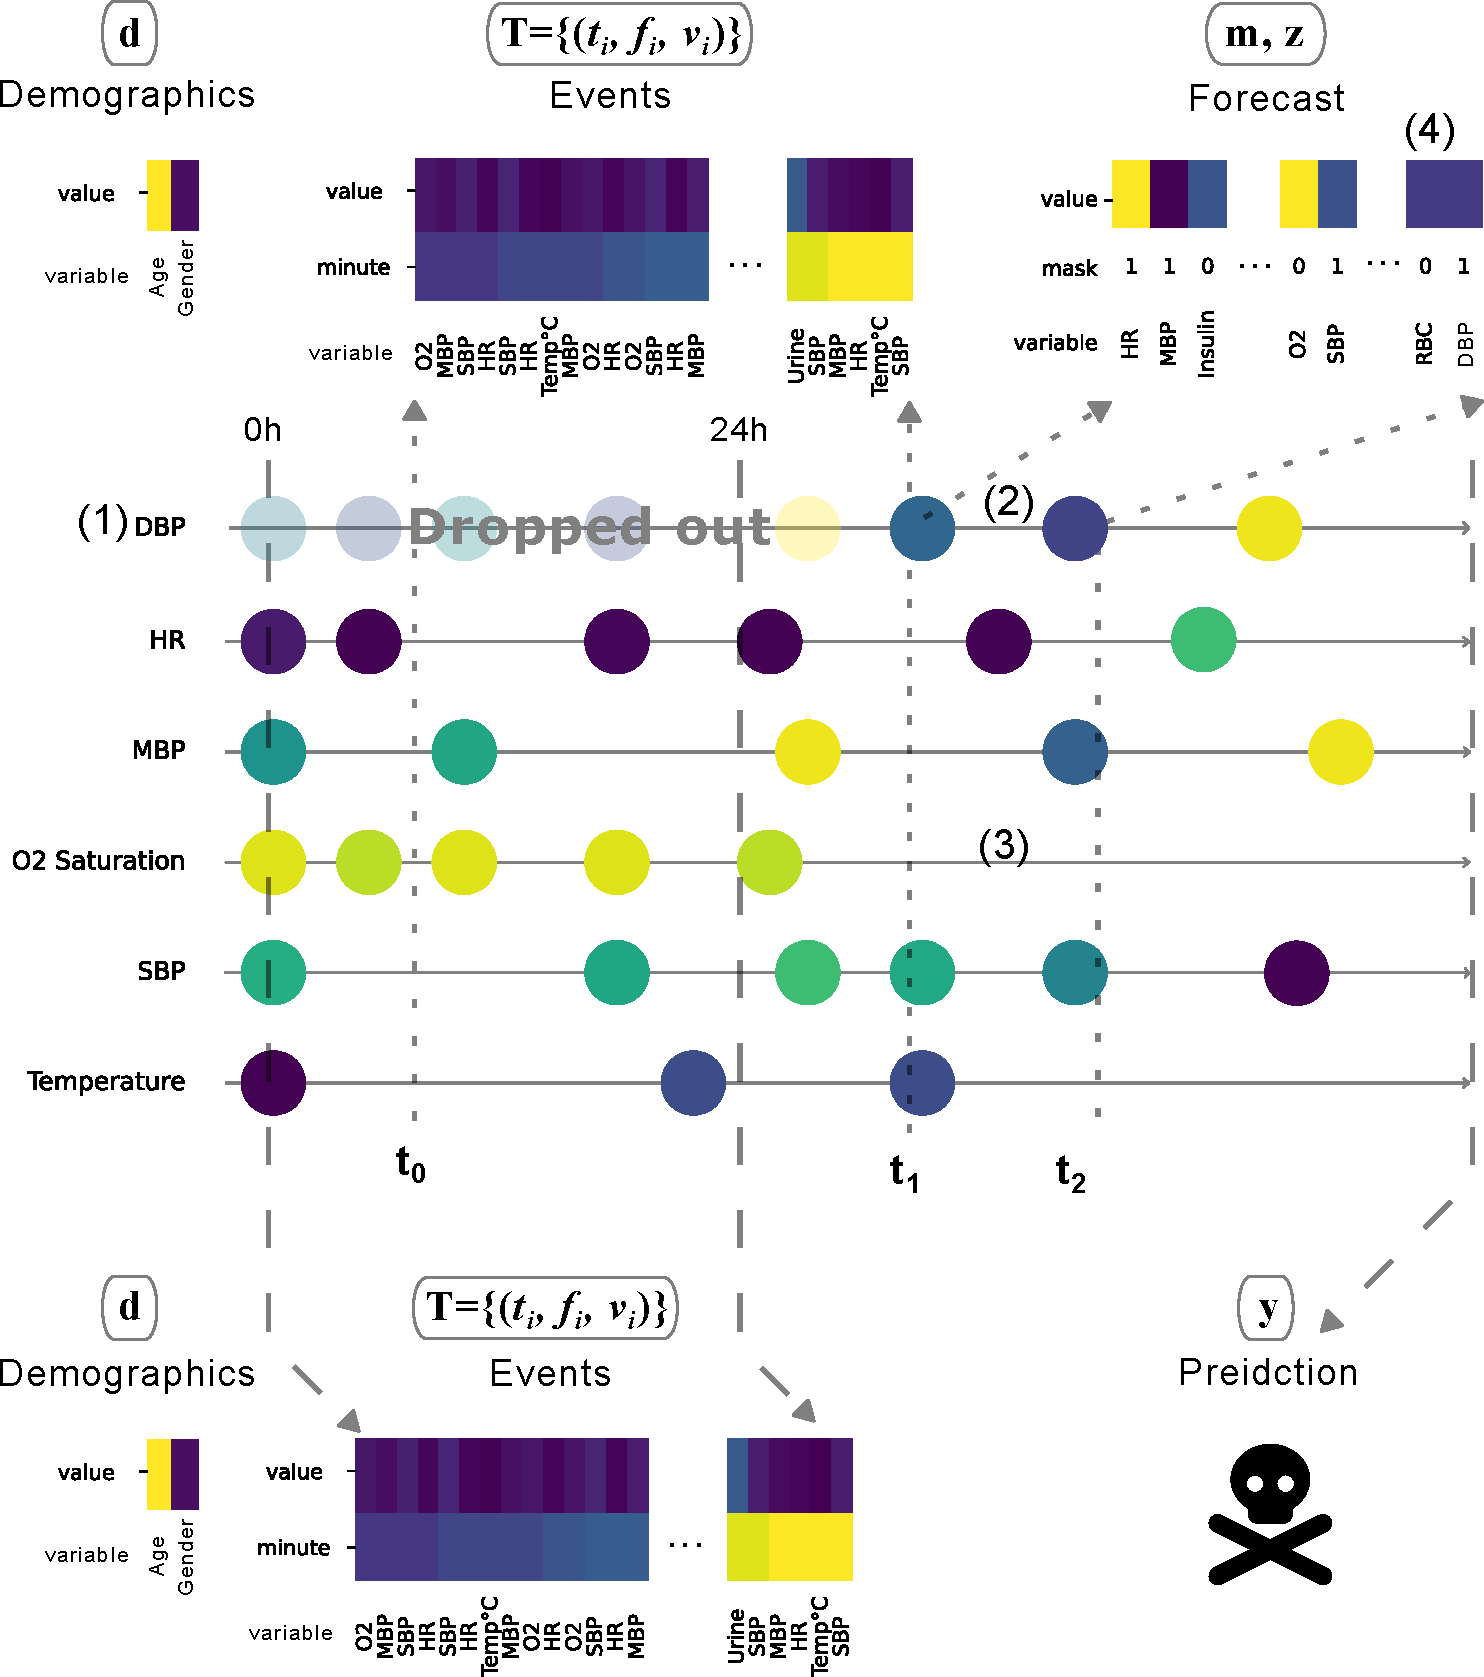
\includegraphics[width=\textwidth]{./figures/model_input}
    \caption{Visualization of the input structure for the forecasting and mortality prediction tasks.
    The DBP time series was excluded from input by a random variable dropout (1). Meanwhile  the mask for DBP has value 1 because it was observed in the data and participates in the forecast loss (2). The forecast mask for O2 Satuaration is 0 because it was not observed in the forecast window (3). RBC has mask 0 because it is not present in the observed data (4).}
    \label{fig:model_input}
\end{figure}

\subsection{Pretrained Model}

During the pretraining phase, the backbone model described in \cref{sec:backbone} is extended by adding a single-layer \gls{ffn} as a forecasting head \( \mathcal{M}_{pt}(\mathbf{d}_i, \mathbf{T}_i) = \mathbf{W}_f \cdot \mathcal{M} + \mathbf{b}_f = \hat{\mathbf{z}} \in \mathbb{R}^{|\mathcal{F}|} \) with parameters \( \mathbf{W}_f \in \mathbb{R}^{d \times \mathcal{F}|} \) and \( \mathbf{b}_f \in \mathbb{R}^{|\mathcal{F}|} \) that maps the integrated vector representation produced by a backbone network to a vector of feature value predictions. The detailed algorithm of pretraining phase is provided in \cref{algorithm:pretrain}.

This configuration is designed to perform a regression task, specifically forecasting future values of the time-series data. The goal of this phase is to pretrain the model, allowing it to learn temporal dynamics and generate robust embeddings that can be used for various downstream tasks.

% TODO: picture of heads

\subsection{Masked Mean Squared Error Loss}

The model's output vector covers all possible features. However, not all features may be observed in the given data. To avoid computing errors for unobserved features, we apply a masked \gls{mse} loss function, evaluating the prediction error only for the features observed within prediction timeframe. It calculates the average of the squared differences between the predicted values \(\hat{z}_i\) and the true values \(z_i\), for the observed features.

\begin{equation}
    \label{eq:mmse}
    \mathcal{L}_{\text{mMSE}}( \mathbf{z}, \hat{\mathbf{z}}, \mathbf{m}) = \frac{\mathbf{m}^\top \cdot (\hat{\mathbf{z}} - \mathbf{z})^{\odot 2}}{\|\mathbf{m}\|_1}  ,
\end{equation}

where

\begin{itemize}
\item \( \mathbf{m} \in {0, 1}^|\mathcal{F}|\) is the mask vector indicating which features were observed,
\item \( (\cdot)^{\odot 2} \) denotes element-wise squaring,
\item \( \|\mathbf{m}\|_1 \) is the sum of the elements of the mask vector (i.e., the number of non-masked values).
\end{itemize}

This formulation ensures that only predictions for observed features contribute to the loss calculation.


\begin{algorithm}[h]
\setstretch{1.35}
\caption{Model Pretraining}
\label{algorithm:pretrain}
\KwData{\( \mathcal{D}_{train},\mathcal{D}_{val},\mathcal{D}_{test} = \{(\mathbf{d}_i, \mathbf{v}_i, \mathbf{t}_i, \mathbf{f}_i)\}_{i=1}^{N} \) }
\KwResult{Pretrained model \(\mathcal{M}_{pt}\) with minimal validation loss \( \mathcal{L}^{val}_{mMSE} \)}

\textbf{Data Preparation:} \\
\nl Standardize feature values: \(\bar{v}_f = \frac{v_f - \mu_f}{\sigma_f}\) \;

\textbf{Training:} \\
\ForEach{epoch until validation loss \(\mathcal{L}^{val}_{mMSE} \) stops decreasing} {
    \nl Initialize accumulated loss \(\mathcal{L}_{acc} = 0\) \;
    \ForEach{\(i \in [1, N] \)} {
        \nl Sample input data: \( \mathbf{T}_{\qty{24}{\hour}} \) \tcp*[l]{see \cref{eq:input_24_window}} \label{alg:pretrain_epoch_start}
        \nl Apply variable dropout: \( \mathbf{T}'_{\qty{24}{\hour}} \) \tcp*[l]{see \cref{eq:variable_dropout}}
        \nl Compute target vector: \( \mathbf{z} \in \mathbb{R}^{|\mathcal{F}|} \) \tcp*[l]{see \cref{eq:forecast_target}}
        \nl Compute forecast mask: \(\mathbf{m} \in \{0, 1\}^{|\mathcal{F}|}\) \;
        \nl Forecast values: \(\hat{\mathbf{z}} = \mathcal{M}_{pt}(\mathbf{d}_i,\mathbf{T}'_{\qty{24}{\hour}}) \) \;
        \nl Accumulate loss: \(\mathcal{L}_{acc} \mathrel{+} = \mathcal{L}^{train}_{mMSE} (\mathbf{z}_i, \hat{\mathbf{z}}_i, \mathbf{m}) \) \tcp*[l]{see \cref{eq:mmse}} \label{alg:pretrain_compute_loss}
        \If{\(i \mod \text{batch size} = 0\)} {
            \nl Backpropagate and update model weights \;
            \nl Reset accumulated loss \(\mathcal{L}_{acc} = 0\) \;
        }
    }
    \nl Repeat \crefrange{alg:pretrain_epoch_start}{alg:pretrain_compute_loss} for \(\mathcal{D}_{val}\) and compute validation loss \(\mathcal{L}^{val}_{mMSE} \) \;
}
\textbf{Evaluation:} \\
\nl Repeat \crefrange{alg:pretrain_epoch_start}{alg:pretrain_compute_loss} for \(\mathcal{D}_{test}\) and compute test loss \(\mathcal{L}^{test}_{mMSE} \) \;
\end{algorithm}



\subsection{Summary of Pretraining Phase}

\begin{itemize}
    \item \emph{Task}: Time series forecasting.
    \item \emph{Data}: Demographics + random \qty{24}{\hour} time-series window without labels.
    \item \emph{Model}: Backbone model appended by a single-layer \gls{ffn} (forecast head).
    \item \emph{Loss}: masked Mean Squared Error loss.
    \item \emph{Learning type}: Self Supervised.
    \item \emph{Purpose}: Pretraining the model to learn temporal dynamics and generate useful embeddings for downstream tasks.
\end{itemize}

%%%%%%%%%%%%%%%%%%%%%%%%%%%%%%%%%%%%%%%%%%%%%%


\section{Fine-tuning Phase}
\label{sec:finetuning}

The fine-tuning phase involves adapting the pretrained model to specific downstream tasks, particularly binary classification tasks such as mortality prediction. In the mortality prediction, the model \( \mathcal{M}_{ft} \) must determine whether a patient is likely to survive based on data available within the first \qty{24}{\hour} of an \gls{icu} stay. Building upon the temporal dynamics learned during pretraining, the model is fine-tuned to optimize its performance for this specific supervised learning objective.

\subsection{Labeled Data}

Consider a labeled dataset \( \mathcal{D}' = \{(\mathbf{d}_i, \mathbf{T}_i, y_i)\}_{i=1}^{N'} \), where \(N'\) represents the number of labeled samples. Here, \( y_i \in \{0, 1\} \) is a binary label that indicates the patient's outcome, e.i. the mortality during the hospital stay. The number of labeled samples \( N' \) may be smaller than \( N \) due to the lack of additional labeled data. The model must accurately determine whether a patient is likely to survive based on the input data from the first \qty{24}{\hour} of the \gls{icu} stay so only a fraction of entire time series is selected, corresponding to using \( t_0 = 0 \) and \( t_1 = \qty{24}{\hour}\) in \cref{eq:normalize_time}. The time series is then defined as

\begin{equation}
    \label{eq:first_24_window}
    \mathbf{T}_{\qty{24}{\hour}} = \left\{ \left( \bar{t}_j, \, f_j, \, \bar{v}_j \right) \ \middle|\ t_j \leq \qty{24}{\hour} \right\}_{j = 1}^{n}.
\end{equation}

The bottom part of \cref{fig:model_input} illustrates the construction of inputs for the mortality prediction task. Similarly to the previous phase, the input structure consists of three vectors: the feature values \( \mathbf{v} \), the corresponding timestamps \( \mathbf{t} \), and the feature identifiers \( \mathbf{f} \), along with the demographics values \( \mathbf{d} \), but in contrast with the forecasting task the selected time series is always the first \qty{24}{\hour} of the \gls{icu} stay. Additionally, the binary label \( y \) is used to compute the loss during training.

\subsection{Fine-tuned Model}

During this phase, the pretrained forecasting model \(\mathcal{M}_{pt} \), as described in \cref{sec:pretraining}, is extended by adding a single neuron with a sigmoid activation function, thus acting as a classification head:
\[
    \mathcal{M}_{ft}(\mathbf{d}_i, \mathbf{T}_i) = \text{sigmoid}(\mathbf{W}_c \cdot \mathcal{M}_{pt}(\mathbf{d}_i, \mathbf{T}_i) + \mathbf{b}_c) = \hat{y}_i \in [0, 1]
\]

where \(\mathbf{W}_c \in \mathbb{R}^{|\mathcal{F}| \times 1}\) and \(\mathbf{b}_c \in \mathbb{R}\) are the layer weights and bias, respectively. The output \(\hat{y}_i\) represents the predicted probability of mortality for a given patient.

\subsection{Weighted Binary Cross-Entropy Loss}

\Gls{bce} is a loss function commonly used in binary classification problems where the target variable has two possible outcomes, \num{0} and \num{1}. It measures the performance of a classification model whose output is a probability value between \num{0} and \num{1}, indicating the likelihood of the positive class. In this study, the \gls{wbce} loss function is employed to address the issue of class imbalance by assigning a higher weight to the minority class. Before the fine-tuning process begins, the positive class proportion \(p\) is calculated as:

\[
p = \frac{1}{N} \sum_{i=1}^{N} y_i,
\]

where \(y_i \in \{0,1\}\) are the true labels, and \(N\) is the total number of samples. The positive class weight \(w\) is then defined as:

\begin{equation}
    \label{eq:positive_class_weight}
    w = \frac{1 - p}{p}.
\end{equation}

The \gls{wbce} loss is formulated as:

\begin{equation}
    \label{eq:wBCE}
    \mathcal{L}_{\text{wBCE}} = - \frac{1}{N} \sum_{i=1}^{N} \left[ w \cdot y_i \cdot \log(\hat{y}_i) + (1 - y_i) \cdot \log(1 - \hat{y}_i) \right],
\end{equation}

where \(\hat{y}_i \in [0,1]\) are the predicted probabilities of the positive class. By incorporating the weight \(w\), the loss function places more emphasis on correctly classifying instances of the minority class, thus improving the model's performance on critical outcomes.

This weighting ensures that the model does not become biased toward the majority class, which is particularly relevant in healthcare applications where the minority class often represents critical outcomes.

\begin{algorithm}[h]
\setstretch{1.35}
\caption{Model fine-tuning}
\label{algorighm:finetune}
\KwData{\( \mathcal{D}'_{train}, \mathcal{D}'_{val}, \mathcal{D}'_{test} = \{(\mathbf{d}_i, \mathbf{v}_i, \mathbf{t}_i, \mathbf{f}_i, y_i)\}_{i=1}^{N'} \) }
\KwResult{Fine-tuned model \(\mathcal{M}_{ft}\) with highest \gls{auroc}+\gls{aucpr} }

\textbf{Data Preparation:} \\
\nl Standardize feature values: \(\bar{v}_f = \frac{v_f - \mu_f}{\sigma_f}\) \label{alg:finetune_start}\;
\nl Select first 24 hours of \gls{icu} stay: \( \mathbf{T}_{\qty{24}{\hour}} \) \tcp*[l]{see \cref{eq:first_24_window}}
\nl Compute positive class weight: \(w\) \tcp*[l]{see \cref{eq:positive_class_weight}}

\textbf{Training:} \\
\ForEach{epoch until metrics stop improving} {
    \nl Initialize accumulated loss \(\mathcal{L}_{acc} = 0\) \;
    \ForEach{\(i \in [1; N']\)} {
        \nl Apply random variable dropout: \( \mathbf{T}'_{\qty{24}{\hour}} \) \tcp*[l]{see \cref{eq:variable_dropout}}
        \nl Predict class: \(\hat{\mathbf{y}}_i = \mathcal{M}_{ft}(\mathbf{d}_k, T'_{\qty{24}{\hour}} )\) \; \label{alg:finetune_prediction}
        \nl Accumulate loss: \(\mathcal{L}_{acc} \mathrel{+} = \mathcal{L}^{train}_{wBCE} (y_i, \hat{y}_i, w) \) \tcp*[l]{see \cref{eq:wBCE}} \label{alg:finetune_compute_loss}
        \If{\(i \mod \text{batch size} = 0 \)} {
            \nl Backpropagate and update model weights \;
            \nl Reset accumulated loss \(\mathcal{L}_{acc} = 0\) \;
        }
    }
    \nl Repeat \crefrange{alg:finetune_start}{alg:finetune_prediction} for \(\mathcal{D}'_{val}\) to get \(\hat{\mathbf{y}}_{val}\) \;
    \nl Compute \gls{auroc} and \gls{aucpr} for \(\hat{\mathbf{y}}_{val}\) \;
}
\textbf{Evaluation:} \\
\nl Repeat \crefrange{alg:finetune_start}{alg:finetune_prediction} for \(\mathcal{D}'_{test}\) to get \(\hat{\mathbf{y}}_{test}\) \;
\nl Compute \gls{auroc}, \gls{aucpr} and \gls{minrp} for \(\hat{\mathbf{y}}_{test}\) \;
\end{algorithm}


\subsection{Summary of Fine-tuning Phase}

\begin{itemize}
    \item \emph{Task}: Time series classification.
    \item \emph{Data}: Demographics + first \qty{24}{\hour} of time series.
    \item \emph{Model}: Pretrained model appended with a single neuron with sigmoid activation (mortality prediction head).
    \item \emph{Loss}: \glsentrylong{wbce}.
    \item \emph{Learning Type}: Supervised, mortality prediction.
    \item \emph{Purpose}: Adapt the pretrained model for binary classification tasks.
\end{itemize}

\section{Implementation Details}
\label{sec:implementation_details}

The model was implemented using PyTorch 2.4 with CUDA 12.1. More technical details, along with the model implementation and data-processing code, are available at \citeurl{thesiscode}. For the baseline models described in \cref{sec:baselines}, we utilized implementations from the repository at \url{https://github.com/sindhura97/STraTS}. The experiments were conducted on a desktop running Ubuntu 22.04 with \qty{64}{\giga\byte} of RAM, 16-threads AMD Ryzen 7 5800X CPU, a single NVIDIA GeForce RTX 3060 GPU with \qty{12}{\giga\byte} of memory, \num{112} Tensor cores and \num{28} Streaming Modules

\subsection{Model Compilation}

We leveraged the \texttt{torch.compile} feature in PyTorch to optimize computational efficiency. With minimal code modifications the \texttt{torch.compile} function enables just-in-time (JIT) compilation of PyTorch code into optimized CUDA kernels, significantly reducing Python overhead and improving runtime performance, particularly for GPU-based models.

\subsection{Mixed Precision Training}

We employed Automatic Mixed Precision (AMP) with the \texttt{bfloat16} format. The \texttt{bfloat16} is a 16-bit floating-point format that maintains a dynamic range similar to \texttt{float32}, which is beneficial for stable training while using less memory and computational resources on modern NVIDIA GPUs. AMP enables the use of mixed precision by dynamically selecting between \texttt{bfloat16} for operations where reduced precision is sufficient and \texttt{float32} where more precision is required. Moreover, the AMP allows using Nvidia Tensor Cores for faster computation, which are specifically designed for efficient matrix multiplication and convolution operations, providing the 8x theoretical throughput compared to standard CUDA cores.

%\subsection{Fused AdamW Optimizer}
%
%PyTorch provides fused implementations for certain optimizers, including Adam and AdamW. Fused optimizers combine multiple computational steps into a single CUDA kernel, reducing memory overhead and kernel launch latency. This leads to improved performance during training by making more efficient use of GPU resources.

\subsection{Efficient Attention}
\label{sec:efficient_attention}

We incorporated a highly optimized implementation of the attention mechanism from the \texttt{xFormers} library \cite{xFormers}. According to their experiments, under certain conditions, this implementation can be up to ten times faster than the standard PyTorch implementation. This performance gain is achieved through the use of optimized low-level GPU instructions and improved memory management. In our preliminary tests, we confirmed that this implementation significantly increased processing speed and reduced memory usage.

\subsection{Vectorized NumPy Operations}

We re-implemented data processing, batching, value normalization, and dropout functions used by the original \citefield{STraTS2022}{shorttitle} algorithm. We employed vectorized NumPy operations instead of explicit Python loops wherever possible. This approach minimizes the overhead associated with Python's interpreter and takes advantage of modern CPU architectures for parallel execution, resulting in significantly faster data processing.

This strategy allowed us to preprocess the data and generate batches of input data efficiently on a single CPU core, avoiding noticeable training startup delays and multithreading synchronization overheads. By eliminating the bottleneck caused by slow batch generation, we ensured that the GPU remained fully utilized throughout the training sessions.

\subsection{Other Modifications}
\label{sec:other_modifications}

% TODO: Double check if this all is still true

Based on our observations during the initial training runs we made several modifications to the model to enable the use of the Memory-Efficient Attention implementation \cite{MemoryEfficientAttention}, improve the model's computational performance and stability, and enhance the training process.

The original implementation of the \citefield{STraTS2022}{shorttitle} model limited the number of pretraining epochs to \num{30}. However, we observed that this was often insufficient to reach the lowest validation loss during pretraining. To address this issue, we allowed the model to train for unlimited number of epochs and rely on early stopping to prevent overfitting.

Furthermore, we reduced the number of attention heads from \num{16} to \num{8}, thereby increasing the dimension of each attention head from unconventionally small \num{4} to \num{8}. This change was necessary to utilize the optimized attention kernels described in \cref{sec:efficient_attention}, which require the size of the attention heads to be divisible by \num{8}. According to \href{https://developer.nvidia.com/blog/optimizing-gpu-performance-tensor-cores/}{NVIDIA's guidelines}, Tensor Cores are activated when the number of  parameters of a fully-connected layer is divisible by \num{8} for the \texttt{bfloat16} AMP computations.
By adjusting the model's parameters to align with these requirements, we enabled the use of Tensor Cores, resulting in significant performance improvements.

Additionally, we increased the validation and test batch sizes to \num{112}, allowing the batches to be evenly distributed among the available \num{112} Tensor Cores of our GPU. The entire validation and training datasets were loaded to the GPU memory to be reused across multiple cross-validation runs. This allowed to avoid I/O bottlenecks caused by data transfer between RAM and GPU memory and ensure that the GPU remains fully utilized during validation and testing. Furthermore, the data was sorted by sequence length to minimize batch padding and reduce the memory overhead associated with variable-length sequences. It worth noting that these optimizations should be used with caution, as it may introduce bias in batch composition and potentially hinder training. We applied this technique only during evaluation and testing phases, that do not affect the model's training process.

Lastly, we reduced the number of features from \num{129} to \num{128} by removing a single ``Lymphocytes (Absolute)'' feature, which had a very high percentage of missing values - only \num{303} observations of this clinical variable were found in the dataset. This change was made primarly to allow the number of features to be divisible by \num{8}, enabling more efficient use of GPU's Streaming Modules during the computation of the forecast head.


\subsection{Weights\&Biases integration}

Weights \& Biases (W\&B) \cite{wandb} is a tool for tracking machine learning experiments, providing functionalities for logging metrics, visualizing results, and sharing findings. We integrated W\&B into our experimental workflow to enhance experiment tracking, visualization, and reproducibility.

We utilized W\&B in the following ways:
\begin{itemize}
    \item \textbf{Aggregated Results}: W\&B allowed us to aggregate and visualize the results of training runs in a single dashboard, facilitating easy comparison across different experiments.
    \item \textbf{Real-Time Monitoring}: It enabled real-time monitoring of the training process, including loss, evaluation metrics, gradient norms, and other relevant parameters.
    \item \textbf{Performance Tracking}: Provided a convenient way to track and compare model performance across different hyperparameter settings and architectures.
    \item \textbf{Reproducibility}: Stored model checkpoints, logs, and metrics, ensuring reproducibility and allowing us to run additional tests without retraining the model.
\end{itemize}

Overall, the integration of W\&B significantly improved our ability to manage and analyze and reproduce our experiments, despite the initial integration challenges.

\section{Baseline Methods}
\label{sec:baselines}

To evaluate model performance, we replicated the comparative analysis conducted by \citeauthor{STraTS2022} using the following baseline models.
Additionally, we evaluated our own optimized implementation of the original \citefield{STraTS2022}{shorttitle} architecture.

We employed the hyperparameters and configurations provided in their repository, although these sometimes contradicted the details mentioned in the original paper. Specifically, while they reported using 4 attention heads and a hidden dimensionality of 32, the code used 16 attention heads and a hidden dimensionality of 64. By using the hyperparameters provided in the code, we obtained results consistent with the previous study (denoted as ``\citefield{STraTS2022}{shorttitle}'' in our results).

Lastly, we ran a subset of other baseline models provided in the paper's repository. The baselines were trained and evaluated on the same \gls{mimiciii} dataset, with some modifications to the input data format due to the architectural features of each model.

\subsection{Gated Recurrent Unit}

Gated Recurrent Unit (GRU) \cite{gru,gru-evaluation} is a type of Recurrent Neural Network (RNN) that uses gating mechanisms to capture temporal dependencies in sequential data. Unlike traditional RNNs, GRUs address the vanishing gradient problem by adaptively controlling the flow of information through update and reset gates, allowing the model to capture dependencies of different time scales without the need for separate memory cells, as in Long Short-Term Memory (LSTM) networks.

The GRU processes the input matrix sequentially, aggregating information from long sequences into a single vector representation of the entire time series for the following mortality prediction.

\subsection{Gated Recurrent Unit with Decay}

GRU with Decay (GRU-D) \cite{GRUD2018} extends the standard GRU architecture to handle missing data and irregular time intervals, which are common in clinical time-series data. GRU-D introduces trainable decay mechanisms that adjust the hidden state and input features based on the time elapsed since the last observation for each feature.

The model decays both the input features and the hidden state toward their empirical mean values over time, allowing it to learn patterns in the presence of missing data and irregular sampling intervals. GRU-D was originally applied to the \gls{mimiciii} dataset for mortality prediction and \gls{icd}-9 diagnosis prediction, demonstrating state-of-the-art performance in handling informative missingness in clinical time-series data.

\subsection{Temporal Convolutional Network}
Temporal Convolutional Network (TCN) \cite{tcn} is a convolutional neural network architecture designed for sequence modeling tasks. TCN employs dilated causal  (``meaning that there is no information leakage from future to past'') convolutions and residual connections to capture long-range temporal dependencies while maintaining computational efficiency. Dilated convolutions enable the network to have ``an exponentially large receptive field'', allowing it to model dependencies over long sequences without a significant increase in computational cost.

The residual connections in TCN help mitigate the vanishing gradient problem, improving the training of deep networks. TCNs also offer advantages in parallelism and flexible receptive field size compared to recurrent architectures, making them a competitive choice for sequence modeling.

\subsection{Simply Attend and Diagnose}

Simply Attend and Diagnose (SaND) \cite{SAND2018} is a model specifically designed for clinical time-series data, utilizing a transformer-based architecture with causal self-attention mechanisms. SaND replaces recurrent computations with attention mechanisms, allowing for parallel processing of sequences and mitigating the inefficiencies associated with RNNs, especially for long sequences.

To handle variable-length sequences and irregular sampling, SaND relies on a dense interpolation that creates a fixed-length representation of the input data. The causal self-attention ensures that at each time step, the model only attends to previous time steps, preserving the temporal ordering of observations. Using the \gls{mimiciii} dataset SaND has demonstrated state-of-the-art performance on several tasks including mortality prediction, length of stay forecasting, and others.

\subsection{Input Data Representation}

The input for the GRU, TCN, and SaND models is a time-series matrix \(M \in \mathbb{R}^{T \times |\mathcal{F}|}\) with hourly aggregation, where \(T\) is the maximum time (e.g., \qty{24}{\hour}), and \(|\mathcal{F}|\) is the number of features. Missing features are imputed with mean values computed for the corresponding \gls{icu} stay and feature. Additionally, the time since the previous observation of each feature and a boolean missingness indicator are included as extra features at each time step to provide the models with information about temporal gaps in the data.

The GRU-D model processes sequences differently. The GRU-D cell takes a sequence of feature values \(M \in \mathbb{R}^{n \times |\mathcal{F}|}\) along with missingness indicators and time since the last observation at each time when one or more measurements are observed, where \(n\) is the number of observations, limited to \num{880} to match the constraints of the \citefield{STraTS2022}{shorttitle} model.

For all the baseline models, we used an approach identical to that of our studied model, described in \cref{sec:demographics_embedding}, to compute the demographics embedding \( \mathbf{e}^d \) with dimensionality \( d = 64 \). This embedding is then concatenated to the time-series vector representation generated by the corresponding baseline model. The final layer (the head) is identical across all models and consists of a single output neuron with a sigmoid activation function for mortality prediction, as described in \cref{sec:finetuning}. The hyperparameters for all models along with the number of trainable parameters \footnote{The number of trainable parameters of \citefield{STraTS2022}{shorttitle} model is smaller than ``Ours'' due to the exclusion of the layer normalization parameters. Although the layer normalization was mentioned in the original paper, for unknown reasons it was commented out (disabled) in the corresponding source code.} can be found in \cref{tab:hyperparams}.



\begin{table}
\centering
\caption{Hyperparameters used in the experiments for all models along with the number of trainable parameters.}
\begin{tabular}{lll}
\toprule
\textbf{Model} & \textbf{Hyperparameters} & \textbf{Parameters num.} \\
\midrule
GRU & LR = 5e-4 & 95,745 \\
GRU-D & LR = 5e-4 & 79,363 \\
TCN & LR = 5e-4, layers = 4, filters = 64, kernel size = 4 & 248,385 \\
SAnD & LR = 5e-4, N = 4, r = 24, M = 12, h = 2, he = 8 & 167,457 \\
STraTS & LR = 5e-4 \& 5e-5, M = 2, h = 16 & 104,867 \\
Ours & LR = 5e-4 \& 5e-5, M = 2, h = 8 & 105,185 \\
\midrule
\multirow{4}{*}{\textbf{Common}}
& Dropout 0.2 \\
& Hidden dim. 64 \\
& Batch size 16 \\
& Gradient clipping 0.3 \\
& Max number of observations 880 \\
\bottomrule
\end{tabular}

\label{tab:hyperparams}
\end{table}

\section{Experiments}
\label{sec:experiments}

In this section, we present a series of experiments designed to evaluate the performance of our model and investigate various factors that may influence its effectiveness. We focus on issues such as class imbalance and data normalization techniques. Each experiment is conducted under controlled conditions to isolate the impact of the variable being tested.

In all experiments employ a 10-fold cross-validation approach, with results reported as mean performance metrics and standard errors. For the fine-tuning stage, we follow a setup consistent with the original study, training the model on randomly sampled data fractions ranging from \qtyrange{10}{100}{\percent} of the full training and validation labeled datasets. The test dataset remains consistent across all experiments to ensure comparability of results.



\subsection{Experiment 1: Addressing Class Imbalance}

Class imbalance is a common issue in binary classification tasks, where the number of samples in one class significantly outweighs the other \cite{LearningImbalancedData2009}. In our case, the positive class (mortality) is less frequent than the negative class (survival), which can lead to biased model predictions favoring the majority class. To address this issue, we experimented with different strategies to balance the training dataset and evaluated their impact on model performance.

Even when using a \gls{wbce} loss, there is a substantial chance that no positive samples will appear in a given mini-batch, rendering the class weights ineffective during those iterations. Let \( p \) denote the prevalence of the positive class (mortality rate) in the dataset, and \( B \) be the batch size. The probability \( P \) of having no positive samples in a batch is:

\[
P = (1 - p)^{B}.
\]

Substituting \( p = \num{\SupervisedTrainDeathPrevalence} \) (the mortality rate in train dataset) and \( B = 16 \), we obtain:

\[
P = (1 - 0.114)^{16} \approx 0.144 \approx \frac{1}{7}.
\]

This calculation shows that there is approximately a \qty{14}{\percent} chance that a batch contains no positive samples. In the absence of positive samples, the increased class weight has no effect during loss computation, as there are no positive instances to contribute to the loss. Consequently, the optimization steps during these iterations may shift the model towards predicting only the negative class, potentially leading to poor generalization. Similar computation for a smaller batch size of \( B = 4 \) yields a probability of approximately \qty{62}{\percent}, indicating that the issue becomes more pronounced with smaller batch sizes.

% TODO: proofread the following paragraph
An alternative to using a weighted loss is to perform random oversampling of the positive class with replacement, ensuring an equal number of positive and negative samples during each training epoch.  However, oversampling can increase the risk of overfitting to the duplicated positive samples \cite[][1267]{LearningImbalancedData2009}. We conducted experiments using this method as well to compare its performance with the class weighening.

\subsubsection*{Impact of Gradient Clipping}
\label{sec:clipping}

Gradient clipping is a technique used to prevent exploding gradients by scaling them when they exceed a certain threshold \cite[][409]{Goodfellow-et-al-2016}. In the original implementation of the model, a gradient clipping threshold of \num{0.3} was used. Although this detail was not explicitly mentioned in the original paper, it could significantly affect the model's performance, particularly in scenarios involving class imbalance.



Upon reviewing the gradient magnitudes in the W\&B logs, we observed that the gradients of several model parameters frequently exceeded the clipping threshold. When class weights are employed to address class imbalance, the loss associated with positive samples is multiplied by a larger weight to emphasize their contribution. However, if the resulting gradients exceed the clipping threshold, they are scaled down to the threshold value. This clipping reduces the intended effect of the increased class weights, as the gradients for positive samples are no longer proportionally larger than those for negative samples.

This issue becomes more pronounced with smaller batch sizes and as a result, may hinder the model's ability to learn effectively from the minority class. To test this hypothesis, we conducted experiments with varying batch sizes and with or without gradient clipping. We performed the following experiments to investigate the impact of class imbalance on model performance:

\begin{itemize}
    \item $\beta_{16}$ : Using regular (unweighted) \gls{bce} loss without any data resampling and a batch size of \( 16 \).
    \item $\beta_{16} + os$: Using unweighted \gls{bce} loss with random oversampling of the positive class to achieve a 50/50 class balance during training, with batch size of \( 16 \). The oversampling with replacement was performed only on the training split.
    \item $\beta_{16} + w + c$: Using weighted loss (\gls{wbce}) with a batch size of \( 16 \) and gradient clipping at  \( 0.3 \) (baseline).
    \item $\beta_{4} + w$: Using \gls{wbce} loss with a smaller batch size of \( 4 \).
    \item $\beta_{4} + w + c$: Using \gls{wbce} loss with a batch size of \( 4 \) and gradient clipping at \( 0.3 \).
\end{itemize}
In addition to the performance metrics discussed previously, we will calculate the average predicted probability of mortality for each experiment and compare it with the observed prevalence of mortality in the test dataset (\num{\SupervisedTestDeathPrevalence}). The difference between these values will be reported as the Mean Relative Error (MRE), which serves as an indicator of model calibration. This metric allows us to assess whether the model's risk estimates accurately reflect the true probability of mortality. By comparing predicted probabilities to the observed mortality prevalence, we can identify potential biases or shifts in the model's predictions. The metric is defined as:

\begin{equation}
    \label{eq:mre}
    MRE = \frac{1}{N} \sum_{i=1}^{N} \frac{\hat{y}_i - y_i}{y_i},
\end{equation}

where \( \hat{y}_i \) is the predicted probability of mortality for the \( i \)-th sample, \( y_i \) is the true label, and \( N \) is the total number of samples. Given the true mortality rate, the MRE values are bounded between \num{-1} and \num{7.764}, where MRE of \num{0} would indicate perfect alignment between the model's predicted risk scores and the true mortality rate, meaning that, on average, the predicted probabilities closely match the actual prevalence.

\subsection{Experiment 2: Data Normalization with ECDF Transformation}

The \citefield{STraTS2022}{shorttitle} model with its direct continuous value embeddings is an appropriate candidate to test our hypothesis about \gls{ecdf} transormation. Since the model employs a single \gls{cve} component to produce embeddings for continuous values across all features, it may encounter challenges in generating robust vector representations for observations with different distributions. Applying the \gls{ecdf} normalization method could potentially improve the model's performance and generalization capabilities by standardizing the value distributions across features\cite{emmert2022mathematical}.

The \gls{ecdf} is defined as

\[
    \hat{F}_n(x) = \frac{1}{n} \sum_{i=1}^{n} \mathbf{1}(X_i \leq x),
\]

where \(n\) is the total number of data points, \(X_i\) are the observed values, and \(\mathbf{1}\) is the indicator function, which equals \(1\) if \(X_i \leq x\) and \(0\) otherwise. This transformation maps each observed value to its corresponding percentile, thereby providing a uniform distribution of values in the range \([0, 1]\) across the feature space. An example of the \gls{ecdf} transformation for the feature ``Bilirubin (Total)'' is shown in \cref{fig:transforms_bilirubin}.

\begin{figure}
    \centering
    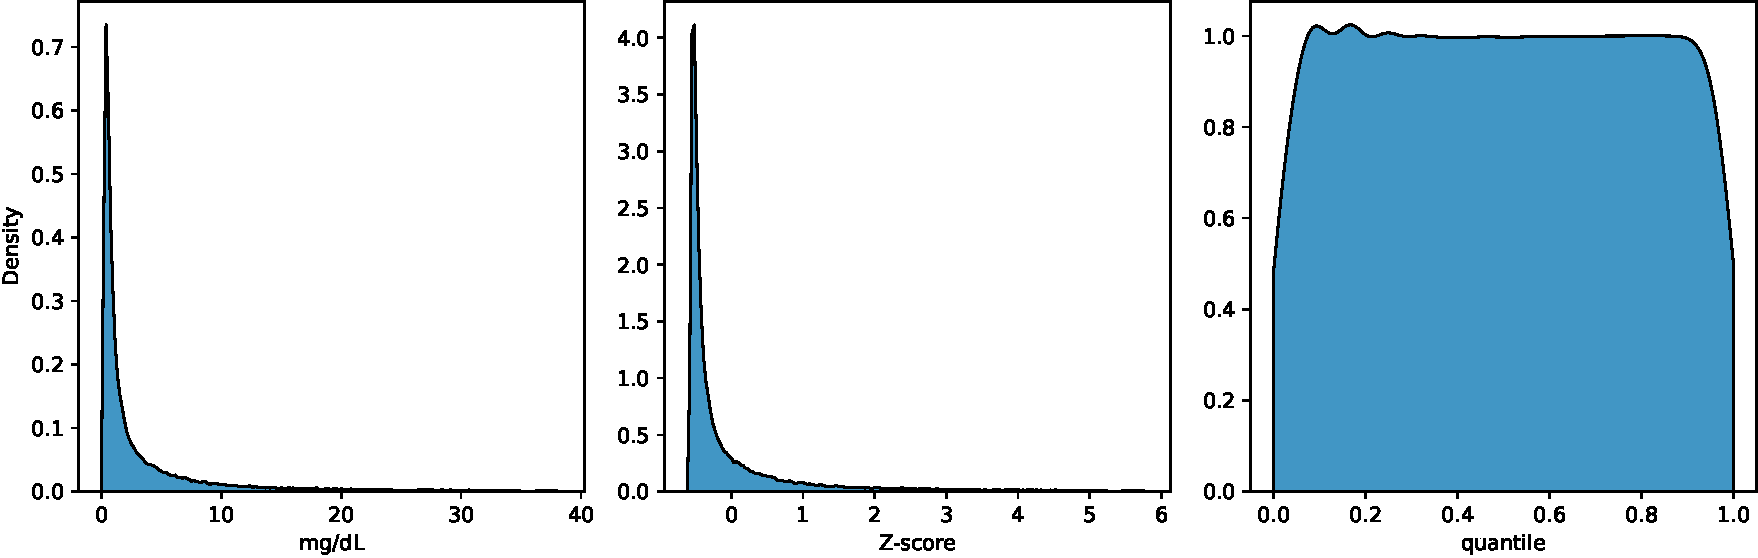
\includegraphics[width=\textwidth]{./figures/transforms_Bilirubin__Total_}
    \caption{KDE-plot of Z-score and \gls{ecdf} normalized distribution for the ``Bilirubin (Total)''  feature in the \gls{mimiciii} dataset. The \gls{ecdf} normalization provides a uniform distribution of values.}
    \label{fig:transforms_bilirubin}
\end{figure}



\subsubsection*{Model Architecture Changes}

The transformation to a bounded space between 0 and 1 allows us to use a sigmoid activation function in the forecasting head, which can be beneficial for the model training process by ensuring outputs are within the desired range.

The model is thus defined as follows:

\[
\mathcal{M}_{\text{ECDF}}(X) = \sigma(\mathcal{M}_{pt}(X)),
\]

where \(\sigma\) is the sigmoid function.

For the fine-tuning phase, we remove the final sigmoid activation layer used during pretraining. We transfer the pretrained model weights and add a single prediction neuron with a sigmoid activation function, following a similar procedure as described in \cref{sec:finetuning}. Thus, the resulting model architecture for a fine-tuning stage is identical to the original model.

\subsubsection*{Additional Considerations for Pretraining Model Evaluation}


\begin{figure}[h!]
    \centering
    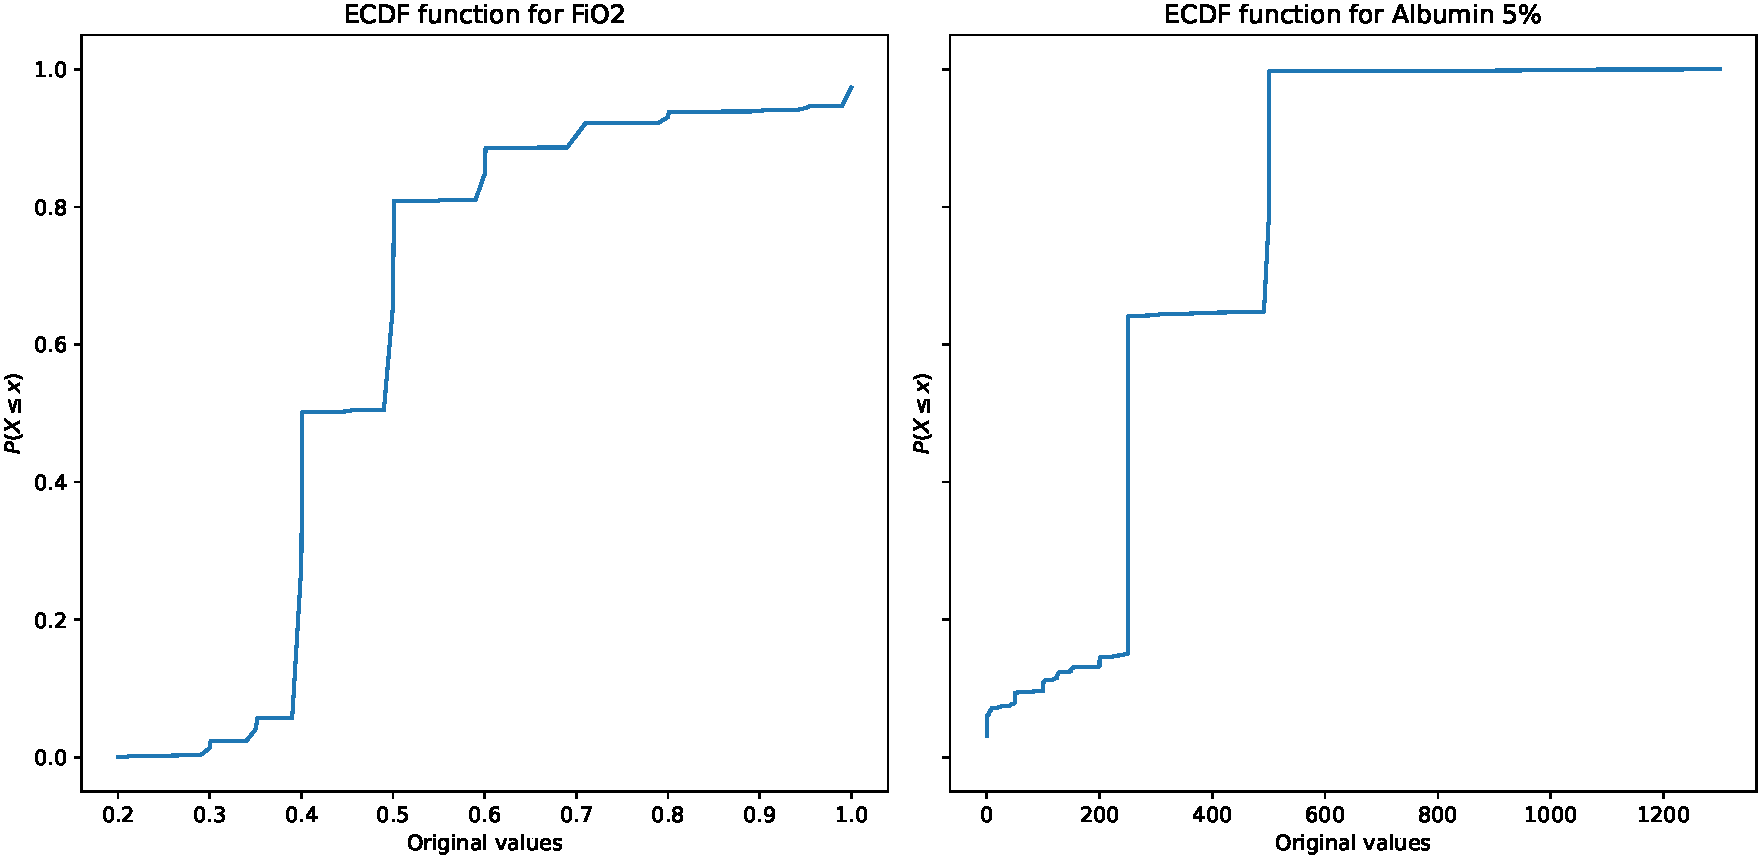
\includegraphics[width=\textwidth]{figures/ecdfs}
    \caption{\gls{ecdf} functions for variables with a low number of unique values, demonstrating the step-like nature of the \gls{ecdf} in such cases.}
    \label{fig:ecdf_pathological}
\end{figure}

When comparing the performance of models using Z-score and \gls{ecdf} normalizations during pretraining, the validation losses cannot be directly compared due to the differing value domains. To enable a fair comparison, we apply inverse transformations to the predicted values to return them to the original data domain. Subsequently, we reapply both Z-score and \gls{ecdf} normalizations to these predicted values and compute the corresponding losses, reported in the ``Z-score'' and ``ECDF'' columns of \cref{tab:normalization_experiments_pretrain}.

For the model trained with \gls{ecdf} normalization, we perform an inverse \gls{ecdf} transformation on its predictions for the test split, converting them back to the original variable domain. This allows us to compute the Z-score normalized values for both the true and predicted data, after which we can calculate the Mean Squared and Absolute errors in Z-score domain.

Conversely, for the model trained with Z-score normalization we apply the inverse Z-score transformation to its predictions, followed by the \gls{ecdf} transformation. This maps the predicted values to their corresponding quantiles using the \gls{ecdf}, allowing us to calculate the \gls{ecdf} \gls{mae} and \gls{ecdf} \gls{mse} between the predicted and true quantiles.

However, the step-function nature of the \gls{ecdf} presents challenges, particularly for variables with a limited number of unique values. Since the \gls{ecdf} increases by a step size \( s = \frac{n_v}{N} \) at each observed value \( v \), where \( N \) is the total number of data points and \( n_v \) is the frequency of \( v \), it may not adequately represent such variables. Discrete measurements like ``Albumin 5\%'' or low-precision variables such as ``FiO2'', which ranges from \num{0} to \num{1} in increments of \num{0.1}, are not well captured by the step-function nature of the \gls{ecdf}. The \gls{ecdf} functions for these cases are shown in \cref{fig:ecdf_pathological}.

Therefore, using the \gls{ecdf} directly for the inverse transformation can lead to inaccuracies. If the predicted value \( \hat{y} \) falls within the same step as the true value \( y \), the difference \( F(\hat{y}) - F(y) \) becomes zero, underestimating the error. Conversely, if the test dataset contains values not observed during training, the inverse transformation may overestimate the error, as those values cannot be accurately recovered from the model's predictions.

To address these issues and achieve a smoother transformation, we apply linear interpolation to \gls{ecdf}. This approach provides a continuous and monotonically increasing function, allowing for a more accurate transformation of predicted values, including those not present in the training dataset.

Given a sorted sequence of values \( V = \{v_1, v_2, \dots, v_N\} \) and their corresponding \gls{ecdf} values \( F(v_i) \), the interpolated \gls{ecdf} \( F(v) \) for any \( v \) between \( v_i \) and \( v_{i+1} \) is estimated as:

\[
F(v) = F(v_i) + \left( \frac{F(v_{i+1}) - F(v_i)}{v_{i+1} - v_i} \right) (v - v_i).
\]

This interpolation mitigates the limitations caused by the discrete nature of the \gls{ecdf} for variables with a limited number of unique values, ensuring more accurate error estimation during model evaluation.

\subsubsection*{Experiment Setup}

We conducted the following set of experiments to evaluate the impact of \gls{ecdf} normalization and different loss functions on the model performance:

\begin{itemize}
    \item \textbf{Z-score}: Using Z-score normalization;
    \item \textbf{ECDF}: Using \gls{ecdf} normalization.
\end{itemize}

In each experiment, we pretrain the model using the specified normalization method with identical \gls{mse} loss function, followed by fine-tuning for the downstream task of mortality prediction. We then evaluated the models to determine how these variations affected overall performance, particularly in terms of Mean Absolute and Squared Errors in both transformed data domains.

To improve the pretrained model evaluation, which involves random input window selection, we selected a random \qty{24}{\hour} window from each \gls{icu} stay in the test split \num{50} times and stored the resulted dataset in persistent storage. This approach allowed to reduce variability across test runs, resulting in more accurate and consistent estimates of model performance, ultimately providing a more reliable assessment of expected error. As before, we run the pretraining \num{10} times on all available training data. Then we fine-tune a pretrained model with the lowest validation loss for \num{10} folds on the data fractions from \qtyrange{10}{100}{\percent}.

\subsection{Experiment 3: Assessing Robustness to Noise and Outliers}

The \gls{mse} loss function is known for its sensitivity to large errors, which can cause the model to focus on reducing significant deviations. This characteristic may lead the model to disproportionately prioritize extreme values, potentially at the cost of overall performance for more typical values. In datasets with skewed distributions or outliers, such as clinical measurements that may exhibit extreme values without corresponding clinical significance, the \gls{mse} loss may encourage the model to overfit these rare occurrences.
% We will investigate the MSE by looking at the disttibution of loss

% TODO: "due to smaller magnitude of values" - double check if I actually stated this in the text
To validate our hypothesis about the improved robustness to noise due to the smaller magnitude of values, we conducted experiments designed to assess its performance under increasingly challenging data conditions.

\subsubsection*{Experiment Setup}

\paragraph{Inclusion of Outliers}

We generated new datasets without outlier filtering to obtain real-world data without the removal of outliers. This includes \num{6470} observations that were previously removed (\qty{0.008307}{\percent} of all data) and \num{81\,730} observations that were replaced with the median value (\qty{0.104929}{\percent} of all data), as described in \cref{sec:outlier-processing}.

\paragraph{Noise Injection}

Given the limited presence of outliers in the data and the model's current predictive performance of nearly \qty{90}{\percent} (as will be seen in the upcoming chapter), suggesting that the task may not be very challenging, we introduced additional noise to further assess the model's robustness. Specifically, we added the following types of noise to the dataset:

\begin{itemize}
    \item \qty{25}{\percent}, \qty{50}{\percent}, \qty{75}{\percent} and \qty{100}{\percent} Uniform Noise: We replaced a fraction of the individual observation values with random values drawn from a continuous uniform distribution bounded by each feature's \(f\) minimum and maximum  values observed in the entire dataset.
    \begin{align*}
        & \epsilon_f \sim \mathcal{U}(\min(\mathcal{F}_f), \max(\mathcal{F}_f)); \\
        & v'_f = v_f \cdot (1 - r) + \epsilon_f \cdot r, \\
        & \text{where } r \sim \text{Bernoulli}(p), \quad p \in \left\{\frac{1}{4}, \frac{2}{4}, \frac{3}{4}, 1\right\}.
    \end{align*}
    This type of noise is designed to simulate errors during measurements or data entry, which can occur in busy clinical settings with high workload conditions or attributed to input error in case of self-reported data.
    \item $1\sigma$, $2\sigma$, and $3\sigma$ Gaussian noise: We added Gaussian noise to all observed values, with standard deviations equal to one, two and three times the standard deviation of each feature's distribution \(\ sigma_f \), respectively:
    \begin{align*}
       & \epsilon_f \sim {\mathcal{N}}(0, (n\sigma_f)^{2}), \quad \text{where } n \in \{1, 2, 3\}; \\
       & v'_f = v_f + \epsilon_f.
    \end{align*}

    Consequently, this setup allows us to observe the model's resilience to measurement errors of varying magnitudes, which could represent different levels of clinical variability or measurement precision in real-world scenarios.
\end{itemize}

We expect that as noise levels increase, model performance will degrade, with uniform noise likely posing a greater challenge due to the presence of extreme values and removing the original data. This experiment will assess the model's resilience to such perturbations, providing insights into its robustness in clinical scenarios with potential measurement variability. Throughout this process, the initial patient splits were preserved to ensure that any observed changes in model performance could be attributed solely to the introduced noise and not to variability in the training or validation data.


\subsection{A Note on the \qty{100}{\percent} Noise Experiment}
\label{sec:100_noise}

In the experiment where \qty{100}{\percent} of the observation values \(v_i\) are replaced with noise, the model performance is expected to remain significantly above random chance, which may initially seem surprising. However, this can be explained by considering that the model's input data comprises multiple types of information, including time-series data \(\mathbf{T} = \{(t_i, f_i, v_i)\}_{i=1}^n\) and demographic data \(\mathbf{d} \in \mathbb{R}^D\). Among these, only the observation values \(v_i\) were randomized in the noise experiment, while the other components remained unchanged.

The inclusion of demographic variables, such as gender and, especially, age, holds substantial predictive power and was not randomized, as these variables are not typically subject to noise. Moreover, the presence of certain clinical measurements can signal severe conditions regardless of their specific values. For example, the administration of medications such as ``Epinephrine'' is often associated with cardiac arrest or severe hypotension, while indicators such as ``Norepinephrine,'' ``Dopamine,'' and ``Vasopressin'' suggest septic shock. Similarly, an ``Intubated'' status and ``FiO2'' levels are related to mechanical ventilation.

Additionally, the size of the available feature space and the number of observations recorded within a certain time window may further contribute to the model's predictive power. The model may learn patterns from the timing and frequency of observations or from the presence of specific features, even when the actual values are randomized.


For the \gls{ecdf} transformation, the uniformly distributed noise values are mapped to random values uniformly distributed between 0 and 1. Similarly, for the Z-score transformation, the uniformly distributed values in the range \( [a, b] \) are shifted to have a mean of 0 and scaled by their standard deviation.

The mean and standard deviation of a uniform distribution \( \text{Unif}(a, b) \) are given by:

\[
    \mu = \frac{a + b}{2}, \quad \sigma = \frac{b - a}{\sqrt{12}}.
\]

Applying the Z-score transformation to the uniform distribution yields the following:

\[
    Z(X) = \frac{X - \mu}{\sigma} = \frac{X - \frac{a + b}{2}}{\frac{b - a}{\sqrt{12}}} = \sqrt{12} \left( \frac{X - \frac{a + b}{2}}{b - a} \right).
\]

Since \( X \) follows \( \text{Unif}(a, b) \), the term \( \frac{X - \frac{a + b}{2}}{b - a} \) is uniformly distributed between \(-0.5\) and \(0.5\). Therefore, the transformed variable \( Z(X) \) becomes:

\begin{equation}
    \label{eq:uniform_z_range}
    Z(X) = \sqrt{12} \cdot \text{Unif}(-0.5, 0.5) = \text{Unif}\left( -\frac{\sqrt{3}}{1}, \frac{\sqrt{3}}{1} \right) \approx \text{Unif}(-1.732, 1.732).
\end{equation}

This result shows that the Z-score transformation of uniformly distributed noise results in another uniform distribution over a fixed range, similar to the \gls{ecdf}-transformed noise. Since both normalization methods transform the noise into standardized forms that do not convey meaningful predictive information, the model performance under \qty{100}{\percent} noise is expected to be similar for both methods.


\section{Reproducibility of the research}

All experiment configurations were stored as \texttt{yaml} files and are available in the code repository at \citeurl{thesiscode}. The codebase is structured in a modular way, with separate files for data processing, model training, and evaluation. The orchestration of the Direct Aciclic Graph (DAG) of jobs, including data downloading and processing as well as model pretraining, selection and finetuning, is implemented as a Snakemake workflow, allowing to reproduce all of the experiments with a single \texttt{snakemake} command. We were able to achieve similar results by replicating our experiments on a provided TCSC HPC Cluster, which allowed us to validate the reproducibility of our results. Thanks to Snakemake, we were able to run the experiments in parallel on multiple nodes simultaneously, which significantly reduced the time required to complete the experiments.

Furthermore, the results of the experiments, including all model checkpoints stored in the Weights\&Biases platform, which allows easy access to the training logs, model checkpoints, and evaluation metrics.


\section{Conclusion of Methodology}

In this chapter, we detailed the architecture and training procedures of our proposed model, including the backbone network, pretraining and fine-tuning phases, evaluation metrics, and implementation specifics. We also discussed the baseline methods used for comparison and outlined the experiments designed to assess various aspects of model performance. The methodologies presented lay the groundwork for the results and analysis in the subsequent chapter.




\chapter{Results}
\label{ch:results}

This chapter presents the outcomes of our experiments designed to assess the model's performance under various configurations and data conditions relevant to clinical settings. We evaluate the model's robustness to class imbalance, the impact of different normalization techniques, and its resilience to noise, with a particular focus on how these factors affect predictive accuracy and calibration.

We begin by comparing baseline models to validate our implementation and ensure alignment with previously published results. Subsequently, we assess the impact of class rebalancing and gradient clipping on the model's calibration and probability estimates, helping identify optimal configurations for model stability and accurate probability predictions. Next, we explore the effects of \gls{ecdf} normalization compared to Z-score normalization in terms of value forecasting and mortality prediction. This examination reveals the benefits and trade-offs associated with each normalization method. Finally, we evaluate the model's resilience to Gaussian and uniform noise. By comparing performance metrics under different noise conditions, we assess how each normalization method performs in the presence of outliers and noise typical for clinical data.

Throughout this chapter, results are reported as averages over 10 runs with standard errors of the mean (\( \text{Mean} \pm \text{SE} \)). In the tables, the relative differences from the baseline, indicated by the underlined text, is provided as the signed percentage change. The percentage change is calculated as follows: $\frac{X - X_{baseline}}{X_{baseline}} \times 100\%$, where $X$ is the performance metric of the given experiment and $X_{baseline}$ is the performance metric of the baseline. Arrows (\textuparrow~ and \textdownarrow) are used to indicate the desired direction of change for each metric (``higher is better'' and ``lower is better'' respectively). Figures illustrate average performance with error bands representing the standard error of the mean.


\section{Baseline models comparison}
\label{sec:baseline_models_comparison}

As shown in \cref{fig:baseline_results}, the \citefield{STraTS2022}{shorttitle} model exhibits superior performance over other baselines, which is consistent with the original paper results. Additionally, our implementation achieves comparable and even slightly improved predictive performance (up to \qty{5}{\percent} higher on \gls{aucpr}) across all data fractions, indicating that our modifications did not compromise the predictive capabilities of the model.


\begin{table}
\begin{tabular}{p{1.5cm}lccc}
\toprule
Data fraction &   & ROC-AUC \textuparrow & AUC-PR \textuparrow & min(Re,Pr) \textuparrow   \\
\midrule
\multirow[t]{6}{*}{10\%} & \underline{STraTS} & 0.878\(\pm\)0.001 & 0.532\(\pm\)0.002 & 0.515\(\pm\)0.004 \\
 & GRU & 0.855\(\pm\)0.002 \(-3\%\) & 0.476\(\pm\)0.005 \(-11\%\) & 0.473\(\pm\)0.002 \(-8\%\) \\
 & SAND & 0.844\(\pm\)0.004 \(-4\%\) & 0.463\(\pm\)0.008 \(-13\%\) & 0.462\(\pm\)0.006 \(-10\%\) \\
 & GRU-D & 0.860\(\pm\)0.003 \(-2\%\) & 0.484\(\pm\)0.006 \(-9\%\) & 0.482\(\pm\)0.006 \(-6\%\) \\
 & TCN & 0.838\(\pm\)0.007 \(-5\%\) & 0.446\(\pm\)0.011 \(-16\%\) & 0.458\(\pm\)0.007 \(-11\%\) \\
 & Ours & \textbf{0.884\(\pm\)0.001 \(+1\%\)} & \textbf{0.556\(\pm\)0.003 \(+5\%\)} & \textbf{0.530\(\pm\)0.002 \(+3\%\)} \\
\cline{1-5}
\multirow[t]{6}{*}{50\%} & \underline{STraTS} & 0.891\(\pm\)0.000 & 0.571\(\pm\)0.002 & 0.539\(\pm\)0.002 \\
 & GRU & 0.880\(\pm\)0.002 \(-1\%\) & 0.543\(\pm\)0.004 \(-5\%\) & 0.519\(\pm\)0.003 \(-4\%\) \\
 & SAND & 0.873\(\pm\)0.002 \(-2\%\) & 0.525\(\pm\)0.004 \(-8\%\) & 0.510\(\pm\)0.003 \(-5\%\) \\
 & GRU-D & 0.885\(\pm\)0.002 \(-1\%\) & 0.548\(\pm\)0.004 \(-4\%\) & 0.530\(\pm\)0.004 \(-2\%\) \\
 & TCN & 0.869\(\pm\)0.002 \(-2\%\) & 0.515\(\pm\)0.004 \(-10\%\) & 0.506\(\pm\)0.003 \(-6\%\) \\
 & Ours & \textbf{0.898\(\pm\)0.000 \(+1\%\)} & \textbf{0.596\(\pm\)0.001 \(+4\%\)} & \textbf{0.553\(\pm\)0.001 \(+3\%\)} \\
\cline{1-5}
\multirow[t]{6}{*}{100\%} & \underline{STraTS} & 0.896\(\pm\)0.000 & 0.589\(\pm\)0.001 & \textbf{0.554\(\pm\)0.001} \\
 & GRU & 0.886\(\pm\)0.001 \(-1\%\) & 0.558\(\pm\)0.002 \(-5\%\) & 0.532\(\pm\)0.002 \(-4\%\) \\
 & SAND & 0.879\(\pm\)0.000 \(-2\%\) & 0.548\(\pm\)0.002 \(-7\%\) & 0.527\(\pm\)0.002 \(-5\%\) \\
 & GRU-D & 0.889\(\pm\)0.001 \(-1\%\) & 0.567\(\pm\)0.002 \(-4\%\) & 0.540\(\pm\)0.002 \(-3\%\) \\
 & TCN & 0.876\(\pm\)0.001 \(-2\%\) & 0.535\(\pm\)0.002 \(-9\%\) & 0.524\(\pm\)0.003 \(-5\%\) \\
 & Ours & \textbf{0.898\(\pm\)0.000 \(+0\%\)} & \textbf{0.599\(\pm\)0.001 \(+2\%\)} & 0.553\(\pm\)0.001 \(-0\%\) \\
\cline{1-5}
\bottomrule
\end{tabular}

\caption{Coparison of baseline models on mortality prediction performance for different percentages of labeled data averaged over 10 runs.}
\label{tab:baseline_experiments}
\end{table}


\begin{figure}
    \centering
    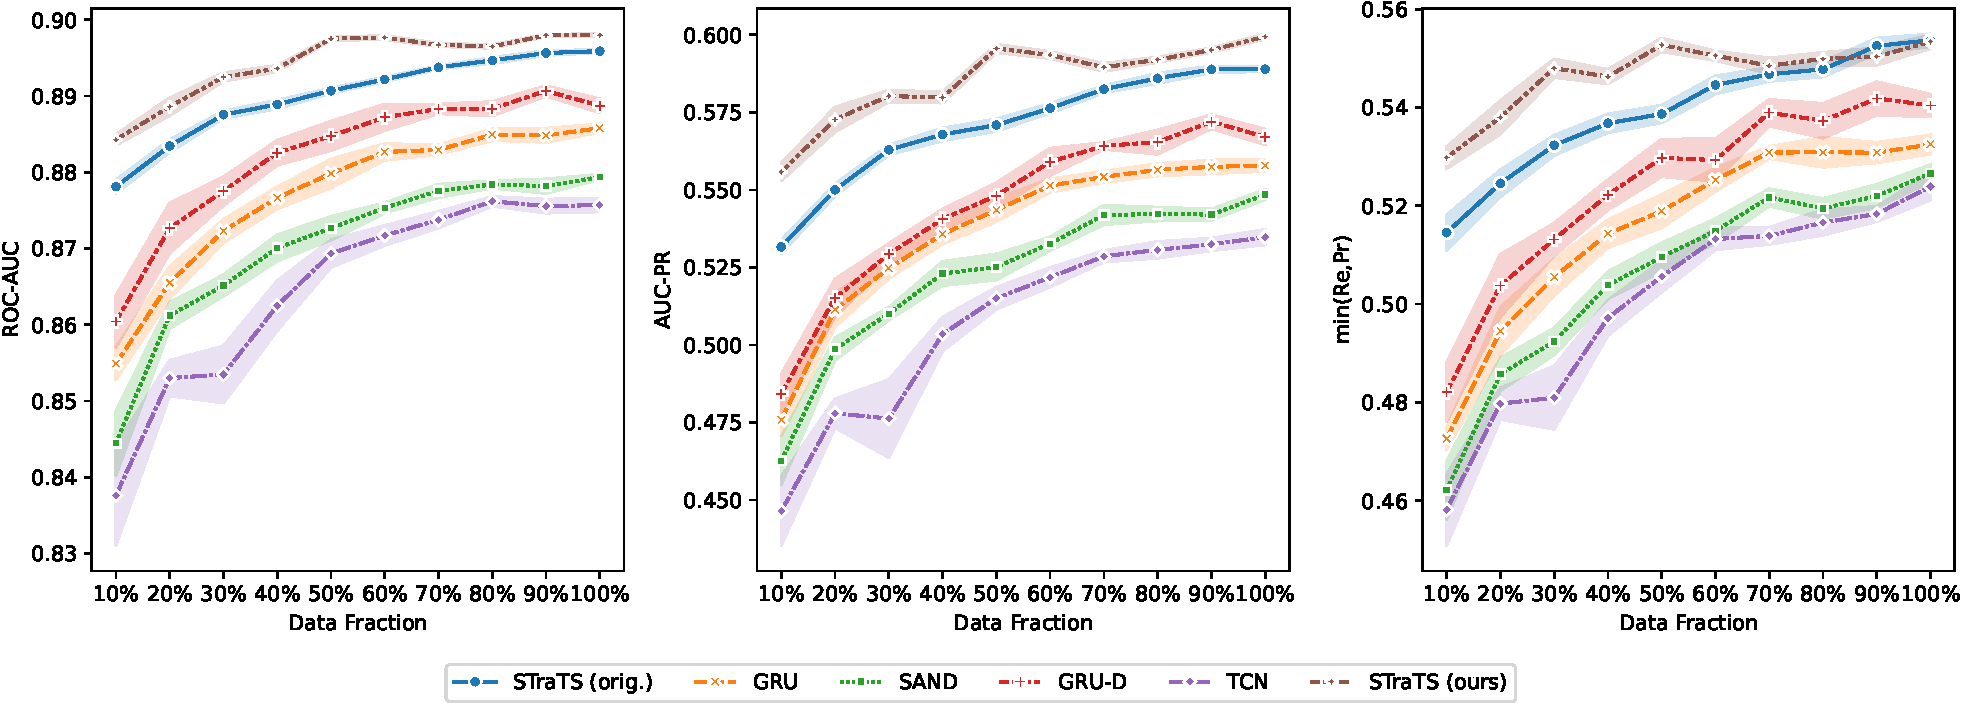
\includegraphics[width=\textwidth]{./figures/baseline_results}
    \caption{Mortality prediction performance of selected baseline models for different percentages of labeled data.}
    \label{fig:baseline_results}
\end{figure}


\section{Performance gains}

\label{sec:performance_gains}
%The  improvements mentioned in \cref{sec:implementation_details} allowed to significantly speedup the training process of the model, reducing the training time from \qty{24.081882(2.171039)}{\minute} and \qty{75.794389(3.999913)}{\minute} to \qty{0.812009(0.11482)}{\minute} and \qty{3.142936(0.25763)}{\minute} for 0.1 and 0.5 training data fractions, respectively compared to the original implementation taken from paper's GitHub. Thit is a speedup of \num{29.65716144}x and \num{24.11579141}x, respectively, compared to the original implementation.

The improvements mentioned in \cref{sec:implementation_details} allowed to significantly speedup the training process of the model, reducing the training time from \qty{24(2)}{\minute} and \qty{76(4)}{\minute} to \qty{0.8(0.1)}{\minute} and \qty{3(0.3)}{\minute} for \qty{10}{\percent} and \qty{50}{\percent} training data fractions, respectively compared to the original implementation taken from paper's GitHub. This is a speedup of \num{30}x and \num{24}x, respectively, compared to the original implementation.



\section{Results 1: Impact of Class Rebalancing and Gradient Clipping}

In addition to the previously used metrics, we estimated the mean predicted mortality risc score and compared it to the true mortality rate in the test dataset (\num{\SupervisedTestDeathPrevalence}), as described in \cref{eq:mre}. The results are presented in \cref{tab:experiment_balancing}, under the Mean Relative Error (MRE) column.

\begin{table}[h]
    \centering
    \begin{tabular}{p{1.5cm}lcccc}
\toprule
Data fraction &   & ROC-AUC \textuparrow & AUC-PR \textuparrow & min(Re,Pr) \textuparrow & MRE \textbar \textdownarrow \textbar   \\
\midrule
\multirow[t]{5}{*}{10\%} & $\beta_{16}$ & \textbf{0.885\(\pm\)0.001} & 0.553\(\pm\)0.003 & 0.529\(\pm\)0.003 & -17.3\% \\
 & $\beta_{16} + os$ & 0.884\(\pm\)0.001 & 0.544\(\pm\)0.005 & 0.524\(\pm\)0.004 & +150.5\% \\
 & $\beta_{16} + w + c$ & 0.884\(\pm\)0.001 & 0.556\(\pm\)0.003 & \textbf{0.530\(\pm\)0.002} & -21.0\% \\
 & $\beta_{4} + w + c$ & 0.875\(\pm\)0.002 & 0.549\(\pm\)0.002 & 0.524\(\pm\)0.003 & -59.5\% \\
 & $\beta_{4} + w$ & \textbf{0.885\(\pm\)0.001} & \textbf{0.559\(\pm\)0.004} & 0.527\(\pm\)0.004 & \textbf{-13.1\%} \\
\cline{1-6}
\multirow[t]{5}{*}{50\%} & $\beta_{16}$ & 0.895\(\pm\)0.000 & 0.584\(\pm\)0.002 & 0.546\(\pm\)0.002 & -16.7\% \\
 & $\beta_{16} + os$ & 0.895\(\pm\)0.000 & 0.580\(\pm\)0.002 & 0.549\(\pm\)0.002 & +140.0\% \\
 & $\beta_{16} + w + c$ & \textbf{0.898\(\pm\)0.000} & \textbf{0.596\(\pm\)0.001} & \textbf{0.553\(\pm\)0.001} & -16.1\% \\
 & $\beta_{4} + w + c$ & 0.893\(\pm\)0.000 & 0.586\(\pm\)0.001 & 0.549\(\pm\)0.002 & -55.5\% \\
 & $\beta_{4} + w$ & 0.895\(\pm\)0.001 & 0.585\(\pm\)0.002 & 0.546\(\pm\)0.001 & \textbf{-11.1\%} \\
\cline{1-6}
\multirow[t]{5}{*}{100\%} & $\beta_{16}$ & \textbf{0.899\(\pm\)0.000} & 0.597\(\pm\)0.001 & 0.551\(\pm\)0.002 & \textbf{-11.5\%} \\
 & $\beta_{16} + os$ & 0.898\(\pm\)0.000 & 0.593\(\pm\)0.001 & 0.548\(\pm\)0.002 & +137.9\% \\
 & $\beta_{16} + w + c$ & 0.898\(\pm\)0.000 & \textbf{0.599\(\pm\)0.001} & \textbf{0.553\(\pm\)0.001} & -20.4\% \\
 & $\beta_{4} + w + c$ & 0.894\(\pm\)0.000 & 0.595\(\pm\)0.001 & 0.548\(\pm\)0.001 & -58.1\% \\
 & $\beta_{4} + w$ & \textbf{0.899\(\pm\)0.000} & 0.597\(\pm\)0.001 & 0.552\(\pm\)0.002 & -11.8\% \\
\cline{1-6}
\bottomrule
\end{tabular}

    \caption{Performance metrics for different class balancing strategies. \\
    Notations are as follows: \emph{w} indicates \gls{wbce} loss; \emph{c} indicates gradient clipping; $\beta_{4}$ and $\beta_{16}$ denote batch sizes; \emph{os} indicates oversampling to achieve class balance.
    }
    \label{tab:experiment_balancing}
\end{table}

To further explore the cause of the discrepancy between the predicted and actual positive class probabilities, we inspected the distribution of predicted risk scores for the positive and negative classes as shown in \cref{fig:risk_score_distributions}.

In the experiment with class rebalancing ($\beta_{16}+os$), the average predicted probability of the positive class is more than two times higher than the true mortality rate. This effect is more pronounced with smaller data fractions, reaching MRE of \qty{+150}{\percent}, and slightly decreasing to \qty{+138}{\percent} with larger amounts of data. Further analysis of the predicted risk score distributions shows that the $\beta_{16}+os$ experiment demonstrates the best separation between the positive and negative classes; however, it is also the most biased towards predicting the positive class for observations that actually belong to the negative class. As can be seen in the upper right plot of \cref{fig:risk_score_distributions}, the area of high (\( \hat{y} > 0.5 \)) risk scores is dominated by samples from negative class, indicating that the model often predicts high risk scores for this population.

Using a smaller batch size with gradient clipping (experiment $\beta_{4} + w + c$) results in the average predicted probability of the positive class being significantly lower than the true mortality rate (MRE from \qtyrange{-59}{-55}{\percent}). Across all reported data fractions, the average predicted risk score is more than twice as small as the actual prevalence, indicating that the model underestimates the risk. As shown in \cref{fig:risk_score_distributions}, the model tends to predict risk scores clustered near 0 and 1, suggesting high confidence in its predictions. However, a majority of the positive class predictions are concentrated around 0, leading to overly confident negative predictions for mortality. Meanwhile, the experiment without gradient clipping (experiment $\beta_{4} + w$) does not exhibit the same behavior as the model with gradient clipping under small batch sizes.

\begin{figure}
    \centering
    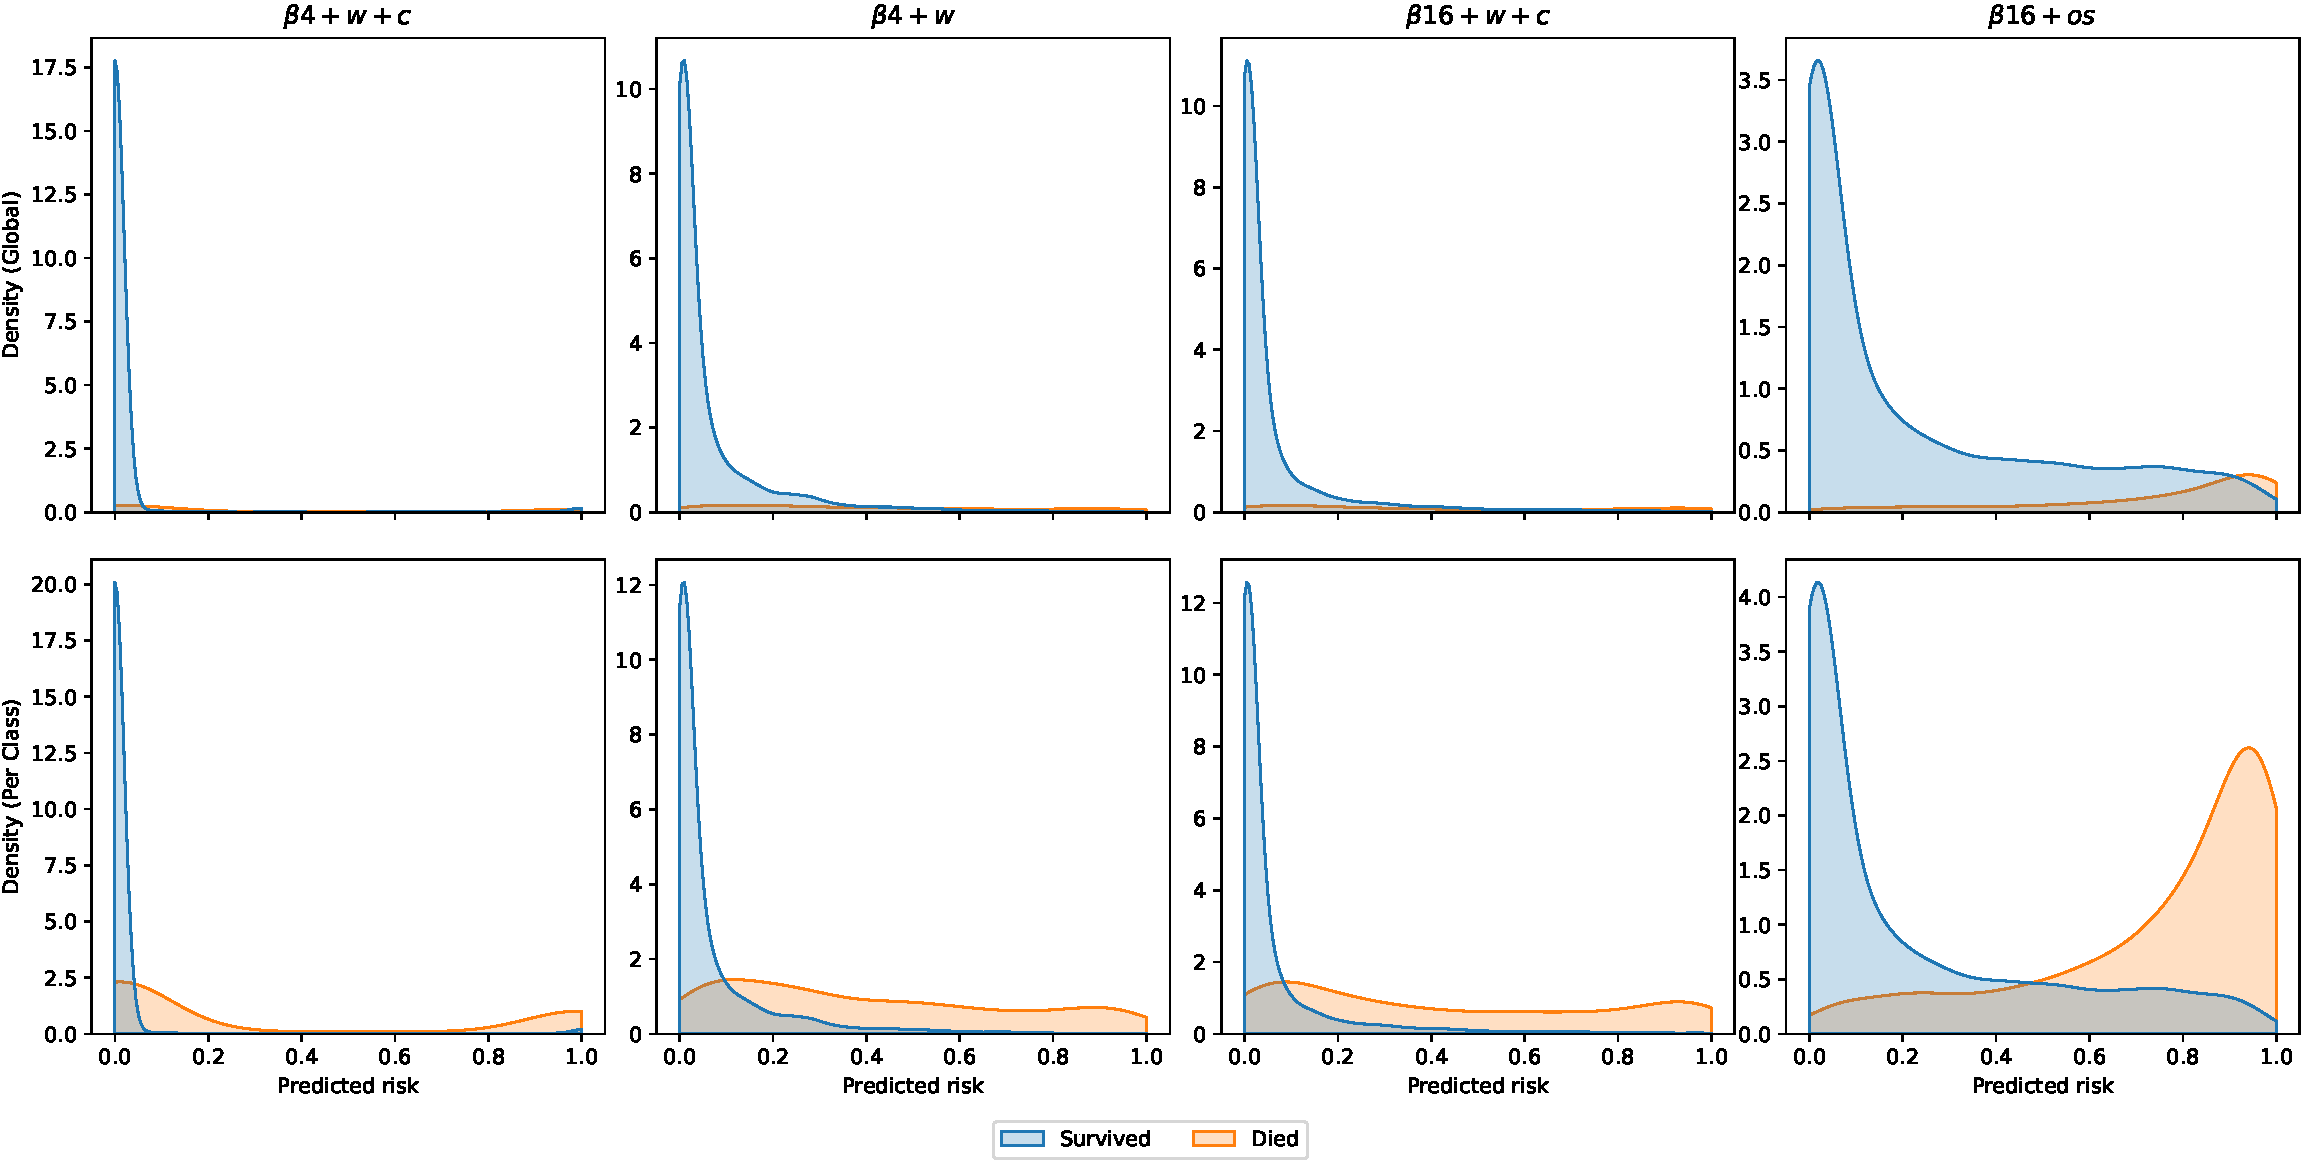
\includegraphics[width=\textwidth]{./figures/risk_score_distributions}
    \caption{Distribution of predicted risk scores for the positive and negative classes.
    In the upper row the combined area under both curves is normalized to 1, highlighting the relative frequency of predictions for each class.
    In the lower row the area under each curve is normalized to 1, allowing comparison of the probability density functions for each class independently. \\
    Notations are as follows: \emph{w} indicates \gls{wbce} loss; \emph{c} indicates gradient clipping; $\beta_{4}$ and $\beta_{16}$ denote batch sizes; \emph{os} indicates oversampling to achieve class balance.}
    \label{fig:risk_score_distributions}
\end{figure}

\paragraph{Considerations for the following experiments}

This analysis indicates that a batch size of \(16\) is sufficient for maintaining robust model performance, achieving the highest \gls{minrp} across all data fractions while consistently maintaining high \gls{auroc} and \gls{aucpr}. Class rebalancing, while useful, risks overestimating mortality probability. Therefore, in subsequent experiments, we will employ a batch size of \(16\) and favor \gls{wbce} loss over class rebalancing, which is consistent with the original setting. Although gradient clipping showed low impact in this experiment, it is expected to play a crucial role in experiments involving datasets with a higher incidence of extreme values. This approach will help maintain model stability and prevent exploding gradients, as confirmed by our observations of gradient magnitudes in the W\&B Dashboard. While MRE values will be monitored in future runs to ensure model calibration, they will not be reported unless they significantly deviate from \num{0}.


\section{Results 2: Impact of ECDF Normalization}

In this section we analyzed the pretraining losses and fine-tuning metrics of models using both methods to assess the effectiveness of \gls{ecdf} normalization compared to Z-score normalization.


\subsection{Pretraining Losses}

The results, presented in \cref{tab:normalization_experiments_pretrain}, detail the \gls{mse} and \gls{mae} in both the Z-score (Z) and \gls{ecdf} (E) domains achieved on a time series forecasting. The ``Z'' losses reflect the model's precision in predicting the number of standard deviations from the mean, while the ``E'' losses indicate the accuracy in predicting the percentile rank of the observation values.

\begin{table}
\begin{tabular}{lcccc}
\toprule
  & Z MSE $\times 10^3$ \textdownarrow & Z MAE $\times 10^3$ \textdownarrow & E MSE $\times 10^3$ \textdownarrow & E MAE $\times 10^3$ \textdownarrow   \\
\midrule
\underline{Z-score} & \textbf{363.5\(\pm\)1.3} & 361.7\(\pm\)0.9 & 39.6\(\pm\)0.2 & 138.9\(\pm\)0.4 \\
ECDF & 383.6\(\pm\)1.2 \(+6\%\) & \textbf{335.8\(\pm\)0.8 \(-7\%\)} & \textbf{27.2\(\pm\)0.1 \(-31\%\)} & \textbf{118.3\(\pm\)0.3 \(-15\%\)} \\
\bottomrule
\end{tabular}

\caption{Pretrain losses for \gls{ecdf} and Z-score normalization experiments. E stands for \gls{ecdf} (percentile domain) and Z for Z-score domain. \gls{mse} and \gls{mae} are the mean squared error and mean absolute error, respectively.}
\label{tab:normalization_experiments_pretrain}
\end{table}


The first row of the table corresponds to the Z-score normalization, achieving a \gls{mse} of \num{0.3635} in the Z-score domain. The \gls{ecdf} normalization, shown in the second row, results in a \qty{6}{\percent} increase in Z \gls{mse} of \num{0.3836}, which is expected as this metric was not directly optimized for the \gls{ecdf} model. However, the \gls{ecdf} model demonstrates a \qty{7}{\percent} reduction in Z \gls{mae}, suggesting that, on average, the absolute error, measured in standard deviations and linearly related to the original scale of the variable, is lower.


When evaluating performance in the percentile domain (E), the \gls{ecdf} normalization model demonstrates significant improvements. Specifically, there is a \qty{31}{\percent} reduction in E \gls{mse} and a \qty{15}{\percent} reduction in E \gls{mae} compared to the Z-score normalization. These results suggest that \gls{ecdf} normalization allows for significantly more precise prediction of the percentiles of observation values.


\subsection{Finetune Metrics}


The fine-tuning metrics presented in \cref{tab:normalization_experiments_finetune} allow for direct comparison between the two normalization techniques, as the binary label prediction is unaffected by the normalization method. Both \gls{ecdf} and Z-score normalization demonstrate comparable performance, with metrics varying by no more than \qty{2}{\percent} across the reported data fractions. Notably, the model achieves \qty{90}{\percent} \gls{auroc} for the first time under \gls{ecdf} normalization, though overall, no clear advantage emerges between the methods.



\begin{table}
\begin{tabular}{p{1.5cm}lccc}
\toprule
Data fraction &   & ROC-AUC \textuparrow & AUC-PR \textuparrow & min(Re,Pr) \textuparrow   \\
\midrule
\multirow[t]{2}{*}{10\%} & \underline{Z-score} & 0.884\(\pm\)0.001 & 0.556\(\pm\)0.003 & \textbf{0.530\(\pm\)0.002} \\
 & ECDF & \textbf{0.886\(\pm\)0.001 \(+0\%\)} & \textbf{0.562\(\pm\)0.004 \(+1\%\)} & 0.527\(\pm\)0.004 \(-1\%\) \\
\cline{1-5}
\multirow[t]{2}{*}{50\%} & \underline{Z-score} & \textbf{0.898\(\pm\)0.000} & \textbf{0.596\(\pm\)0.001} & \textbf{0.553\(\pm\)0.001} \\
 & ECDF & 0.895\(\pm\)0.000 \(-0\%\) & 0.587\(\pm\)0.001 \(-2\%\) & 0.540\(\pm\)0.001 \(-2\%\) \\
\cline{1-5}
\multirow[t]{2}{*}{100\%} & \underline{Z-score} & 0.898\(\pm\)0.000 & \textbf{0.599\(\pm\)0.001} & \textbf{0.553\(\pm\)0.001} \\
 & ECDF & \textbf{0.900\(\pm\)0.000 \(+0\%\)} & 0.598\(\pm\)0.001 \(-0\%\) & 0.549\(\pm\)0.001 \(-1\%\) \\
\cline{1-5}
\bottomrule
\end{tabular}

\caption{Finetune metrics for \gls{ecdf} and Z-score normalization experiments.}
\label{tab:normalization_experiments_finetune}
\end{table}

The metric trends across all data fractions, as illustrated in \cref{fig:gaussian_noise_results,fig:uniform_noise_results} in the following section, show that the predictive performance of both methods intersects and is largely indistinguishable. Metrics from this experiment are highlighted in light gray, providing a baseline for comparison with noise-affected results.


\section{Results 3. Robustness to Noise and Outliers}

This section presents the model's robustness to noise under different normalization techniques. \Cref{fig:gaussian_noise_results} shows the performance under Gaussian noise discussed in \cref{sec:gaussian_noise}, while \cref{fig:uniform_noise_results} presents results with uniform noise examined in \cref{sec:uniform_noise}.



\begin{table}
\begin{tabular}{lccc}
\toprule
  & ROC-AUC \textuparrow & AUC-PR \textuparrow & min(Re,Pr) \textuparrow   \\
\midrule
\underline{Z-score} & 0.898\(\pm\)0.000 & 0.599\(\pm\)0.001 & 0.553\(\pm\)0.001 \\
Z-score $1\sigma$ Gauss & 0.873\(\pm\)0.001 \(-3\%\) & 0.539\(\pm\)0.002 \(-10\%\) & 0.519\(\pm\)0.002 \(-6\%\) \\
Z-score $2\sigma$ Gauss & 0.865\(\pm\)0.000 \(-4\%\) & 0.504\(\pm\)0.001 \(-16\%\) & 0.490\(\pm\)0.001 \(-11\%\) \\
Z-score $3\sigma$ Gauss & 0.852\(\pm\)0.000 \(-5\%\) & 0.479\(\pm\)0.001 \(-20\%\) & 0.473\(\pm\)0.001 \(-14\%\) \\
Z-score 25\% Unif & 0.869\(\pm\)0.000 \(-3\%\) & 0.517\(\pm\)0.001 \(-14\%\) & 0.498\(\pm\)0.002 \(-10\%\) \\
Z-score 50\% Unif & 0.849\(\pm\)0.001 \(-5\%\) & 0.479\(\pm\)0.001 \(-20\%\) & 0.468\(\pm\)0.002 \(-15\%\) \\
Z-score 75\% Unif & 0.838\(\pm\)0.001 \(-7\%\) & 0.446\(\pm\)0.001 \(-26\%\) & 0.449\(\pm\)0.002 \(-19\%\) \\
Z-score 100\% Unif & 0.827\(\pm\)0.001 \(-8\%\) & 0.402\(\pm\)0.003 \(-33\%\) & 0.416\(\pm\)0.002 \(-25\%\) \\
ECDF & 0.900\(\pm\)0.000 \(+0\%\) & 0.598\(\pm\)0.001 \(-0\%\) & 0.549\(\pm\)0.001 \(-1\%\) \\
ECDF $1\sigma$ Gauss & 0.876\(\pm\)0.000 \(-2\%\) & 0.544\(\pm\)0.001 \(-9\%\) & 0.514\(\pm\)0.001 \(-7\%\) \\
ECDF $2\sigma$ Gauss & 0.862\(\pm\)0.000 \(-4\%\) & 0.497\(\pm\)0.001 \(-17\%\) & 0.483\(\pm\)0.001 \(-13\%\) \\
ECDF $3\sigma$ Gauss & 0.849\(\pm\)0.000 \(-5\%\) & 0.479\(\pm\)0.001 \(-20\%\) & 0.475\(\pm\)0.001 \(-14\%\) \\
ECDF 25\% Unif & 0.890\(\pm\)0.000 \(-1\%\) & 0.565\(\pm\)0.001 \(-6\%\) & 0.520\(\pm\)0.001 \(-6\%\) \\
ECDF 50\% Unif & 0.887\(\pm\)0.000 \(-1\%\) & 0.560\(\pm\)0.001 \(-7\%\) & 0.531\(\pm\)0.001 \(-4\%\) \\
ECDF 75\% Unif & 0.857\(\pm\)0.000 \(-5\%\) & 0.484\(\pm\)0.001 \(-19\%\) & 0.478\(\pm\)0.002 \(-14\%\) \\
ECDF 100\% Unif & 0.835\(\pm\)0.001 \(-7\%\) & 0.434\(\pm\)0.002 \(-28\%\) & 0.434\(\pm\)0.002 \(-22\%\) \\
\bottomrule
\end{tabular}

\caption{Performance metrics for different noise levels and normalization methods for \qty{100}{\percent} data fraction.}
\label{tab:noise_experiments}
\end{table}

\subsection{Gaussian Noise}
\label{sec:gaussian_noise}

\begin{figure}
    \centering
    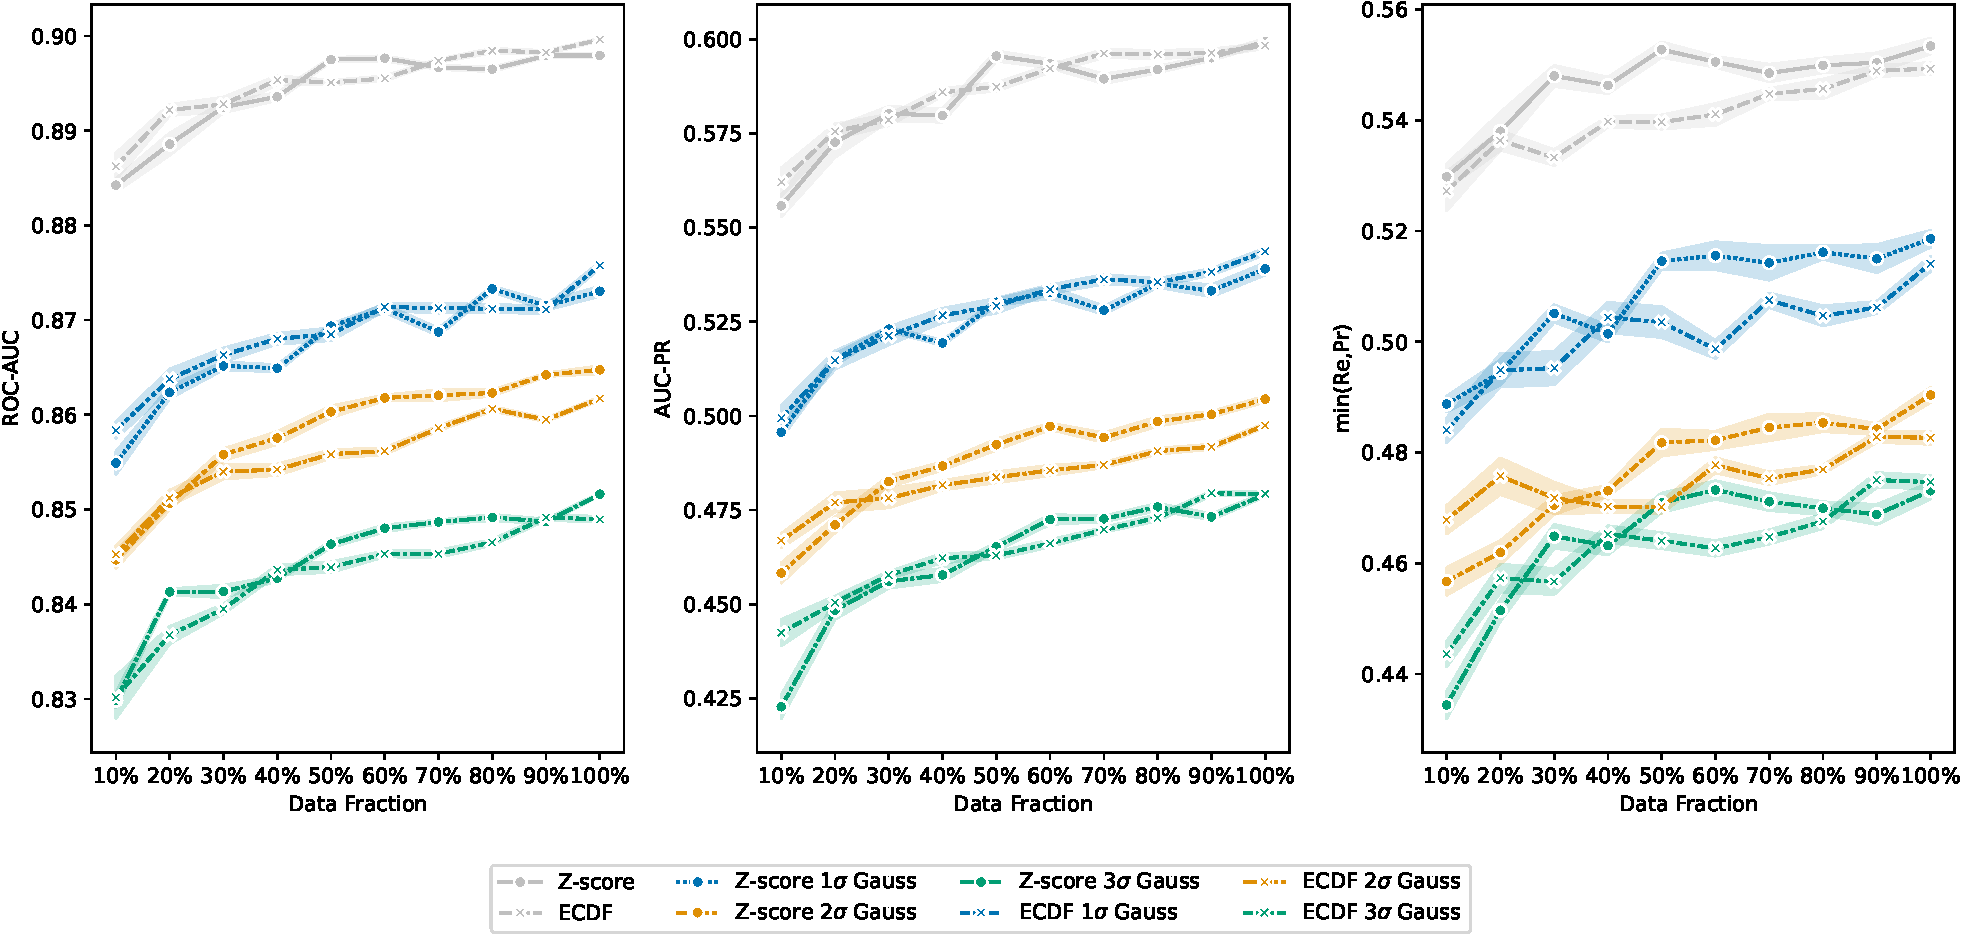
\includegraphics[width=\textwidth]{./figures/gaussian_noise_results}
    \caption{Comparison of performance metrics for mortality prediction under Gaussian noise across varying data fractions. X markers represent \gls{ecdf} normalization, and circles represent Z-score normalization. Lines of the same color correspond to the same noise level.}
    \label{fig:gaussian_noise_results}
\end{figure}


In experiments with Gaussian noise, there was no observable advantage in using \gls{ecdf} normalization over Z-score normalization. Both models, denoted by X markers for \gls{ecdf} and circles for Z-score in \cref{fig:gaussian_noise_results}, show similar performance across all data fractions and noise levels, with overlapping curves indicating similar results for each metric. As expected, increasing the noise level leads to an equivalent decrease in performance for both normalization approaches.

At the highest Gaussian noise level with the full dataset (\qty{100}{\percent} data fraction), model performance, as measured by \gls{auroc}, \gls{aucpr} and \gls{minrp}, dropped by \qty{5}{\percent} \qty{20}{\percent} and \qty{14}{\percent}, respectively, for both normalizations. Detailed results are provided in \cref{tab:noise_experiments}.



\subsection{Uniform Noise}
\label{sec:uniform_noise}

\begin{figure}
    \centering
    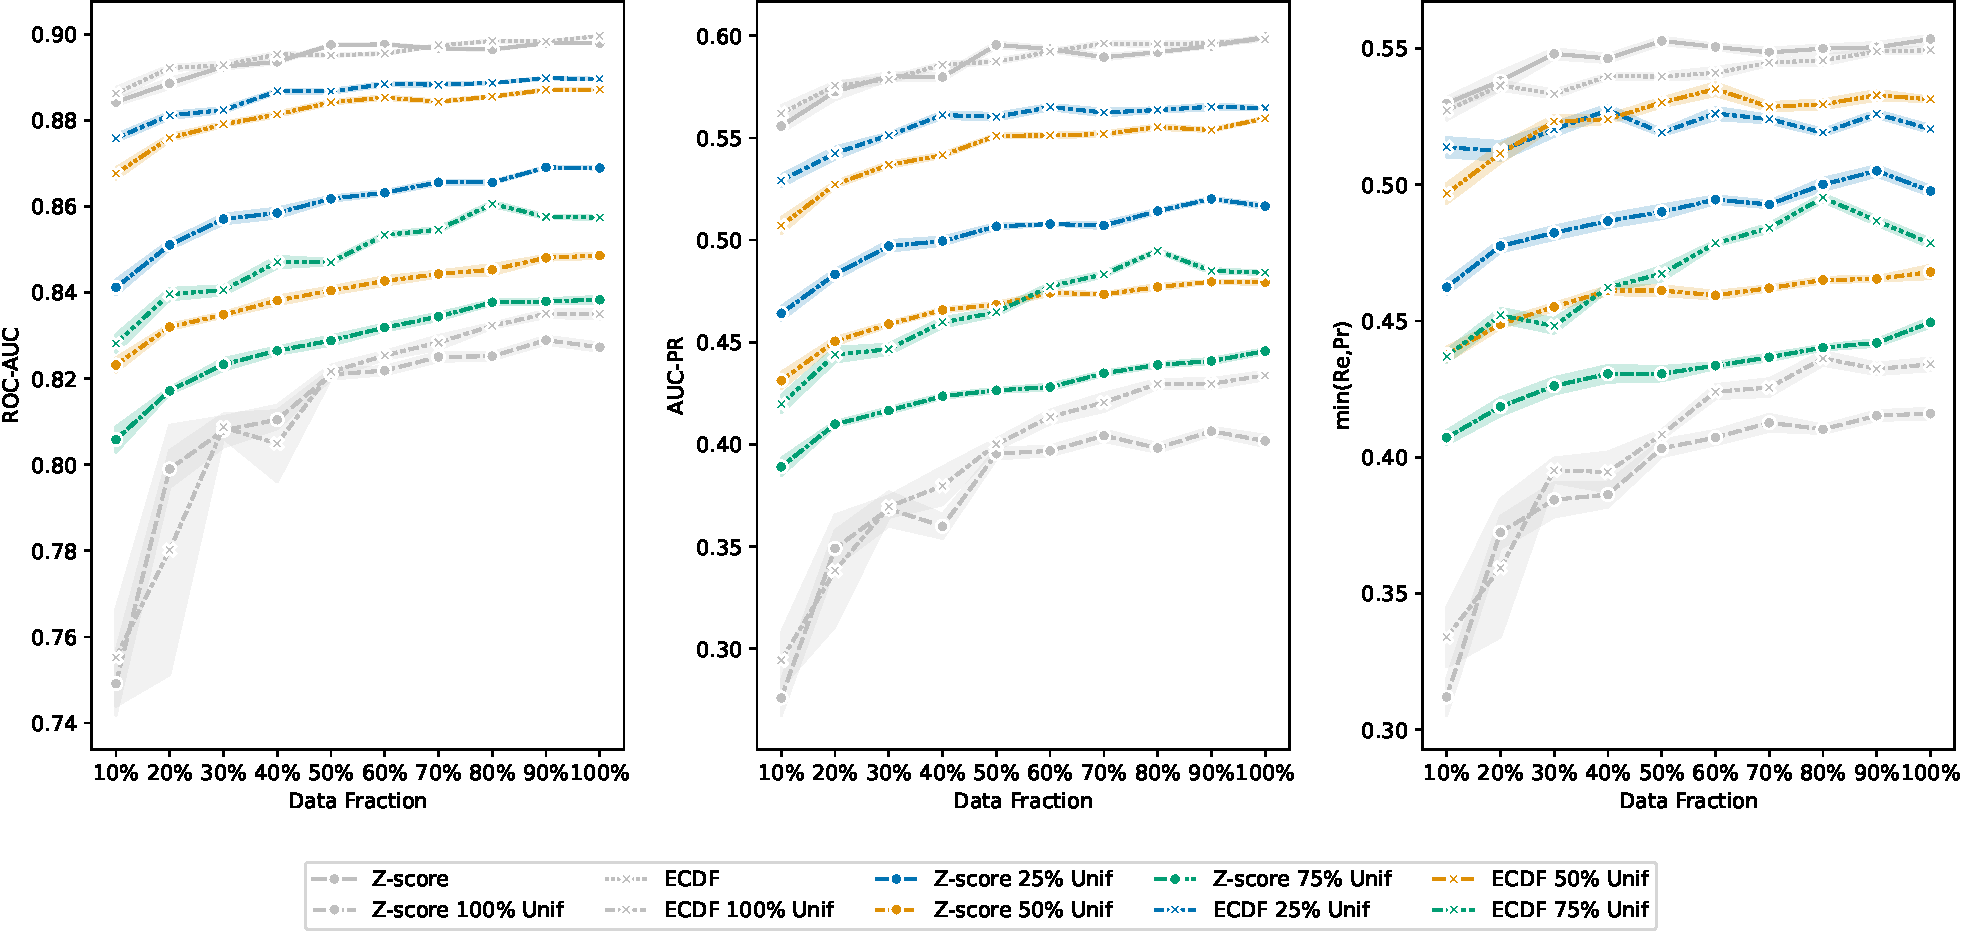
\includegraphics[width=\textwidth]{./figures/uniform_noise_results}
    \caption{Comparison of performance metrics for mortality prediction under uniform noise across varying data fractions. X markers represent \gls{ecdf} normalization, and circles represent Z-score normalization. Lines of the same color correspond to the same noise level.}
    \label{fig:uniform_noise_results}
\end{figure}


In contrast, the results with uniform noise show a clear advantage of \gls{ecdf} normalization in the presence of significant outliers introduced by the broad range of random values. Across all metrics, the performance of the \gls{ecdf}-normalized model consistently outperformed the Z-score normalized model, as indicated in \cref{fig:uniform_noise_results}.

Specifically, with the full dataset and \qty{75}{\percent} uniform noise, predictive performance metrics for Z-score normalization dropped by \qty{7}{\percent} for \gls{auroc}, \qty{26}{\percent} for \gls{aucpr}, and \qty{19}{\percent} for \gls{minrp} relative to noise-free data. In contrast, \gls{ecdf} normalization resulted in smaller reductions in performance, with declines of only \qty{4}{\percent}, \qty{18}{\percent}, and \qty{12}{\percent}, respectively. This suggests that \gls{ecdf} normalization provides greater resilience to extreme noise levels with a large number of outliers. We also observe that in the case of \qty{100}{\percent} noise, both normalization methods demonstrate similar performance, with intersecting error bands. This outcome aligns with our theoretical expectations discussed in \cref{sec:100_noise}.

However, directly comparing \gls{auroc} by percentage change can be misleading because the minimal reasonable performance starts from \(0.5\), representing random guessing. This limits the meaningful range for comparison and can exaggerate the perceived impact of changes. Furthermore, factors such as the model architecture's intrinsic robustness to outliers and the influence of demographic data, which were not affected by the added noise, can overshadow the effects of noise on other variables. For instance, the fusion attention module can inherently mitigate the influence of outliers by assigning them lower attention scores (see \cref{sec:fusion_self_attention}).


To more objectively analyze the effect of the normalization methods while minimizing the influence of these confounding factors, we propose reframing the analysis by examining how much of the model performance is retained relative to the extremes of completely noise-free data and entirely noisy data. We apply Min-Max scaling to the performance metrics, normalizing the results between the lowest achieved performance (average of experiments with complete noise) and the highest (average of experiments with pure data). We refer to these rescaled metrics as \textit{retained} predictive performance, where \qty{100}{\percent} represents the model's performance on noise-free data, and \qty{0}{\percent} represents performance when all observations are replaced with noise.


It is important to note that the analysis presented here may not adhere strictly to conventional statistical methodologies and may not be fully rigorous from a mathematical standpoint. Rather, it offers a new perspective aimed at isolating and comparing the effects of normalization methods independently of other factors influencing the model performance, providing insight into the specific impact of \gls{ecdf} and Z-score normalization on noise resilience.


\begin{table}
\begin{tabular}{p{1cm}p{1.2cm}ccc}
\toprule
Noise level &  & $\overline{\text{ROC-AUC}}$ \textuparrow & $\overline{\text{AUC-PR}}$ \textuparrow & $\overline{\text{min(Re,Pr)}}$ \textuparrow  \\
\midrule
 & \underline{Z-score} & 0.575\(\pm\)0.004 & 0.568\(\pm\)0.006 & 0.593\(\pm\)0.013 \\
\multirow[t]{2}{*}{25.0\%} & ECDF & \textbf{0.869\(\pm\)0.003 \(+51\%\)} & \textbf{0.820\(\pm\)0.004 \(+44\%\)} & \textbf{0.765\(\pm\)0.010 \(+29\%\)} \\
\cline{1-5}
 & \underline{Z-score} & 0.285\(\pm\)0.009 & 0.372\(\pm\)0.007 & 0.368\(\pm\)0.019 \\
\multirow[t]{2}{*}{50.0\%} & ECDF & \textbf{0.834\(\pm\)0.002 \(+193\%\)} & \textbf{0.794\(\pm\)0.003 \(+113\%\)} & \textbf{0.848\(\pm\)0.006 \(+130\%\)} \\
\cline{1-5}
 & \underline{Z-score} & 0.139\(\pm\)0.011 & 0.196\(\pm\)0.006 & 0.228\(\pm\)0.013 \\
\multirow[t]{2}{*}{75.0\%} & ECDF & \textbf{0.411\(\pm\)0.006 \(+196\%\)} & \textbf{0.397\(\pm\)0.004 \(+103\%\)} & \textbf{0.447\(\pm\)0.012 \(+96\%\)} \\
\cline{1-5}
\bottomrule
\end{tabular}

\caption{Retained mortality prediction performance on different metrics under uniform noise with \qty{100}{\percent} data fraction.}
\label{tab:noise_experiments_rescaled}
\end{table}

The results in \cref{tab:noise_experiments_rescaled} illustrate that \gls{ecdf} normalization substantially enhances resilience to uniform noise across all levels. Notably, under \qty{50}{\percent} noise, \gls{ecdf} normalization outperforms Z-score normalization demonstrating \qty{193}{\percent} higher retained \gls{auroc} and \qty{130}{\percent} higher retained \gls{minrp}.

Another noticeable trend is the relationship between the fraction of added noise and the retained performance. \gls{ecdf} normalization demonstrates a less-than-proportional decrease in performance as noise increases. For example, with a \qty{50}{\percent} noise level, the retained \gls{auroc}, \gls{aucpr}, and \gls{minrp} for \gls{ecdf} normalization are \qty{83}{\percent}, \qty{79}{\percent}, and \qty{85}{\percent}, respectively. This indicates that \gls{ecdf} normalization effectively mitigates the impact of noise. In contrast, Z-score normalization shows a greater-than-proportional decrease in performance under the same noise level, specifically \qty{29}{\percent}, \qty{37}{\percent}, and \qty{37}{\percent}, respectively. In fact, the retained performance of Z-score normalization drops nearly by half at just \qty{25}{\percent} noise level.

This trend persists even as noise levels increase. Under \qty{75}{\percent} noise, \gls{ecdf} normalization retains nearly triple the \gls{auroc} retention compared to Z-score normalization, and nearly double the retention of \gls{aucpr} and \gls{minrp}. These findings emphasize \gls{ecdf} normalization's robustness, particularly in handling high levels of noise and outliers, where it consistently sustains predictive performance.


\section{Chapter Conclusion}

In this chapter, we evaluated the performance of various experimental settings in the mortality prediction and time series forecasting, focusing on class balancing strategies, data normalization techniques, and robustness to noise. The \citefield{STraTS2022}{shorttitle} model, with implementation improvements, demonstrated superior performance, confirming its suitability as the foundation for further experimentation.

The introduction of \gls{ecdf} normalization showed promising results, especially in handling percentile-based predictions. This approach provided comparable fine-tuning performance metrics to Z-score normalization, though with enhanced resilience under uniform noise, which produced significant outliers. \gls{ecdf} normalization maintained predictive stability, underscoring its potential in applications with high variance or extreme values.

These results set the stage for an in-depth discussion on the implications of our findings. The next chapter will discuss the impact of observed results, their clinical relevance, and practical application.


\chapter{Discussion}
\label{ch:discussion}

This chapter interprets the key findings from our experiments, positioning them within the broader context of machine learning for healthcare applications. We examine the impact of the implemented model adjustments on performance, efficiency, and robustness. Through comparative analysis with baseline models and exploration of class rebalancing, normalization techniques, and noise robustness, we assess how these modifications enhance the model's utility in clinical settings.


\section{Model Enhancements}

We extended the original analysis by evaluating the performance of the model in data fractions greater than \qty{50}{\percent}, which were not covered in the original paper. Our results confirm that the \citefield{STraTS2022}{shorttitle} model continues to outperform other baselines at these higher data levels, strengthening its predictive robustness.

Furthermore, by disabling weight decay for norm and bias parameters to adhere to best practices and allowing the model to train for an unlimited number of epochs until convergence, we achieved notable improvements (up to \qty{5}{\percent} on \gls{aucpr}) in predictive accuracy on smaller data fractions. These optimizations highlight the importance of refining training configurations to attain optimal model performance.

Improvements in computational efficiency enabled a more rapid experimentation process, allowing up to 30 times faster iterations and contributing to greater environmental sustainability through reduced energy consumption. The decrease in memory requirements also allowed us to explore larger model variants with up to 25 times the original parameter count, which would have been computationally prohibitive with the original implementation.
 Although these larger models were not included in this study, this improved efficiency and scalability underscore the model's applicability to real-world clinical settings, where data complexity and resource constraints often present challenges. By making the model more computationally accessible, these refinements hold promise for more widely applicable and adaptable healthcare predictive models as data availability and computational resources continue to grow.

\section{Balancing the Imbalances}

The findings of our experiments on class balancing underscore the challenges of addressing class imbalance in mortality prediction tasks, where the balance of model calibration and its discrimination ability is crucial.

Our results indicate that weighted loss functions, particularly with a batch size of \(16\), helped to maintain balanced model performance. However, when smaller batch sizes were combined with gradient clipping, there was a tendency to underestimate the positive class probability. This may stem from the frequent absence of positive samples in mini-batches and the reduced effect of class weighting, resulting in gradient steps biased toward predicting the negative class. Notably, this underestimation was not observed with a small batch size without gradient clipping, which showed a minimal discrepancy between the mean predicted risk and the true mortality rate. This suggests that gradient clipping, while effective in preventing exploding gradients, can inadvertently constrain positive samples updates in small batch settings, limiting the model’s ability to learn effectively from the minority class.


In contrast, the experiment with a larger batch size did not demonstrate the same behavior, supporting our hypothesis that gradient clipping has a more pronounced effect with smaller batch sizes and class weights. These findings highlight the importance of carefully selecting batch size and gradient clipping parameters to ensure effective learning from minority class examples.


The oversampling approach, while achieving better class separation, resulted in a consistent overestimation of the positive class probability, especially in smaller data fractions. This outcome suggests that oversampling can increase \gls{auroc} scores by improving discrimination, but at the same time negatively affect calibration, leading to overfitting and biasing predictions towards the minority class \cite[][13]{Weiss2004Mining}. Thus, while oversampling may yield better discrimination, it does not necessarily ensure well-calibrated predictions, especially when the model is used for clinical risk scores where accurate probability estimates are required.
% Additional calibration techniques, such as Platt scaling or isotonic regression, may be necessary to correct for these biases.

Despite these issues, the model maintains the ability to rank samples by their predicted probability of the positive class, as indicated by similar \gls{auroc} and \gls{aucpr} values across all experiments. However, the model's predictions are less calibrated with the actual mortality risk, highlighting the importance of evaluating the model's calibration in addition to its discrimination ability when assessing its performance as a risk score.

In summary, addressing class imbalance is complex, particularly when combined with gradient clipping, loss weighting, and small batch sizes. Weighted loss with a batch size of \(16\) provided a good balance of calibration and discrimination, suggesting that weighting alone may be an effective baseline method for similar tasks without introducing the overfitting risks seen with oversampling. Conversely, gradient clipping with small batch sizes may result in underestimating positive class probability, impairing the model’s learning from minority class examples. These findings confirm our initial hypothesis about the interplay between these hyperparameters and underscore the necessity of careful calibration to ensure accurate and reliable predictions.

\section{Impact of ECDF Normalization on Forecasting Performance}
\label{sec:forecasting_performance}

Our findings indicate that \gls{ecdf} normalization enhances the model's ability to predict the relative standing of values within a distribution (i.e., their percentiles), while maintaining comparable performance in the original domain. This approach is particularly beneficial in clinical contexts where the exact numeric value may be less important than its relative position within the population.

For example, in predicting glucose levels, a model using \gls{ecdf} normalization can more accurately place a glucose level prediction in the 95th percentile, which holds meaningful clinical implications. While it may be slightly less precise in terms of squared error in predicting specific high values, such as \qty{300}{\mg\per\deci\liter} and \qty{350}{\mg\per\deci\liter}, both values indicate extreme elevation, making the exact numerical distinction less clinically relevant.

These results suggest that by focusing on percentile ranks, \gls{ecdf} normalization can improve the model's performance in predicting clinically relevant metrics, especially when dealing with skewed data distributions and extreme values.

\section{Impact of ECDF Normalization on Classification Performance}

The fine-tuning metrics indicate minimal differences between the two normalization methods, with performance differing by no more than \qty{2}{\percent}. This finding suggests that \gls{ecdf} normalization does not substantially impact the model's ability to perform on the downstream mortality prediction task when applied to a sanitized dataset from which extreme values have been removed.

\section{Robustness to Noise and Outliers}

The noise robustness experiments reveal that while \gls{ecdf} normalization did not offer an advantage under Gaussian noise conditions, it demonstrated clear benefits when handling uniform noise, particularly in the presence of extreme outliers. In the Gaussian noise experiments (\cref{fig:gaussian_noise_results}), both \gls{ecdf} and Z-score normalization performed similarly, suggesting that Gaussian noise does not challenge model robustness in a way that differentiates between these normalization methods.

Originally, it was anticipated that \gls{ecdf} normalization would yield some improvements across all experiments, partly due to the inclusion of outliers that were initially filtered out. However, the results of the Gaussian noise experiment did not show significant benefits. This may be because the model already demonstrated robustness to Gaussian noise, rendering additional benefits from \gls{ecdf} normalization minimal. Another factor could be the relatively small number of outliers added to the data, which may not have been sufficient to significantly influence the model's performance. Since this dataset has been widely used and validated within the research community, receiving more than 7,700 citations, its extensive refinement could have contributed to the lack of observable improvement in model performance. The number of outliers in our dataset may be unrealistically low, given that the dataset has already undergone partial sanitization and validation, as indicated by the dataset changelog.\footnote{\url{https://physionet.org/content/mimiciii/1.4/}} Furthermore, the choice of selected features was likely influenced by the quality of the available data.

The comparable performance of both normalization methods in the \qty{100}{\percent} noise experiment indicates that the predictive capability in this scenario stems primarily from variables not subjected to noise, such as demographic data \(\mathbf{d}\), along with type \(f_i\), time \(t_i\), and the total number \(n\) of observations. This result aligns with our expectation that normalization methods would not influence the model's performance when all values are replaced with noise. Surprisingly, the observed magnitude of the performance drop was relatively small, indicating the resilience of the studied model to the chosen noise model. Nonetheless, this experiment provided a baseline for comparing the results of other noise experiments and estimating the model's predictive capacity in the absence of meaningful observation values \(v_i\). Notably, the observed performance was consistent with findings from a preliminary ablation study (not included in this work) in which the Value Embedding component was removed.


In contrast, under less extreme uniform noise conditions, \gls{ecdf} normalization consistently outperformed Z-score normalization across all performance metrics and data fractions (\cref{fig:uniform_noise_results}). This improved resilience suggests that \gls{ecdf} normalization is more robust in clinical settings where data can contain outliers due to errors or extreme measurements. One potential explanation for \gls{ecdf} normalization's advantage under uniform noise is its bounded range between \num{0} and \num{1}. As discussed earlier in \cref{sec:forecasting_performance}, this characteristic prevents extreme values from disproportionately affecting the model. In contrast, Z-score normalization can result in large, unbounded values for outliers, amplifying prediction errors. For example, on the noise-free test dataset, our best performing model trained with Z-score normalization resulted in approximately \qty{5.94}{\percent} of errors exceeding \num{1.0}, with some absolute errors reaching up to \num{63.86} and squared errors up to \num{4080.2442}.

The improved robustness to uniform noise observed with \gls{ecdf} normalization underscores its potential utility in real-world clinical data environments, where noise and outliers are common. Clinical datasets often contain extreme values due to variability in patient populations, measurement conditions, or rare medical events. The ability of \gls{ecdf} normalization to maintain predictive performance despite high levels of uniform noise suggests that it may help stabilize model predictions under these challenging conditions. This resilience has broader implications for future model design and development. Predictive models capable of handling both typical and extreme values without being disproportionately influenced by outliers are likely to be more reliable in clinical settings.

Furthermore, \gls{ecdf} normalization can reduce the need for outlier removal, which can be time-consuming and may compromise data integrity. Eliminating this preprocessing step can conserve resources and preserve the full range of data, allowing models to learn from the complete distribution. By preserving the existing outliers in the data and focusing on percentile ranks, \gls{ecdf} normalization enables models to learn from the full range of data, including extreme values, without the need for preprocessing steps that could introduce bias or data loss. This approach may also enhance scalability to larger datasets with many variables, which can be challenging to sanitize and preprocess manually.


In summary, our research of \gls{ecdf} normalization, class balancing, and model optimizations highlights promising avenues for building resilient, clinically applicable predictive models. The results emphasize the importance of normalization and processing choices in achieving robust and stable performance in healthcare datasets. In the following chapter, we consolidate these findings and reflect on the broader implications of this work within the field of healthcare machine learning.


\chapter{Conclusion}
\label{ch:conclusion}

\glsresetall

In this thesis, our objective was to improve predictive modeling for mortality prediction in clinical settings by implementing \gls{ecdf} normalization and optimizing training parameters. We replicated and improved upon the methods of a selected paper, achieving significant computational performance gains, including a 10-fold increase in data processing speed and up to 30-fold improvement in training speed, while reducing memory usage and increasing predictive performance. We extended the original analysis by evaluating model performance beyond the \qty{50}{\percent} data fraction and validated the choice of \gls{wbce}, gradient clipping, and batch size to ensure proper model calibration. Our work addresses challenges associated with outliers, noise, and class imbalance in clinical data, thereby improving the stability, efficiency, and applicability of the model.

Our primary contribution is demonstrating that \gls{ecdf} normalization is a viable alternative to the commonly used Z-score normalization in healthcare analytics, especially for handling outliers and improving model robustness in the presence of random noise.
% TODO: We substantially improved the existing state-of-the-art model

\section{Summary of Findings}

Our findings demonstrate that \gls{ecdf} normalization offers significant advantages for predictive modeling in clinical settings, particularly in handling extreme values.  We observed a \qty{31}{\percent} reduction in \gls{mse} when forecasting the percentiles of time-series values, and a \qty{7}{\percent} improvement of {\gls{mae}} in predicting exact values, compared to Z-score normalization. This enables more precise percentile-based predictions, which are especially valuable in clinical contexts where the relative standing of a measurement within the population may be more informative than its exact numerical value. Forethermore, it demonstrated three times higher retention of the \gls{auroc} and two times higher retention of the \gls{aucpr} and \gls{minrp} under uniform noise, compared to Z-score normalization. These results suggest that \gls{ecdf} normalization can enhance the reliability and accuracy of predictive models in clinical applications, particularly when handling noisy and outlier-prone datasets, thereby reducing the need for extensive outlier removal.


\section{Limitations}

Despite the advantages of \gls{ecdf} normalization observed under uniform noise conditions, our experiments revealed several limitations. First, \gls{ecdf} normalization did not demonstrate increased robustness against Gaussian noise. It did not improve classification performance compared to Z-score normalization on a sanitized dataset with removed outliers, suggesting that its benefits may be context-dependent.

Second, \gls{ecdf} normalization can be sensitive to the number of unique values in the data. The \gls{ecdf} may not accurately represent the true underlying distribution when the number of unique values is limited. As demonstrated in \cref{fig:ecdf_pathological}, linear interpolation was required to avoid overestimating or underestimating the forecast loss for inverse-transformed data. Similarly, small sample sizes may not provide enough data points to accurately estimate percentiles, adversely impacting the forward \gls{ecdf} transformation.

Third, there are technical challenges associated with \gls{ecdf} normalization. The need to store the empirical distribution function entails retaining some of the original data, which may compromise privacy and potentially violate dataset licensing agreements. Furthermore, storing the \gls{ecdf} for variables with a large number of unique values can cause substantial memory usage. A generalized logistic (GL) function approximation of the \gls{ecdf}, introduced by \citeauthor{RobustDataScaling2016}~\cite{RobustDataScaling2016}, could offer a solution to these problems by reducing memory requirements and mitigating privacy concerns. Another possible solution is to discretize the \gls{ecdf} into 256 different levels by converting the values into 8-bit integers, which would also allow to improve computational efficiency and help achieve k-anonymity \cite{AchievingKanonymityPrivacy}.

\section{Future Work}

Future research can build upon our findings in several key areas to further enhance the model's performance and generalizability in the medical domain and beyond.

Firstly, exploring analytical approximations of variable distributions could provide a more robust representation of the data. As part of an exploratory background analysis, we conducted preliminary tests using the Kolmogorov-Smirnov method, which indicated that certain variables closely align with specific theoretical distributions. For example, ``Bilirubin'' aligns with a Pareto distribution, ``Calcium'' with an inverse Gaussian, ``Cholesterol'' with a log-normal, and ``Phosphate'' with a generalized exponential distribution. Fitting these distributions using Bayesian methods could account for uncertainty, improve the modeling of underlying data distributions, and lead to more accurate quantile transformations.

Secondly, extending the comparative analysis of \gls{ecdf} normalization against a broader range of normalization techniques would offer a comprehensive understanding of its relative strengths and weaknesses. Similarly to the work of  \citeauthor{ChoiceScalingTechnique2023}~\cite{ChoiceScalingTechnique2023}, future studies could directly compare \gls{ecdf} normalization with methods such as Min–Max Scaling, Maximum Absolute Scaling, Robust Scaling, and Quantile Transformation. Incorporating a wider variety of datasets, particularly those that have not undergone extensive preprocessing and validation, and including a larger set of variables beyond the 129 used in this study would help identify the most suitable normalization techniques for different data types and tasks.

Lastly, there is currently a lack of readily available implementations of \gls{ecdf} normalization in popular machine learning libraries. Developing and integrating an \gls{ecdf} scaler into widely used frameworks like scikit-learn would facilitate its adoption and enable practitioners to easily apply this method in their workflows.

These avenues represent significant opportunities for future research to advance predictive modeling techniques, enhance model robustness, and improve applicability across various domains.

\section{Final Words}

This thesis demonstrates the potential of methodological refinements in enhancing predictive models for healthcare applications. Through the implementation of \gls{ecdf} normalization and optimized training configurations, we have shown improvements in the computational efficiency and robustness of the model when handling outliers and noise often present in clinical data. These advancements, which enhance accessibility and adaptability to diverse data conditions, contribute meaningfully to the field of machine learning in healthcare.  Behind every data point in healthcare lies a patient, a story, and a pressing need for accurate, timely insights. We hope that the insights gained from this work encourage further research and inspire practical applications that make advanced predictive tools both more resilient and more impactful in a real-world setting.



\ifdraftmode\else
    %%%%% Bibliography/references.
    \printbibliography[heading=bibintoc]
\fi

%%%%% Appendices.

\begin{appendices}
    \crefalias{chapter}{appendix}

    \chapter{Features statistics}
\label{ch:features_statistics}


\begin{longtable}{p{3.5cm}lcccccc}
\caption{MIMIC-III dataset feature statistics \\
$\mu$ is the mean value, $\sigma$ is standard diviation of the distribution, $\gamma$ refers to skewness, $\kappa$ to excess kurtosis, and $d_w$ is the Wasserstein distance between the Z-transformed observed data and a standard normal distribution, while ``Count'' is the total number of observations.}
\label{tab:feature_statistics} \\
\toprule
Feature & $\mu$ & $\sigma$ & $d_W$ & $\gamma$ & $\kappa$ & Count \\
\midrule
\endfirsthead
\caption[]{Feature statistics} \\
\toprule
Feature & $\mu$ & $\sigma$ & $d_W$ & $\gamma$ & $\kappa$ & Count \\
\midrule
\endhead
\midrule
\multicolumn{7}{r}{Continued on next page} \\
\midrule
\endfoot
\bottomrule
\endlastfoot
RR & 19.72 & 6.33 & 0.10 & 0.88 & 9.50 & 6,329,219 \\
O2 Saturation & 96.85 & 4.43 & 0.43 & -6.67 & 80.16 & 6,257,166 \\
HR & 87.01 & 18.33 & 0.07 & 0.44 & 0.69 & 6,236,299 \\
SBP & 121.32 & 23.96 & 0.11 & 0.39 & 0.73 & 5,832,116 \\
DBP & 60.22 & 14.65 & 0.12 & 0.74 & 2.60 & 5,830,156 \\
MBP & 79.18 & 17.06 & 0.15 & 1.62 & 13.79 & 5,792,346 \\
Normal Saline & 28.70 & 90.68 & 0.66 & 16.99 & 860.11 & 4,100,129 \\
Urine & 126.60 & 137.56 & 0.37 & 3.72 & 27.72 & 3,259,388 \\
D5W & 41.29 & 79.45 & 0.57 & 11.61 & 648.32 & 2,720,624 \\
Weight & 84.37 & 25.46 & 0.17 & 1.52 & 5.86 & 1,907,928 \\
Temperature & 37.00 & 0.84 & 0.04 & -0.18 & 4.14 & 1,731,944 \\
GCS\_eye & 3.28 & 1.06 & 0.48 & -1.24 & 0.09 & 1,518,017 \\
GCS\_verbal & 2.96 & 1.91 & 0.49 & 0.00 & -1.93 & 1,513,763 \\
GCS\_motor & 5.27 & 1.41 & 0.58 & -2.18 & 3.73 & 1,511,646 \\
FiO2 & 0.50 & 0.16 & 0.44 & 1.97 & 3.63 & 1,128,558 \\
Glucose (Blood) & 141.67 & 55.70 & 0.26 & 2.60 & 18.34 & 1,089,072 \\
Fentanyl & 0.10 & 0.14 & 0.51 & 14.18 & 806.29 & 825,081 \\
Propofol & 155.11 & 150.82 & 0.26 & 5.07 & 161.08 & 738,345 \\
Solution & 10.11 & 17.07 & 0.42 & 15.04 & 610.05 & 688,946 \\
Insulin Regular & 3.94 & 7.37 & 0.38 & 59.41 & 7175.74 & 601,391 \\
Fiber & 56.38 & 38.51 & 0.20 & 3.09 & 43.77 & 586,381 \\
Heparin & 1114.01 & 792.40 & 0.32 & 4.81 & 71.41 & 554,990 \\
Midazolam & 3.49 & 5.30 & 0.46 & 9.21 & 269.31 & 529,142 \\
KCl & 6.42 & 8.92 & 0.46 & 5.10 & 160.55 & 495,753 \\
Potassium & 4.11 & 0.64 & 0.17 & 1.38 & 6.27 & 493,993 \\
Neosynephrine & 4.91 & 8.30 & 0.46 & 17.11 & 1261.13 & 463,050 \\
Norepinephrine & 0.55 & 0.93 & 0.47 & 13.58 & 486.38 & 459,448 \\
pH Blood & 7.38 & 0.08 & 0.14 & -3.70 & 234.60 & 437,719 \\
Glucose (Serum) & 136.29 & 60.26 & 0.33 & 5.20 & 66.38 & 420,277 \\
Hct & 29.91 & 4.81 & 0.09 & 0.56 & 1.19 & 417,400 \\
Dextrose Other & 72.69 & 67.17 & 0.23 & 5.07 & 115.82 & 408,738 \\
PO2 & 129.44 & 77.89 & 0.38 & 2.18 & 5.68 & 404,693 \\
PCO2 & 42.22 & 10.78 & 0.24 & 1.90 & 8.95 & 404,680 \\
Total CO2 & 26.05 & 5.89 & 0.11 & 0.65 & 2.02 & 404,678 \\
Base Excess & 0.04 & 5.10 & 0.14 & -0.10 & 2.30 & 404,631 \\
Lactated Ringers & 139.51 & 227.06 & 0.50 & 5.13 & 120.05 & 392,358 \\
Sodium & 138.94 & 5.41 & 0.09 & -0.11 & 8.31 & 374,686 \\
Unknown & 17.59 & 17.18 & 0.30 & 4.69 & 107.47 & 365,682 \\
TPN & 68.71 & 35.13 & 0.27 & 5.81 & 113.52 & 360,819 \\
Chloride & 104.93 & 6.56 & 0.07 & -0.03 & 1.98 & 351,213 \\
Hgb & 10.13 & 1.71 & 0.09 & 0.51 & 0.84 & 337,354 \\
Creatinine Blood & 1.54 & 1.53 & 0.45 & 3.43 & 20.82 & 323,882 \\
Bicarbonate & 24.80 & 5.26 & 0.08 & 0.34 & 1.24 & 323,717 \\
BUN & 32.63 & 25.76 & 0.32 & 1.81 & 4.27 & 322,689 \\
Magnesium & 2.07 & 0.39 & 0.25 & 5.85 & 191.67 & 320,811 \\
PO intake & 165.73 & 137.05 & 0.28 & 7.54 & 201.53 & 318,121 \\
Anion Gap & 13.70 & 4.03 & 0.18 & 1.44 & 5.19 & 312,161 \\
Platelet Count & 217.31 & 142.25 & 0.22 & 1.69 & 5.29 & 301,850 \\
WBC & 12.29 & 9.05 & 0.36 & 17.00 & 776.60 & 287,957 \\
MCHC & 33.70 & 1.59 & 0.04 & -0.36 & 3.10 & 286,276 \\
RBC & 3.37 & 0.58 & 0.10 & 0.61 & 1.23 & 286,094 \\
MCH & 30.25 & 2.26 & 0.12 & -0.39 & 3.51 & 286,093 \\
MCV & 89.85 & 6.20 & 0.12 & 0.29 & 3.61 & 286,089 \\
RDW & 15.80 & 2.36 & 0.21 & 1.31 & 2.75 & 285,610 \\
Chest Tube & 39.92 & 77.12 & 0.53 & 12.14 & 237.47 & 282,353 \\
Phosphate & 3.61 & 1.42 & 0.22 & 1.68 & 5.83 & 277,453 \\
Calcium Total & 8.34 & 0.84 & 0.11 & 1.20 & 16.14 & 271,161 \\
Gastric Meds & 65.35 & 93.29 & 0.56 & 15.60 & 483.53 & 235,342 \\
Furosemide & 10.05 & 13.29 & 0.44 & 4.76 & 36.89 & 233,734 \\
PTT & 44.16 & 25.15 & 0.41 & 2.30 & 5.91 & 225,332 \\
Calcium Free & 1.13 & 0.11 & 0.18 & 2.51 & 80.18 & 211,505 \\
PT & 16.43 & 6.89 & 0.50 & 6.53 & 78.61 & 209,278 \\
INR & 1.59 & 1.13 & 0.60 & 20.93 & 1044.05 & 209,249 \\
Nitroglycerine & 5.09 & 7.36 & 0.39 & 7.03 & 153.74 & 177,897 \\
CRR & 0.05 & 0.20 & 0.81 & 4.28 & 16.74 & 164,041 \\
Amiodarone & 38.53 & 26.31 & 0.44 & 6.98 & 138.84 & 163,046 \\
Calcium Gluconate & 1.19 & 2.06 & 0.61 & 26.17 & 1584.43 & 139,585 \\
Lactate & 2.66 & 2.73 & 0.47 & 3.51 & 16.86 & 129,669 \\
Vasopressin & 2.32 & 3.05 & 0.64 & 50.49 & 4415.40 & 123,050 \\
Intubated & 0.82 & 0.38 & 0.68 & -1.66 & 0.75 & 121,810 \\
Half Normal Saline & 75.76 & 89.85 & 0.32 & 4.14 & 31.53 & 110,600 \\
Sterile Water & 26.38 & 35.01 & 0.63 & 50.74 & 5942.01 & 103,312 \\
Packed RBC & 244.31 & 397.29 & 0.49 & 14.21 & 340.89 & 100,586 \\
Dopamine & 26.42 & 30.54 & 0.37 & 5.69 & 101.83 & 99,082 \\
GT Flush & 51.02 & 59.90 & 0.59 & 5.77 & 93.13 & 95,140 \\
Morphine Sulfate & 5.61 & 27.68 & 0.65 & 92.92 & 11572.25 & 91,745 \\
Lorazepam & 3.60 & 6.98 & 0.55 & 10.32 & 200.49 & 90,768 \\
Milrinone & 1.61 & 1.30 & 0.28 & 4.57 & 69.72 & 83,987 \\
Gastric & 161.62 & 187.57 & 0.35 & 3.16 & 24.08 & 75,458 \\
Bilirubin (Total) & 4.07 & 7.39 & 0.56 & 3.45 & 14.09 & 73,427 \\
ALT & 245.08 & 781.46 & 0.70 & 6.59 & 53.77 & 72,082 \\
AST & 316.98 & 1145.34 & 0.71 & 7.92 & 80.41 & 72,069 \\
ALP & 154.63 & 175.68 & 0.48 & 5.25 & 48.42 & 70,669 \\
Glucose (Whole Blood) & 132.33 & 44.98 & 0.27 & 2.42 & 13.10 & 70,131 \\
Pantoprazole & 1.00 & 0.00 &  &  &  & 61,953 \\
Ultrafiltrate & 241.29 & 421.04 & 0.59 & 6.26 & 47.49 & 61,925 \\
Jackson-Pratt & 83.63 & 120.19 & 0.47 & 3.83 & 20.92 & 56,739 \\
Stool & 231.73 & 266.47 & 0.33 & 2.66 & 14.40 & 55,008 \\
Epinephrine & 0.17 & 0.56 & 0.58 & 107.07 & 17682.16 & 54,683 \\
Hydromorphone & 2.92 & 7.78 & 0.69 & 5.68 & 36.70 & 52,005 \\
Nitroprusside & 5.56 & 8.61 & 0.45 & 8.65 & 214.77 & 51,402 \\
Piggyback & 72.86 & 53.91 & 0.32 & 4.62 & 49.64 & 51,286 \\
Albumin & 2.80 & 0.65 & 0.06 & 0.30 & 0.07 & 48,509 \\
pH Urine & 5.76 & 0.95 & 0.35 & 1.04 & 0.78 & 46,661 \\
Vacomycin & 1.00 & 0.07 & 0.83 & 46.41 & 5009.40 & 45,770 \\
Free Water & 164.51 & 105.49 & 0.21 & 0.98 & 7.90 & 45,051 \\
LDH & 616.84 & 1380.01 & 0.66 & 8.95 & 111.61 & 42,102 \\
KCl (Bolus) & 52.50 & 17.75 & 0.66 & 3.17 & 25.00 & 38,850 \\
Lymphocytes & 11.77 & 11.73 & 0.38 & 3.72 & 19.99 & 37,376 \\
Eoisinophils & 1.48 & 2.78 & 0.45 & 7.68 & 134.43 & 37,168 \\
Neutrophils & 77.82 & 16.50 & 0.34 & -2.36 & 7.09 & 37,168 \\
Monocytes & 4.87 & 4.67 & 0.40 & 6.25 & 66.26 & 37,168 \\
Basophils & 0.24 & 0.55 & 0.43 & 38.49 & 2846.51 & 37,168 \\
SG Urine & 1.02 & 0.01 & 0.17 & 1.23 & 2.93 & 33,522 \\
Piperacillin & 1.00 & 0.01 &  & -67.66 & 4575.57 & 32,064 \\
Insulin Humalog & 5.13 & 5.67 & 0.38 & 17.00 & 660.83 & 31,033 \\
Metoprolol & 5.99 & 4.02 & 0.50 & 11.49 & 308.31 & 30,471 \\
Fresh Frozen Plasma & 240.28 & 288.32 & 0.37 & 59.65 & 5732.69 & 29,293 \\
Residual & 34.34 & 66.16 & 0.52 & 3.97 & 25.83 & 28,535 \\
Magnesium Sulphate & 1.93 & 1.73 & 0.71 & 45.20 & 2621.41 & 27,532 \\
OR/PACU Crystalloid & 1867.12 & 2029.50 & 0.25 & 1.74 & 5.73 & 23,393 \\
Famotidine & 1.00 & 0.00 &  &  &  & 22,138 \\
Magnesium Sulfate (Bolus) & 49.42 & 5.33 & 0.83 & -5.69 & 66.94 & 17,819 \\
Albumin 25\% & 64.73 & 58.36 & 0.60 & 5.02 & 32.15 & 16,213 \\
Pre-admission Intake & 1918.06 & 2101.30 & 0.28 & 2.21 & 11.04 & 15,823 \\
Creatinine Urine & 82.66 & 61.05 & 0.24 & 1.75 & 5.34 & 14,076 \\
Pre-admission Output & 585.73 & 812.37 & 0.39 & 3.80 & 26.72 & 12,580 \\
Cefazolin & 1.00 & 0.06 & 0.84 & 14.69 & 233.87 & 12,512 \\
Hydralazine & 11.77 & 4.97 & 0.55 & 2.48 & 12.85 & 12,143 \\
Height & 168.68 & 14.42 & 0.20 & -4.08 & 38.70 & 12,042 \\
Albumin 5\% & 311.88 & 159.78 & 0.37 & 0.01 & -0.21 & 11,792 \\
EBL & 503.29 & 1101.24 & 0.58 & 4.49 & 25.66 & 10,243 \\
Insulin largine & 23.25 & 16.09 & 0.26 & 1.60 & 4.20 & 8,798 \\
Emesis & 126.00 & 161.99 & 0.40 & 3.91 & 26.64 & 7,450 \\
Colloid & 693.24 & 1386.96 & 0.52 & 4.98 & 36.47 & 6,751 \\
Bilirubin (Direct) & 4.43 & 5.87 & 0.44 & 2.73 & 9.56 & 6,507 \\
Bilirubin (Indirect) & 2.07 & 2.61 & 0.45 & 3.21 & 14.31 & 6,047 \\
Insulin NPH & 17.33 & 14.40 & 0.32 & 1.99 & 5.42 & 3,455 \\
Lymphocytes (Absolute) & 989.40 & 1160.23 & 0.38 & 8.92 & 118.27 & 303 \\
\end{longtable}


    \chapter{Patient's journey}
\label{ch:patient_journey}
\begin{figure}[H]
    \centering
    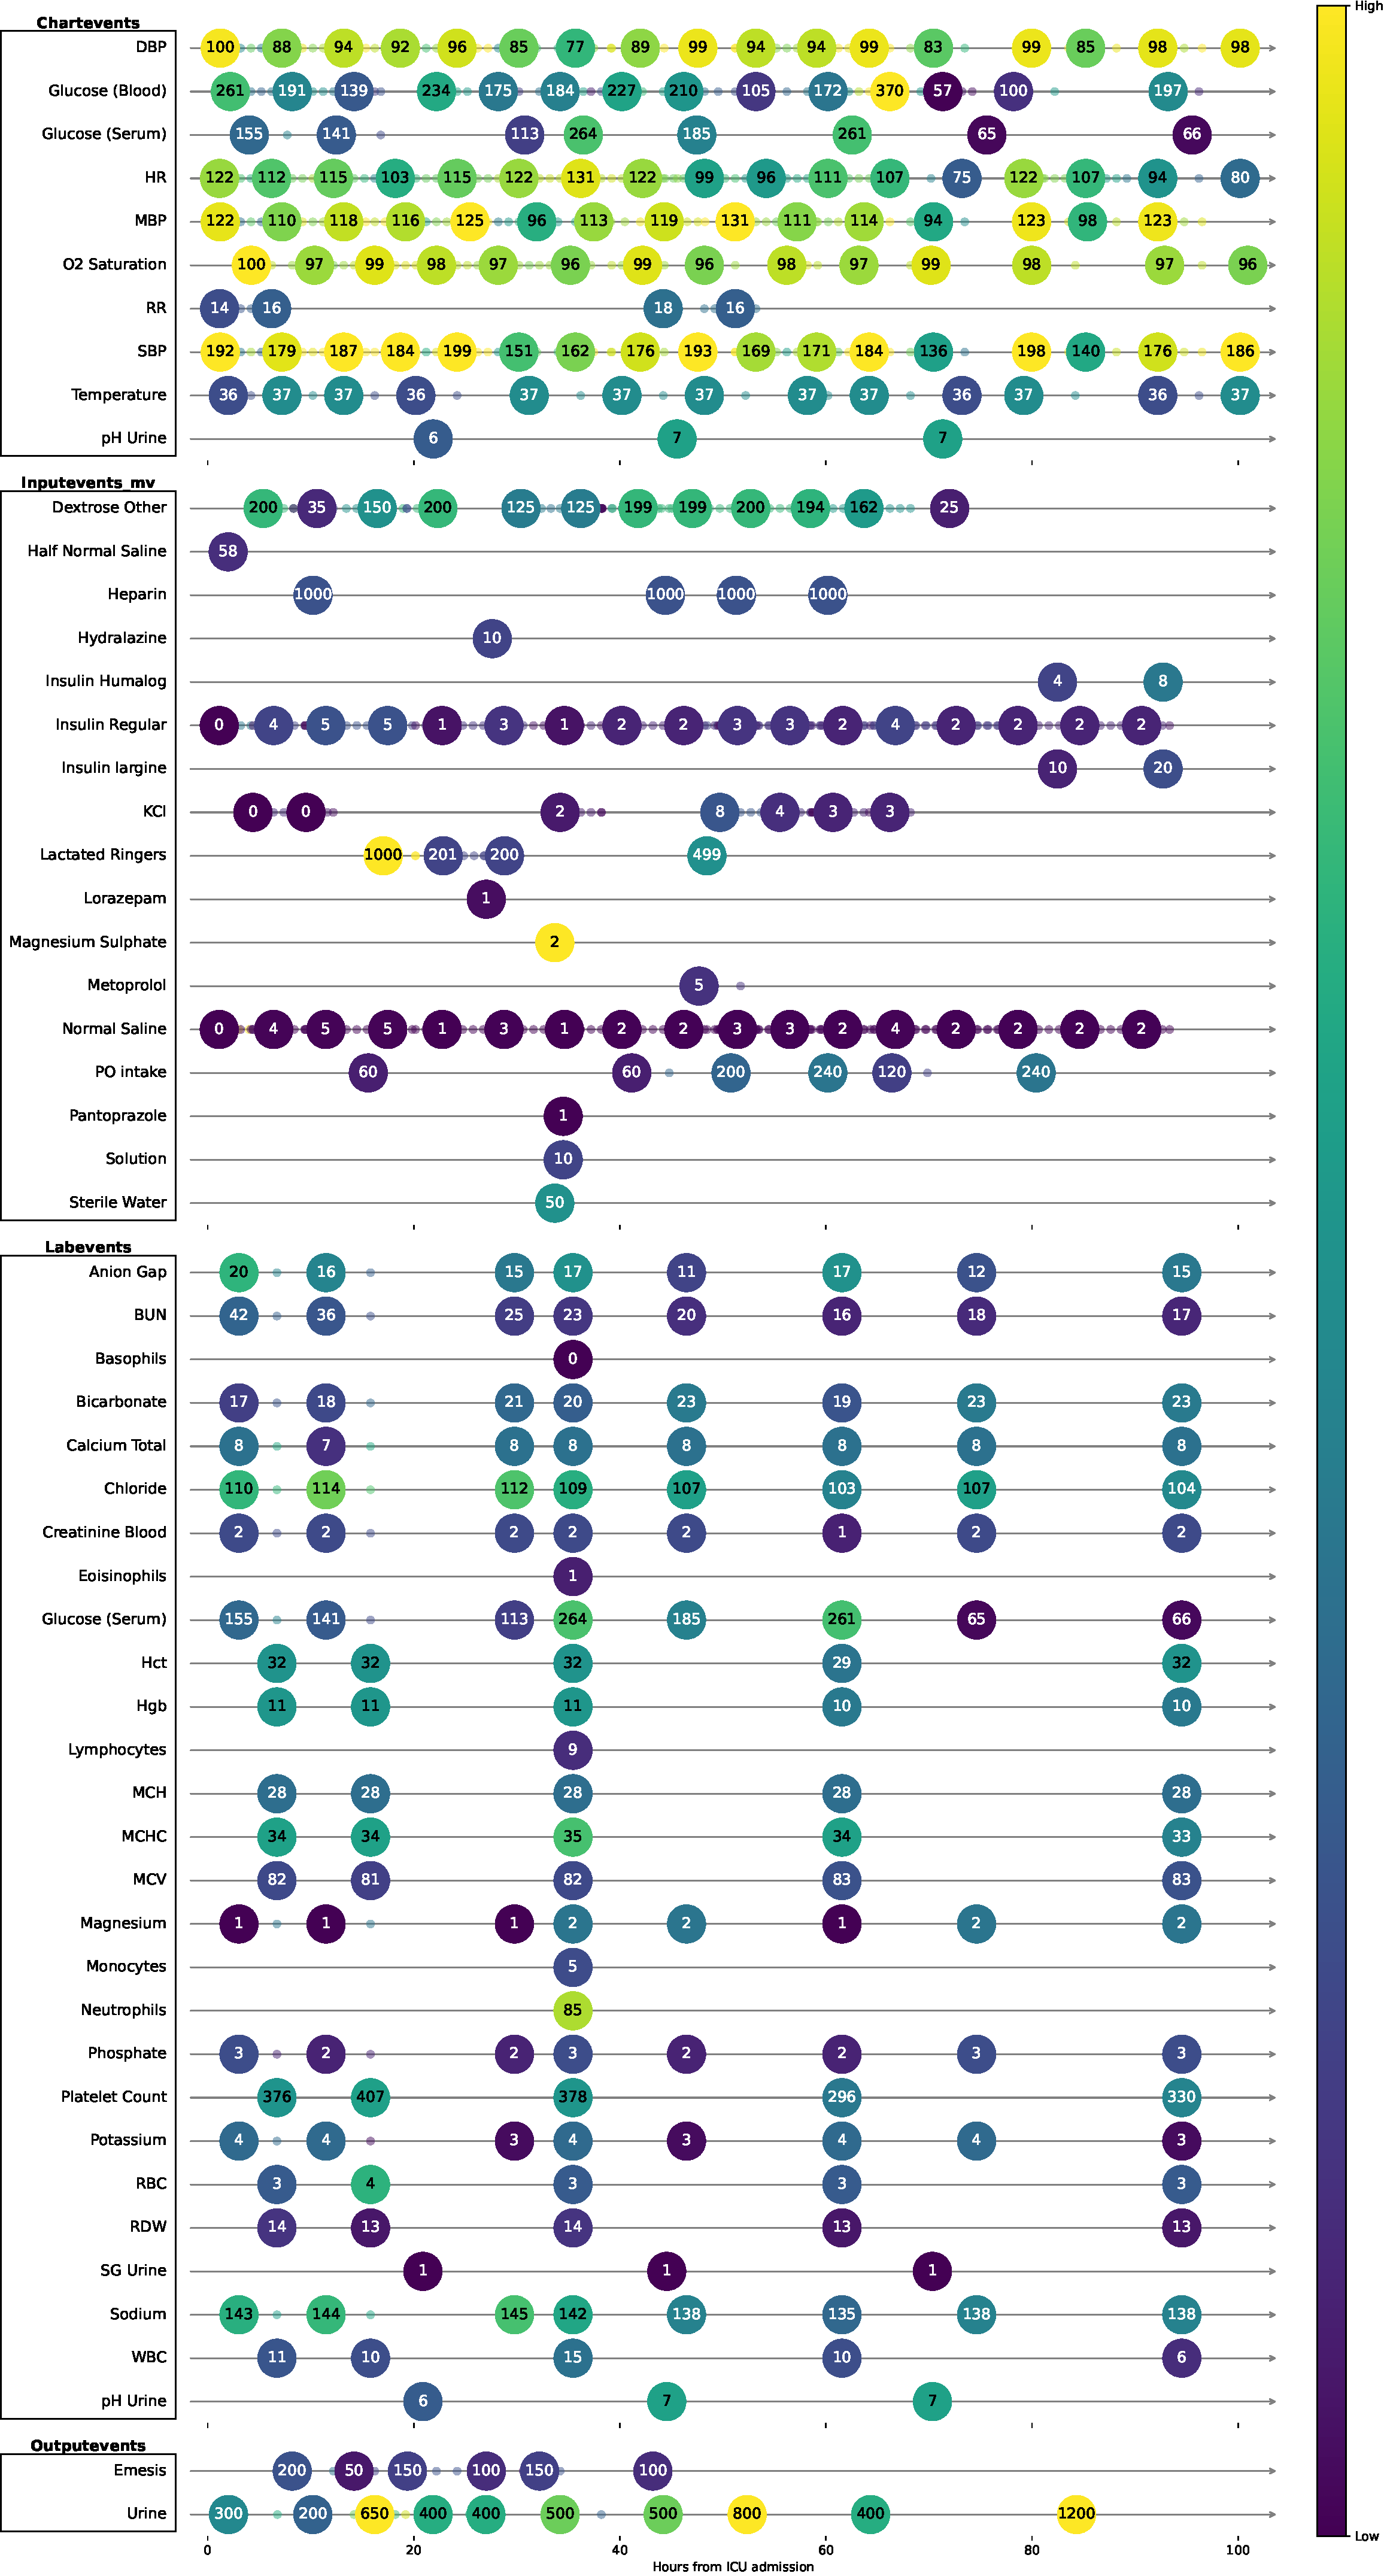
\includegraphics[height=0.95\textheight, width=\textwidth,keepaspectratio]{./figures/journey_275225}
    \caption{Visualization of a patient's journey with diverse measurements set. }
    \label{fig:journey_275225}
\end{figure}


\end{appendices}

\end{document}
